\documentclass[notitlepage, twoside, openright,12pt]{book}

%%%%%%%%%%%%%%%%%%%%%%%%%%%%%%%%%%%
%%%%  Pacchetti         
%%%%%%%%%%%%%%%%%%%%%%%%%%%%%%%%%%%
%%%%% Pagine bianche
\usepackage{afterpage}
\newcommand\blankpage{
    \null
    \thispagestyle{empty}%
    %\addtocounter{page}{-1}%
    \newpage}

%%%%% Testo di prova
\usepackage{lipsum}  


%%%%% TOC 
\usepackage[titles]{tocloft}

%%%% CITAZIONI
\usepackage{epigraph}
\setlength{\epigraphwidth}{0.64\textwidth}

\usepackage[absolute,overlay]{textpos}

%%%% VERBATIM INLINE
\usepackage{fancyvrb}



%%%% Sezioni di codice
\usepackage{listings}
\renewcommand\lstlistingname{Code}
\renewcommand\lstlistlistingname{List of codes}





%%%% Lingua e tastiera
\usepackage[english]{babel}
\usepackage[utf8]{inputenc}

\usepackage[a4paper,top=3cm, bottom=3cm, left=3.5cm, right=3.5cm]{geometry}

%%%% Matematica
\usepackage{amsmath}
\usepackage{amssymb}
\usepackage{amsthm}
\usepackage{xfrac}  %per le frazioni oblique
\usepackage{bm}  %bold in math mdoe


%%%% Tabelle e diagrammi
\usepackage{array}
\newcolumntype{L}{>{$}l<{$}}
\newcolumntype{S}[1]{>{\raggedright\arraybackslash}m{#1}}
\newcolumntype{M}[1]{>{\centering\arraybackslash}m{#1}}
\newcolumntype{D}[1]{>{\raggedleft\arraybackslash}m{#1}}
\usepackage[table]{xcolor}
\usepackage{xcolor}
\usepackage{./Settings/nicematrix}
\usepackage[all]{xy}

\usepackage{multirow} %Merge cell

%%%% Bibliografia
\usepackage{csquotes}
\usepackage[style=alphabetic, maxnames=5,minnames=4, backend=biber]{biblatex}
\addbibresource{biblio.bib}


%%%% Immagini
\usepackage{graphicx}
\usepackage{caption}
\usepackage{subcaption}


%%%% Oggetti flottanti
\usepackage{float}


%%%% Personalizzazione capitoli e intestazioni
\usepackage{titlesec}
\usepackage{fancyhdr}
\setlength\headheight{16pt}
\fancyhf{}


%%%% Togliere le intestazioni dalle pagine vuote
\usepackage{emptypage}


%%%% Pdf/a per consegna
\usepackage[a-1b]{pdfx}


%%%% Links
\usepackage[pdfa]{hyperref}


%%%% LANDSCAPE
\usepackage{lscape}



%%%%%%%%%%%%%%%%%%%%%%%%%%%%
%%%% Ambienti matematici %%%%
%%%%%%%%%%%%%%%%%%%%%%%%%%%%

\theoremstyle{plain}
\newtheorem{teo}{Theorem}[section]
\newtheorem*{teo*}{Theorem}
\newtheorem{lemma}[teo]{Lemma}
\newtheorem{cor}[teo]{Corollary}
\newtheorem{prop}[teo]{Proposition}
\theoremstyle{definition}
\newtheorem{defi}[teo]{Definition}
\newtheorem{nota}[teo]{Notation}
\theoremstyle{remark}
\newtheorem{oss}[teo]{Remark}
\newtheorem{ese}[teo]{Example}


%%%% COMANDI MATEMATICI NUOVI
\newcommand{\indep}{\perp \!\!\! \perp}

%%%%%%%%%%%%%%%%%%%%%%%%%%%%%%%
%% STILE CAPITOLI E SECTION     
%%%%%%%%%%%%%%%%%%%%%%%%%%%%%%%

%%%%%% Comandi personalizzati
\renewcommand{\thechapter}{\Roman{chapter}}

\renewcommand\theequation{\arabic{equation}}



%%%%%%% STILE 0 = (213280)mpd(5)
%\definecolor{gray75}{gray}{0.75}
%\titleformat{\chapter}[block]
%{\Huge\bfseries}
%{\thechapter\hspace{10pt}\textcolor{gray75}{\vline width 4pt}\hspace{10pt}}
%{0pt}
%{\Huge\bfseries}

%\titleformat{\section}
 %  {\normalfont\Large\bfseries}{\thesection}{1em}{}
%%%%%%%%%%%%%%%%%%%%

%%%%%%% STILE (STEFANO COSTA).1
%\usepackage{lmodern}
%\usepackage[explicit]{titlesec}
%\usepackage{microtype}
%\usepackage{tikz}

%\titleformat{\chapter}[hang]%
%{\bfseries}{%
%\begin{minipage}[t]{0.3\linewidth}  
%\vspace{0pt}% do not remove
%\begin{tikzpicture}
%\node[
%outer sep=0pt,
%text width=1.7cm,
%minimum height=2cm,
%fill=black,
%font=\color{white}\fontsize{60}{60}\selectfont,
%align=center
%] (num) {\thechapter};
%\node[
%outer sep=0pt,
%inner sep=0pt,
%anchor=south,
%font=\color{black}\Large\normalfont
%] at ([yshift=5pt]num.north) %{\textls[150]{\textsc{\chaptertitlename}}};
%\end{tikzpicture}  
%\end{minipage}}
%{0pt}%
%{\begin{minipage}[t]{.7\linewidth}%
%    \vspace{6pt} % do not remove
%    \rule{\linewidth}{2pt}\\\vskip -1.75\baselineskip%
%    \rule{\linewidth}{.7pt}\vskip 10pt
%    {\LARGE\raggedright\textsf{#1}}
%\end{minipage}}
%%%%%%%%%%%%%



%%%%%%% STILE (STEFANO COSTA).2
%\usepackage{lmodern}
%\usepackage[explicit]{titlesec}
%\usepackage{microtype}
%\usepackage{tikz}

%\titleformat{\chapter}[hang]%
%{\bfseries}{%
%\begin{minipage}[t]{0.3\linewidth}  
%\vspace{0pt}% do not remove
%\begin{tikzpicture}
%\node[
%outer sep=0pt,
%text width=1cm,
%minimum height=2.5cm,
%fill=black,
%font=\color{white}\fontsize{20}{20}\selectfont,
%align=center
%] (num) {\thechapter};
%\node[
%outer sep=0pt,
%inner sep=0pt,
%anchor=south,
%font=\color{black}\Large\normalfont
%] at ([yshift=5pt]num.north) %{\textls[5]{\textsc{\chaptertitlename}}};
%\end{tikzpicture}  
%\end{minipage}}
%{-20pt}%
%{\begin{minipage}[t]{.7\linewidth}%
%    \vspace{6pt} % do not remove
%    \rule{\linewidth}{2pt}\\\vskip -1.75\baselineskip%
%    \rule{\linewidth}{.7pt}\vskip 10pt
%    {\LARGE\raggedright\textsf{#1}}
%\end{minipage}}
%%%%%%%%%%%%


%%%%%%%% STILE (STEFANO COSTA).3
\usepackage{xhfill}

\titleformat{\chapter}[display]
{\filcenter}{\mbox{}\xrfill[0.4ex]{3pt}[black]\enspace\textsc{\Large\thechapter}\enspace\xrfill[0.4ex]{3pt}[black]\mbox{}}{0.3ex} {{\color{black}\titlerule[1pt]}\vskip3ex\LARGE\textsf\huge\bfseries}[\medskip{\color{black}\titlerule[1pt]}]



%%%%%%% STILE 1
%\titleformat{\chapter}[frame]
%{\normalfont\huge}
%{\chaptertitlename\ \thechapter}
%{20pt}
%{\bfseries\LARGE}

%%%%%%% STILE 2
%\titleformat{\chapter}[display]
%{\normalfont\Large\filcenter\sffamily}
%{\LARGE\MakeUppercase{\chaptertitlename} \thechapter}
%{1pc}
%{\titlerule \vspace{1pc} \LARGE\normalfont\raggedright}[\vspace{1ex}\titlerule]

%%%%%%% STILE 3
%\titleformat{\chapter}[frame]
%{\normalfont}
%{\filleft \enspace Chapter  \thechapter \enspace}
%{8pt}
%{\filcenter\Large\sffamily}
%%%%%%%%%%%%%%%%%%%

%%%%%%% STILE 4
%\titleformat{\chapter}[display]
%  {\bfseries\Large}
%  {\filright\MakeUppercase{\chaptertitlename} \Huge\thechapter}
%  {1ex}
%  {\titlerule\vspace{1ex}\filleft}
%  [\vspace{1ex}\titlerule]










%%%%%%%%%%%%%%%%%%%%%%%%%%%%%%%
%% STILE CODICE    
%%%%%%%%%%%%%%%%%%%%%%%%%%%%%%%
\definecolor{codegreen}{rgb}{0,0.6,0}
\definecolor{codered}{HTML}{cc0029}
\definecolor{background}{RGB}{230, 243, 252}



\lstdefinestyle{mystyle}{
    language=Python,
    backgroundcolor=\color{background}, 
    keywordstyle=\bfseries\color{blue},
    commentstyle=\itshape\color{codegreen},
    numberstyle=\tiny\color{black},
    stringstyle=\color{codered},
    basicstyle=\linespread{0.85}\ttfamily\footnotesize,
    firstnumber=0,  %%numeri partono da 0
    stepnumber=5,   %%numero ogni 5 righe
    frame=single,
    rulecolor=\color{black},  %colore frame
    breakatwhitespace=true,         
    breaklines=true,                 
    captionpos=t,      
    abovecaptionskip=10pt,
    belowcaptionskip=10pt,
    keepspaces=true,                 
    numbers=left,                    
    numbersep=10pt,                  
    showspaces=false,                
    showstringspaces=false,
    showtabs=false,                  
    tabsize=2,
    deletekeywords=[2]{map},
}

\lstset{style=mystyle}




%%%% P di probabilità
\newcommand{\probP}{\text{I\kern-0.18em P}}



%%%%%%%%%%%%%%%%%%%%%%%%%%%%%%%%%%
%%      INIZIO DOCUMENTO        %%
\begin{document}
%%%%%%%%%%%%%%%%%%%%%%%%%%%%%%%%%%





%%%%%%%%%%%%%%%%%%%%%%%%%%%%%%%
%% Frontmatter       
%%%%%%%%%%%%%%%%%%%%%%%%%%%%%%%
\frontmatter



%%%%%FRONTESPIZIO
\thispagestyle{empty}  


%%%% LOGO %%%%%
\begin{figure}[H]
\centering

\includegraphics{images/dmtesi.png}
\end{figure}

%%%% Corso di Laurea %%%%%%
\setlength{\parskip}{-12pt} % Modificare per spaziare diversamente le righe
%\noindent\rule{\textwidth}{1pt}
\begin{center}
\vspace{0.5cm}
\Large Bachelor's Degree in Mathematics
\end{center}
%\noindent\rule{\textwidth}{1pt}
%%%%%%%%%%%%%%%

\vspace{5 cm} % Aggiustare a piacere


%%%% Titolo %%%%%%
\begin{center}
{\fontsize{20}{30} \selectfont GAUSSIAN PROCESSES AND SUPERVISED LEARNING: APPLICATION TO THE WINDKESSEL MODEL \par} %}
\end{center}
%%%%%%%%%%%%%%%


\vspace{6 cm} % Aggiustare a piacere


\begin{large}
\begin{tabular}{m{7cm}l}
Candidate: & Supervisor:\\
Stefano Costa & Prof. Lucas Omar Müller
\end{tabular}
\end{large}


\vfill % Manda il resto a fondo pagina

%%%% Anno accademico %%%%%
\setlength{\parskip}{-18pt} % Modificare per spaziare diversamente le righe
%\noindent\rule{\textwidth}{1pt}
\begin{center}
{Academic Year 2021-22}
\end{center}
%\noindent\rule{\textwidth}{1pt}
\setlength{\parskip}{0pt} % Rimettere il parskip di default % frontespizio senza intestazioni



\chapter*{Ringraziamenti}
\thispagestyle{empty}

Ringrazio il mio relatore, il professor Lucas Omar Müller, per la sua pazienza, la sua guida e il suo sostegno. Ho tratto grande beneficio dalle sue conoscenze e dai suoi consigli, senza i quali questa tesi non sarebbe stata possibile.\\

Un doveroso ringraziamento va anche al dottor Christian Contarino, che non solo è stato fondamentale per la scelta e lo sviluppo dell'argomento, ma mi ha dato un costante sostegno morale.
\clearpage


%%%TOC
\pagestyle{plain} % indice col solo numero di pagina
\setcounter{tocdepth}{1}


\setlength\cftsecnumwidth{30pt}  %distanza della sezione dopo il numero
\setlength\cftchapnumwidth{30pt} %distanza del chapter dopo il numero


\tableofcontents
\addtocontents{toc}{~\hfill\textbf{Pag.}\par} %aggiunge Pag.



\newpage






%% LISTA CODICI

%Distanza dal numero a sinistra
\makeatletter
\def\l@lstlisting#1#2{\@dottedtocline{1}{1.5em}{3.5em}{#1}{#2}}
\makeatother

\setcounter{tocdepth}{2}
\lstlistoflistings
\addcontentsline{toc}{chapter}{List of codes}


\cftsetindents{figure}{1.5em}{3.5em}  %distanza dal numero a sinistra

\listoffigures
\addcontentsline{toc}{chapter}{List of figures}


\listoftables
\addcontentsline{toc}{chapter}{List of tables}











%%%%%%%%%%%%%%%%%%%%%%%%%%%%%%%
%% Intestazione per l'introduzione
%%%%%%%%%%%%%%%%%%%%%%%%%%%%%%%

%\pagestyle{fancy}
%\fancyhf{}

%\fancyfoot[C]{\thepage}
%\renewcommand{\headrulewidth}{0pt}
%\renewcommand{\footrulewidth}{0pt}










%% MAINMATTER
\mainmatter


%%%%%%%%%%%%%%%%%%%%%%%%%%%%%%%
%%%%% Intestazione per il corpo principale del documento
%%%%%%%%%%%%%%%%%%%%%%%%%%%%%%%
\pagestyle{fancy}

\fancyhead[LOH]{\nouppercase\rightmark}
\fancyhead[ROH]{\textbf{\thepage}}

\fancyhead[LEH]{\textbf{\thepage}}
\fancyhead[REH]{\nouppercase \leftmark }
\renewcommand{\headrulewidth}{0pt}
\renewcommand{\footrulewidth}{0pt}

%Cambia in alto a destra il capitolo:
%   (nome capitolo)      |  Capi. (#capitolo)
\renewcommand{\chaptermark}[1]{\markboth{#1 \qquad $\vert$ \quad  Ch. \thechapter\quad}{}}

%Cambia in alto a sinistra la sezione:
% sezione: (num sezione) | (nome sezione
\renewcommand{\sectionmark}[1]{\markright{\quad Sect. \thesection \quad $\vert$ \qquad ~#1}}




%%%%%% 
%%    Rimuove il numero di pagina dei capitoli
\makeatletter
\let\oldchapter\chapter  %salvo il comando chapter per richiamarlo dopo in modo che nella bibliografia compaia il numero di pagina
\renewcommand\chapter{\if@openright\cleardoublepage\else\clearpage\fi
                    \thispagestyle{empty}%
                    \global\@topnum\z@
                    \@afterindentfalse
                    \secdef\@chapter\@schapter}
\makeatother
%%%%%%%





%%%%%%%%%%%%%%%%%%%%%%%%%%%%%%
%%%%%%%%%%%% CAPITOLI
%%%%%%%%%%%%%%%%%%%%%%%%%%%%%%

\chapter{Introduction}
In the introductory chapter, the topics covered in the paper are motivated and introduced, and the main objective is explained: the application to the Windkessel model of supervised learning with Gaussian processes. The organization of the paper in terms of chapters, sources, images and code is then shown.

\begin{textblock*}{0.64\textwidth}(3.5cm+0.36\textwidth,18.5cm)
\epigraph{\textbf{Breve dialogo con punto di circonferenza}\\
- Per il Centro, mi scusi, qual è la via?\\
- Oh non si affanni, qui è tutto periferia.}{Marco Furgeri}
\end{textblock*}

\newpage




\section{Topics covered and motivation}
\subsection{Gaussian processes}
One of the main topics covered in the paper is supervised learning, that is, the problem of learning relationships between inputs and outputs from an example dataset and then making predictions about new inputs that the machine has never seen. It is therefore clear that the problem at hand is inductive: one must define (finite) training data $D$ and a function $f$ that makes predictions for all possible input values.\\
One approach to the problem is to define a class of functions from which to draw (e.g., linear functions), but this presents a problem: the choice of class. Indeed, this choice is very delicate since it can lead, for example, to a model based on functions that fail to accurately model the target function; in that case, predictions will be inaccurate. Furthermore, increasing the size of the class of functions (e.g., by increasing their parameters in a parametric regression context) does not necessarily improve the predictions, since there is a risk of \textit{overfitting}, in which a good fit to the training data is obtained but a poor result in predictions on new data.\\
A second approach is to assign a probability to each possible function, where higher probabilities are assigned to functions that are considered more likely, for example, because they are smoother (in terms of continuity). This approach is not without problems: there are an infinite number of possible functions and one is interested in evaluating this set in finite time. Gaussian processes elegantly solve this problem by generalizing the Gaussian probability distribution. While a probability distribution describes random variables that are scalars or vectors, this type of stochastic process governs the properties of functions. Intuitively, one can think of a function as a very long (infinite) vector in which each component is the value of the function $f(x)$ for some $x$. Throughout this work, it is explained how, although a simple idea, this solves the above problem. In fact: inference in Gaussian processes is able to draw conclusions from the properties of the function on a finite number of points, thus ignoring infinitely many. To do so, the function in question is considered as a vector with $f(x_i)$ components for $i=1,...,N$ which, because of the properties of Gaussian processes, is manipulated using multivariate Gaussian random variable theory, i.e., a relatively simple theory. This is extremely powerful because it is perfectly adaptable computationally. While not a well-known approach, in reality many models commonly used in machine learning and statistics are actually special cases or limited types of Gaussian processes. 

\newpage

\subsection{Windkessel model}

Haemodynamic models based on simplified representations of the components of the cardiovascular system can contribute strongly to the study and understanding of circulatory physiology and pathology. 
These models can be derived from the Navier-Stokes equations by exploiting specific features of blood flow, such as the cylindrical morphology of vessels, and can offer a great level of detail and a potentially accurate description of relevant quantities, but their numerical discretization is very complex and requires high computational resources.

The representation and analysis of the cardiovascular system (within what are known as zero-dimensional models) began with the modeling of arterial flow using the Windkessel model. In particular, it is the two-element Windkessel model, first proposed by Stephen Hales in 1733 and later mathematically formulated by Otto Frank in 1899, that is among the simplest and best known (zerodimensional) models. It consists of a capacitor $C$, which describes the elasticity properties of large arteries, and a resistor $R$ (divided into two resistors $R1$ and $R2$), which describes the dissipative nature of small peripheral vessels, including arterioles and capillaries. The modeling was then expanded to cover the modeling of other cardiovascular components, such as the heart, heart valves, and veins to simulate the overall hemodynamics of the entire circulatory system.

%È importante sottolineare che la meccanica del sistema cardiovascolare può presentare forti non linearità. Tra queste non linearità, le equazioni costitutive dipendenti dalla pressione e le proprietà dei vasi rappresentano un esempio di grande interesse. Ad esempio nell'elaborato, nella descrizione del modello Windkessel, i valori delle componenti $C$ e $R$ ($=R_1+R_2$) sono considerati costanti mentre, poiché rappresentano parametri fisici reali, sono soggetti a non linearità. Quando il diametro del vaso cambia in base alle variazioni di pressione, la sua capacitanza cambia, così come la sua resistenza al flusso. Questi effetti sono generalmente inclusi in modelli più complessi (uno dimensionali).

%Una comprensione approfondita della propagazione delle onde di pressione e di flusso nel sistema cardiovascolare e dell'impatto delle malattie e delle variazioni anatomiche su questi modelli può fornire informazioni preziose per la diagnosi clinica e il trattamento di patologie.
However, modeling blood flow in highly complex networks can involve computationally expensive simulations. 
%L'elevato costo computazionale e il tempo di esecuzione aumentano significativamente quando si devono simulare lunghi intervalli temporali, arrivando a richiedere diversi minuti per ogni ciclo cardiaco. 
The situation worsens when, for example, one wants to integrate different mechanisms in the cerebral microcirculation, such as cerebral perfusion or solute exchange between the blood and various tissue beds.

Several papers can be found in the literature concerning models for the simulation of arterial blood flow that address the issues of runtime and topological complexity optimization. Of interest in this work, however, is to exploit the capabilities of the Windkessel model (with easy generalization to other hemodynamic models) without having to solve the differential equation that describes it. In the Windkessel model, there is only one differential equation, so the computational cost and time required to get an approximation of the solution are very low. However, exploiting supervised learning with Gaussian processes yields the same results as in the Windkessel model (within a certain region of uncertainty) without solving the differential equation, thus decreasing the running time. In this simple case, there is no noticeable improvement, but thinking about very complex models with many differential equations, which generally require long run times and even hosting on supercomputers, acceptable run times in clinical settings can be achieved with this approach.

\newpage

\subsection{Justification of the topic}
Computational Life is a company founded in 2018 by Dr. Christian Contarino (Ph.D. at the University of Trento in 2018) focusing on biomedical applications of mathematics. Most recently, he is working on Altegos™, a patient-specific predictive decision support software that leverages the predictive technology of supervised learning in Gaussian processes. 

As anticipated, complex hemodynamic models (e.g., comprehensive models that model all components of the circulation) take a long time to run, which can be up to several hours. In a research setting this is not problematic, but in a clinical setting where one interfaces with patients who need urgent care this wait is incompatible. As anticipated then, Gaussian processes solve the run-time problem, allowing for support of a hemodynamic model that would potentially take hours to run.

In addition, Gaussian processes (and specifically the library used in the paper under \ref{Capitolo: risultati training}) allow for the study of the \textit{global sensitivity analysis} of parameters, making it possible to understand which among them actually have influence in a given output and which can be discarded from the study. This makes it possible to lighten machine learning by providing the statistical model with fewer parameters, sometimes many fewer, speeding up the process and improving accuracy (similar to what was concluded about $P_d$ in \ref{sensitività}).

These features were implemented in the research enterprise context by the research team coordinated by Dr. Contarino to create the Altegos™ product. In addition, the choice of Gaussian processes is justified by the fact that they have already shown excellent results in domains similar to the one studied in the paper (e.g., in \cite{doi:10.1098/rsta.2019.0334} and in \cite{Yuhn2022.03.10.483573}) and allow for an indication of prediction accuracy in the form of mean and standard deviation. This makes them a preferable choice to other machine learning approaches.


It is therefore evident that this technology and its application are novelties in the world of research and that its study constitutes an important addition to the academic background of a bachelor's degree student. This work, therefore, aims to study this technology applied in a simplified context, namely that of the Windkessel model, so that it can be easily generalized to more real-world and complex contexts such as those addressed in the master's degree. 

\newpage
\section{Organization of the work}
\subsection{Sources}
Each chapter is given an introductory page in which the content is anticipated and the sources used in writing it are cited.
The main source used for the part of Gaussian processes is \cite{rasmussen_gaussian_2006}; for the part related to hemodynamics and the Windkessel model important source of information was Professor Lucas Omar Müller author of \cite{ghitti_toro_müller_2022} and of the jupyter notebook that provided practical results on the Windkessel model (later extensively modified); the python library "GPErks," which can be found on GitHub, was used in the chapter "Methodology and Training Results".

\subsection{Images}
Most of the images were generated by the author of the work; of these the python code is often given in the appendix\footnote{Not of all the images are the codes for generating them given because in some cases it was too massive to include in the paper and sometimes not very useful: the codes for the GPErks library, for example, can be found on the GitHub page and there is no need to include them in the paper}. Of all images not generated by the author, the source can be found in the caption.

\subsection{Code}
The code written for generating the images and the results obtained is written in python. This choice was made because python allows many options in graph creation and because the GPErks library is written in python.

\newpage

\subsection{Structure of the work}
The first two chapters are intended to introduce the broad topic of Gaussian processes. The discussion will not devote itself to framing Gaussian processes in the broad context of stochastic processes but will limit itself to a focused study of its peculiarities useful for the purposes of supervised learning.\\

The chapter "Machine learning" introduces the concepts of Bayesian statistics underlying supervised learning focusing on the case of Gaussian processes. Some optimization methods including the one used to obtain the results shown in the last chapter are also introduced for informative purposes.\\

Next, the Windkessel model is introduced, showing only the differential equation (thus without explaining how to deduce it from the Navier-Stokes equation). Practical results on its use in predicting a patient's blood pressure from his flow are then illustrated. The chapter concludes with a study of the local sensitivity of MAP, DBP, SBP, and PP with respect to $C$ (compliance), $R_1$ (proximal resistance), $R_2$ (peripheral resistance), and $P_d$ (distal pressure), concluding that distal pressure has little influence on the variables, which is why it was excluded from the input parameters in supervised learning. \\

The last chapter shows the results obtained from training Gaussian processes following the GPErks library approach to study the $C$, $R_1$ and $R_2$ dependence of blood pressure.\\

The appendix contains most of the codes used for generating the images and results used in the paper.
\chapter{Gaussian distribution}
In this chapter, the basic properties of Gaussian distributions are given, with special attention in regard to the \textbf{multivariate Gaussian distribution}. As the name suggests, \textbf{Gaussian processes} are in fact based on these multivariate distributions, exploiting properties that will be shown throughout the chapter.\\
The sources used in writing the chapter are \cite{gut_intermediate_2009}, \cite{wilkinson_introduction_2020}, \cite{murphy_probabilistic_2022}.


\begin{textblock*}{0.64\textwidth}(3.5cm+0.36\textwidth,18.5cm)
\epigraph{At a purely formal level, one could call probability theory the study of measure spaces with total measure one, but that would be like calling number theory the study of strings of digits which terminate.}{Terence Tao}
\end{textblock*}

\newpage

%%%%%%%%%%%%%%%%%%%%%%%%%%%%%%%%%%%
%%%%%% GAUSSIANA UNIVARIATA
%%%%%%%%%%%%%%%%%%%%%%%%%%%%%%%%%%%


\section{Univariate Gaussian distribution}
\begin{defi}[Univariate Gaussian distribution]
    The \textbf{univariate Gaussian distribution} is a continuous probability distribution. \\
    Given $Y\sim \mathcal{N}(\mu, \sigma^2)$, its probability density function is expressed as:
    \[f_Y(y) = \frac{1}{\sqrt{2\pi \sigma^2}} \text{exp}\bigg\{-\frac{1}{2}\frac{(y-\mu)^2}{\sigma^2}\bigg\}.\]
\end{defi}


%%%%%%%%%%%%%%%%%%%%%%%%%%%%%%%%%%%
%%%%%% IMMAGINI GAUSSIANA
%%%%%%%%%%%%%%%%%%%%%%%%%%%%%%%%%%%
\begin{figure}[h]
\centering
\begin{subfigure}{.5\textwidth}
  \centering
  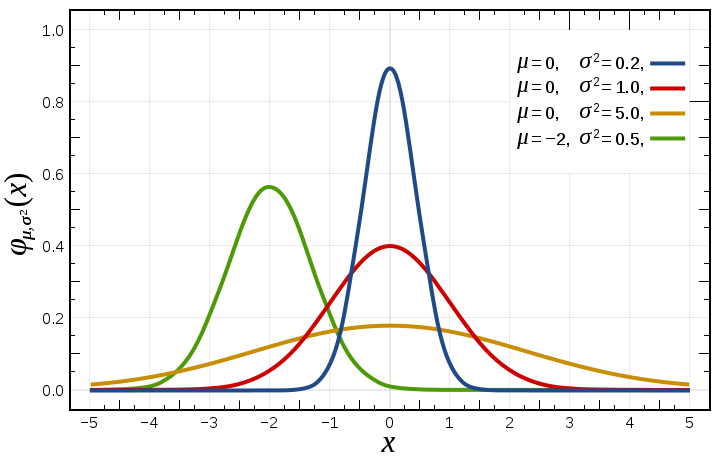
\includegraphics[width=\linewidth]{images/Gaussiane/PDFNormalDistribution.png}
  \caption{Probability density}
  \label{fig:sub1}
\end{subfigure}%
\begin{subfigure}{.5\textwidth}
  \centering
  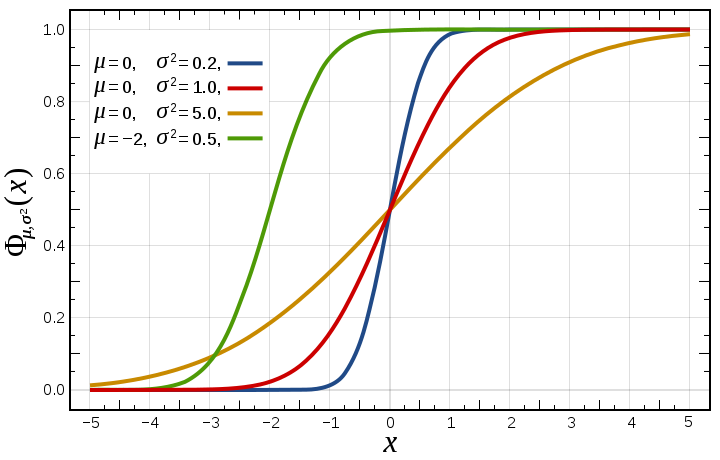
\includegraphics[width=\linewidth]{images/Gaussiane/CDFNormalDistribution.png}
  \caption{Distribution function}
  \label{fig:sub2}
\end{subfigure}
\caption{Distribution function and probability density of a standard normal distribution \cite{wikiNormalDistribution}.}
\label{fig:gaussian}
\end{figure}



\begin{oss} \label{normal decomposition}
Given $Z\sim \mathcal{N}(0,1)$ it follows:  $Y=\mu + \sigma Z\sim \mathcal{N}(\mu,\sigma^2)$.
\end{oss}

\begin{oss}
    Informally speaking, the Gaussian distribution is "convenient" mathematically because of its properties:
\begin{itemize}
    \item the normal distribution has two parameters that are easy to interpret: the mean and the variance;
    \item the normal distribution is closed under linear operations;
    \item the normal distribution is closed by marginalization and conditioning (see the proposition \ref{marginale-condizionata});
    \item at equal mean and variance, the normal distribution has maximum entropy;
    \item from \textbf{central limit theorem}, the normal distribution is the limit of a sum of random variables; 
    \item the normal distribution has a simple mathematical form that facilitates its implementation.
\end{itemize}
\end{oss}


\newpage


%%%%%%%%%%%%%%%%%%%%%%%%%%%%%%%%%%%
%%%%%% GAUSSIANA MULTIVARIATA
%%%%%%%%%%%%%%%%%%%%%%%%%%%%%%%%%%%
\section{Multivariate Gaussian distribution}


The multivariate Gaussian distribution is a generalization of the normal (univariate) distribution.



\begin{defi}[Multivariate Gaussian distribution] An $n$-dimensional $\mathbf{X}$-vector of random variables is said to be normal (\textbf{multivariate normal}) if and only if $\forall \mathbf{a} in \mathbb{R}^n$ the random variable $\mathbf{a}^\text{T}\mathbf{X}$ is a normal distribution.  
    The density\footnote{In the generalized case it is not possible to define the density of the multivariate Gaussian distribution. As will be shown later, in Gaussian processes the density is not as important as the covariance matrix and the mean vector.} of a \textbf{multivariate Gaussian distribution} is expressed as
\[f_{\mathbf{X}}(\mathbf{x})=\frac{1}{(2\pi)^{\sfrac{n}{2}}  \text{det}(\bm{\Sigma})^{\sfrac{1}{2}}} \text{ exp}\left[-\frac{1}{2}(\bm{x}-\bm{\mu})^\text{T}\bm{\Sigma}^{-1}(\bm{x}-\bm{\mu})\right]
\]\end{defi}
where $\bm{\mu}=\mathbb{E}[\bm{X}]\in \mathbb{R}^n$ is the  \textit{mean vector}, $\bm{\Sigma}=\text{Cov}[\bm{X}]$ is a $n\times n$ matrix called \textit{covariance matrix}, defined as:
\[\begin{split}
\text{Cov}[\bm{X}] &= \mathbb{E}\left[(\bm{X}-\mathbb{E}[\bm{X}])(\bm{X}-\mathbb{E}[\bm{X}])^\text{T} \right]\\
 & = \begin{pmatrix}
    \mathbb{V}[X_1] & \text{Cov}[X_1,X_2] & \dots & \text{Cov}[X_1,X_n]\\
    \text{Cov}[X_2,X_1] & \mathbb{V}[X_2] & \dots & \text{Cov}[X_2,X_n]\\
    \vdots & \vdots & \ddots & \vdots\\
    \text{Cov}[X_n,X_1] & \text{Cov}[X_n,X_2] & \dots & \mathbb{V}[X_n]
    \end{pmatrix}
\end{split}
\]
where:
\[ \text{Cov}[X_i,X_j]=\mathbb{E}[(X_i-\mathbb{E}[X_i])(X_j-\mathbb{E}[X_j])] = \mathbb{E}[X_iX_j]-\mathbb{E}[X_i]\mathbb{E}[X_j]  \]
\[ \mathbb{V}[X_i]=\text{Cov}[X_i, X_i]. \]


\begin{oss}\label{ossGaussianaMultivariata}
    The covariance matrix is symmetrical and semidefinite positive, i.e., $\forall \mathbf{a} \in \mathbb{R}^n$ one has $\mathbf{a}^\text{T} \mathbf{a}\geq 0$.
\end{oss}


%%%%%%%%%%%%%%%%%%%%%%%%%%%%%%%%%%%
%%%%%% COROLLARIO DEFINIZIONE
%%%%%%%%%%%%%%%%%%%%%%%%%%%%%%%%%%%
\begin{cor}
    Given $\mathbf{X}$ a multivariate normal vector, from the definition of multivariate Gaussian distribution follow immediately:
\begin{enumerate}
    \item each component of $\mathbf{X}$ is a Gaussian random variable;
    \item $\sum_{i=1}^{n} a_iX_i$ is a Gaussian random variable $\forall a_i\in \mathbb{R}$;
    \item If the components of $\mathbf{X}$ are independent Gaussian random variables, then $\mathbf{X}$ is a multivariate normal vector.
\end{enumerate}
\end{cor}

\begin{oss}
    The third point of the previous corollary does not hold if the components are not independent. For example: $X\sim \mathcal{N}(0,1)$, $Z\indep X$, $\mathbb{P}(Z=1)=\mathbb{P}(Z=-1)=\sfrac{1}{2}$. It is easily seen that $Y=ZX$ is not independent of $X$ and $\begin{pmatrix}
X\\
Y
\end{pmatrix}$ is not multivariate normal.
\end{oss}

\newpage


%%%%%%%%%%%%%%%%%%%%%%%%%%%%%%%%%%%
%%%%%% PROPOSIZIONE
%%%%%%%%%%%%%%%%%%%%%%%%%%%%%%%%%%%
Of critical importance is the next proposition. The proof is omitted because it consists of lengthy calculations that are outside the scope of the paper. For the proof, please refer to \cite{murphy_probabilistic_2022}.
\begin{prop}[Marginal and conditional distribution] \label{marginale-condizionata}
Let $\bm{Y}=\begin{pmatrix}\bm{y}_1 \\ \bm{y}_2\end{pmatrix}$ Gaussian multivariate vector where:
\[
\bm{\mu}=\begin{pmatrix}\bm{\mu}_1\\ \bm{\mu}_2\end{pmatrix}\quad
 \bm{\Sigma}=\begin{pmatrix}\bm{\Sigma}_{11}&\bm{\Sigma}_{12}\\ \bm{\Sigma}_{21}&\bm{\Sigma}_{22}\end{pmatrix}\quad \bm{\Lambda}=\bm{\Sigma}^{-1}=\begin{pmatrix}\bm{\Lambda}_{11}&\bm{\Lambda}_{12}\\\bm{\Lambda}_{21}&\bm{\Lambda}_{22}\end{pmatrix}
\]
Then the marginal distributions are:
\[
\bm{y}_1\sim \mathcal{N}(\bm{\mu}_1, \bm{\Sigma}_{11}) \qquad \bm{y}_2\sim \mathcal{N}(\bm{\mu}_2, \bm{\Sigma}_{22})
\]
While conditional distributions are:
\[
\bm{y}_1 | \bm{y}_2 \sim \mathcal{N}(\bm{\mu}_{1|2}, \bm{\Sigma}_{1|2}) \qquad
\def\arraystretch{1.4}
\begin{array}{l}
    \bm{\mu}_{1|2}        =\bm{\mu}_1+\bm{\Sigma}_{12}\bm{\Sigma}_{22}^{-1}(\bm{y}_2-\bm{\mu}_2)\\
    \bm{\Sigma}_{1|2}=\bm{\Sigma}_{11}-\bm{\Sigma}_{12}\bm{\Sigma}_{22}^{-1}\bm{\Sigma}_{21}=\bm{\Lambda}_{11}^{-1}
\end{array}
\]

\[
\bm{y}_2 | \bm{y}_1 \sim \mathcal{N}(\bm{\mu}_{2|1}, \bm{\Sigma}_{2|1})
\qquad
\def\arraystretch{1.4}
\begin{array}{l}
    \bm{\mu}_{2|1}        =\bm{\mu}_2+\bm{\Sigma}_{21}\bm{\Sigma}_{11}^{-1}(\bm{y}_1-\bm{\mu}_1)\\
    \bm{\Sigma}_{2|1}=\bm{\Sigma}_{22}-\bm{\Sigma}_{21}\bm{\Sigma}_{11}^{-1}\bm{\Sigma}_{12}=\bm{\Lambda}_{22}^{-1}
\end{array}
\]
\end{prop}

\newpage

%%%%%%%%%%%%%%%%%%%%%%%%%%%%%%%%%%%
%%%%%% CORRELAZIONE VETTORI
%%%%%%%%%%%%%%%%%%%%%%%%%%%%%%%%%%%
\section{Correlation for multivariate vectors} \label{sezioneCorrelazione}


\begin{defi}[Pearson's correlation index]
The \textbf{Pearson's correlation index} between two random variables is an index expressing a linearity relationship between them. It is expressed as:
\[ \rho_{XY}=\frac{\text{Cov}[X,Y]}{\sqrt{\mathbb{V}[X]\mathbb{V}[Y]}}.
\]
\end{defi}
\begin{oss}[Meaning of $\rho_{XY}$]
    Because of the Cauchy-Schwarz inequality it holds: $-1\leq \rho_{XY}=1$. There are three main cases: $\rho_{XY}=1$ indicates a perfect positive linear relationship; $\rho_{XY}=-1$ indicates a perfect negative linear relationship; $\rho_{XY}=0$ indicates no linear correlation. 
\end{oss}

The remainder of the chapter will focus on the analysis of bivariate Gaussian vectors and the correlation of their components and then generalize the visual approach to multiple dimensions.

%%%%%%%%%%%%%%%%%%%%%%%%%%%%%%%%%%%
%%%%%% CORRELAZIONE GAUSSIANI
%%%%%%%%%%%%%%%%%%%%%%%%%%%%%%%%%%%
Consider a two-dimensional Gaussian vector: \[\mathbf{Y}=\begin{pmatrix}Y_1\\Y_2\end{pmatrix} \qquad\text{con} \qquad \bm{\mu} = \begin{pmatrix}0\\0\end{pmatrix} \quad \mathbf{\Sigma}=\begin{pmatrix}1&0\\0&1\end{pmatrix}.
\]
Generating points from the distribution of $\mathbf{Y}$ (so each point consists of a two-dimensional vector) yields what is shown in figure \ref{correlazione1}.

%%%%%%%%%IMMAGINE
\begin{figure}[h]
    \centering
    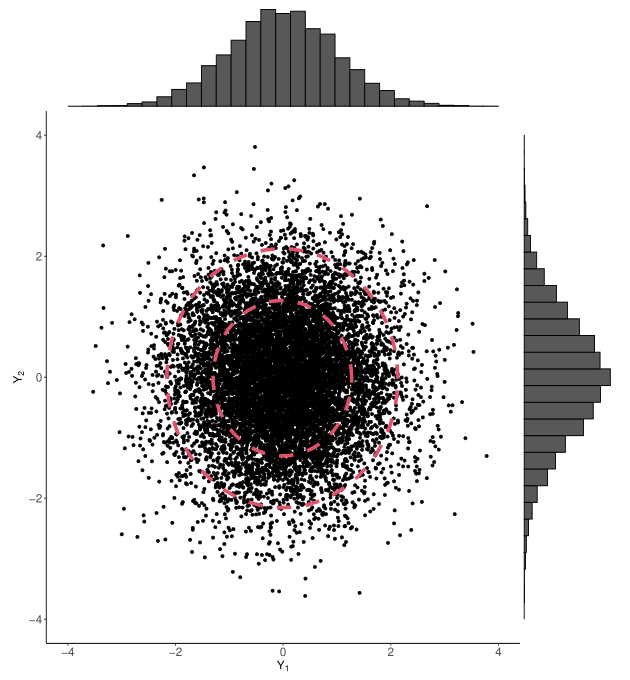
\includegraphics[width=0.65\textwidth]{images/Gaussiane/VettoreBivariatoIndipendenza.png}
    \caption{Point cloud generated by a bivariate Gaussian distribution with uncorrelated components \cite{wilkinson_introduction_2020}.}
    \label{correlazione1}
\end{figure}


\newpage
Note that the point cloud is centered in zero as a consequence of the choice of $\bm{\mu}$. It is easy to compute $\rho_{Y_1,Y_2}=0$ which guarantees the incorrelation of the components of the Gaussian vector. This result can be guessed from the shape of the cloud: given a point in the cloud, knowledge of its $Y_1$ coordinate gives no information about its $Y_2$ coordinate.\\
Now consider $\bm{\mu} = \begin{pmatrix}0\\0\end{pmatrix}$ e $\mathbf{\Sigma}=\begin{pmatrix}1&0.9\\0.9&1\end{pmatrix}$. Generating a cloud of points again yields what is shown in figure \ref{correlazione2}.\\

%%%%%%%%%IMMAGINE
\begin{figure}[h]
    \centering
    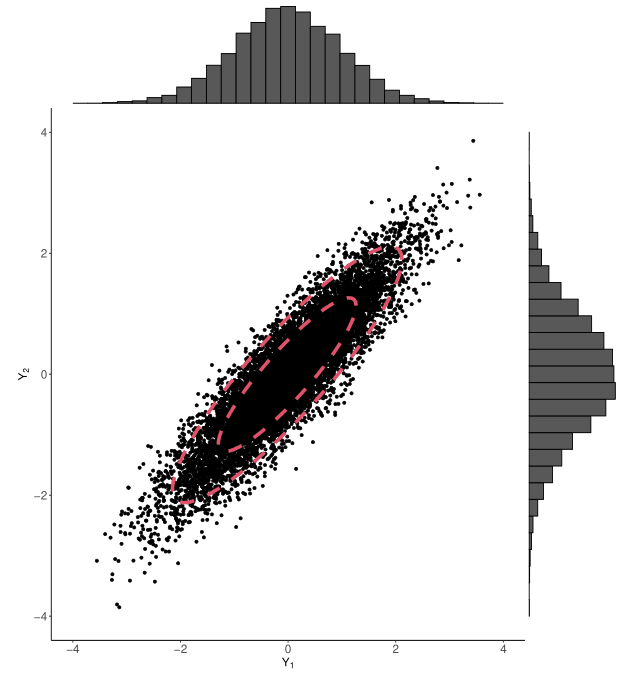
\includegraphics[width=0.7\textwidth]{images/Gaussiane/VettoreBivariatoIndipendenza2.png}
    \caption{Point cloud generated by a bivariate Gaussian distribution with correlated components \cite{wilkinson_introduction_2020}.}
    \label{correlazione2}
\end{figure}

From the shape of the cloud it is now possible to see the correlation between the components of the Gaussian vector. Given a point on the cloud, in fact, the first of the two components gives an approximate idea of the value of the second component (and vice versa): the cloud, to a certain approximation, thickens around a line passing through the origin.\\
The elliptical shape of the cloud is a consequence of the correlation index value: $\rho_{Y_1,Y_2}=0.9$, that is, there is a large linear correlation between the two components.\\

\newpage
Evidently, the elliptical shape becomes more pronounced as the value of the correlation index increases, as can be seen from the figure \ref{correlazione3}, in which $\mathbf{\Sigma}=\begin{pmatrix}1&0.99\\0.99&1\end{pmatrix}$ and thus $\rho_{Y_1,Y_2}=0.99$.

%%%%%%%%%%%IMMAGINE
\begin{figure}[h]
    \centering
    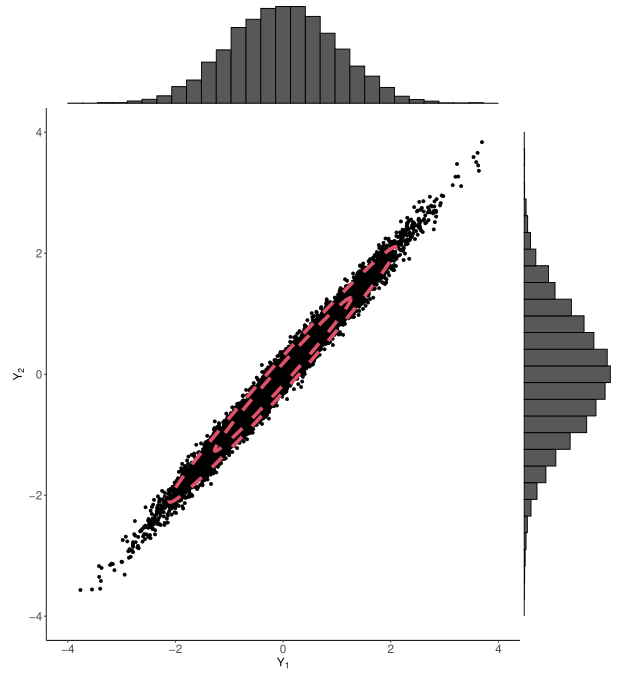
\includegraphics[width=0.7\textwidth]{images/Gaussiane/VettoreBivariatoIndipendenza3.png}
    \caption{Point cloud generated by a bivariate Gaussian distribution with strongly correlated components \cite{wilkinson_introduction_2020}.}
    \label{correlazione3}
\end{figure}



\newpage

In order to generalize to more than two dimensions the visual process of interpreting the correlation between the components of a multivariate Gaussian vector, it is necessary to adopt a different strategy: for each sample (i.e., for each vector) generated by the multivariate Gaussian distribution, the value of the components is plotted in a graph by connecting the respective values by a segment.\\
In figure \ref{correlazione4} the example in two dimensions with $\bm{\mu} = \begin{pmatrix}0\\0\end{pmatrix}$ and $\mathbf{\Sigma}=\begin{pmatrix}1&0.54\\0.54&0.3\end{pmatrix}$. The graph on the left shows the approach used so far; the graph on the right shows for each point on the left graph the value of the first component at index $1$ on the abscissae and the value of the second component at index $2$ on the abscissae.


%%%%%%%%%%%IMMAGINE
\begin{figure}[h]
    \centering
    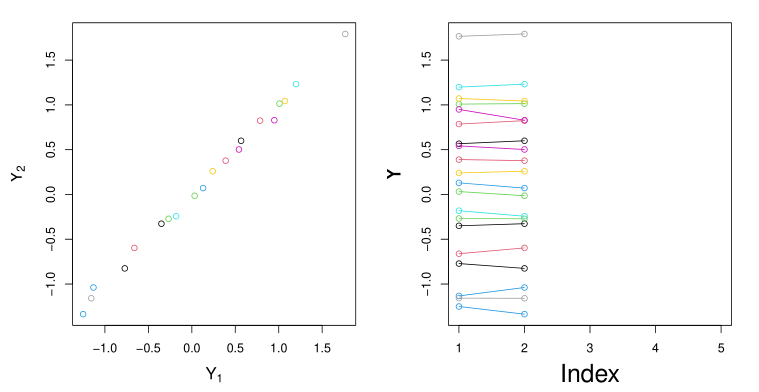
\includegraphics[width=\textwidth]{images/Gaussiane/CorrelazioneMultidimensionale.png}
    \caption{Two different visual approaches to correlation of components of multivariate Gaussian vectors: $n=2$ \cite{wilkinson_introduction_2020}.}
    \label{correlazione4}
\end{figure}


\newpage 

This approach allows generalization to dimensions $n>2$. Let it be now:
\[\bm{\mu}=\bm{0} \qquad\qquad \bm{\Sigma}=\begin{pmatrix}1&0.99&0.98&0.97&0.96\\0.99&1&0.99&0.98&0.97\\0.98&0.99&1&0.99&0.98\\0.97&0.98&0.99&1&0.99\\0.96&0.97&0.98&0.99&1 \end{pmatrix}
\]
Where the components are strongly correlated with each other. We obtain what is shown in the figure \ref{correlazione5}.

%%%%%%%%%%%IMMAGINE
\begin{figure}[h]
    \centering
    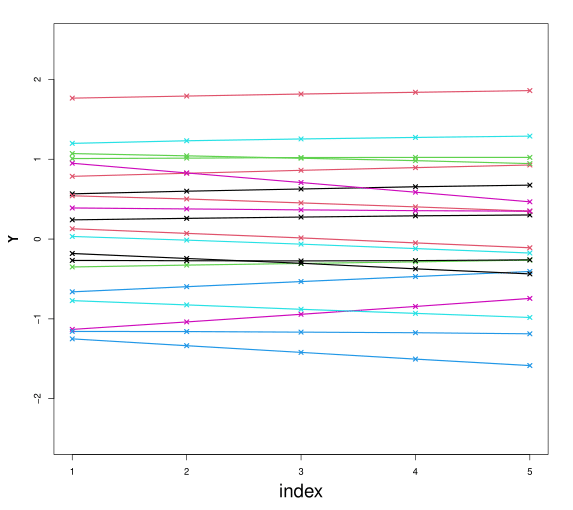
\includegraphics[width=0.7\textwidth]{images/Gaussiane/CorrelazioneMultidimensionale2.png}
    \caption{Visualization using segments of the correlation of components of multivariate Gaussian vectors: $n=5$ \cite{wilkinson_introduction_2020}.}
    \label{correlazione5}
\end{figure}

Being in dimension $n=5$, each sample generated by the Gaussian vector has five components, so when a sample is plotted in the graph it has five points at indices 1, 2, 3, 4, 5.
\newpage

In this case, the strong correlation between the components of the Gaussian vector is reflected in the segment joining the individual points of each sample, as shown in Figure \ref{SegmentCorrelation}.

%%%%%%%%%%%IMMAGINE
\begin{figure}[h]
    \centering
    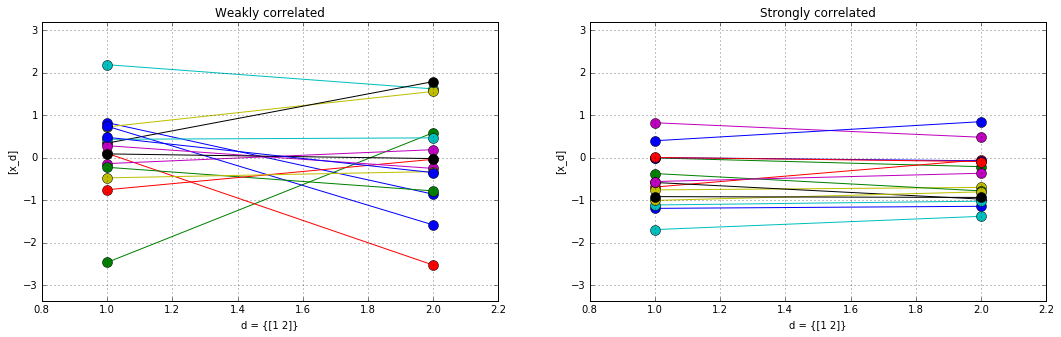
\includegraphics[width=1\textwidth]{images/Gaussiane/CorrelazioneUnidimensionale.png}
    \caption{Weak and strong correlation of components of multivariate Gaussian vectors visualized by segments \cite{damianou_gaussian_2016}.}
    \label{SegmentCorrelation}
\end{figure}

In the case $n=50$ (with null norm vector but omitting the covariance matrix, which continues to have one on the diagonal and values close to one in the other entries), we obtain what is in the figure \ref{correlazione6}.


%%%%%%%%%%%IMMAGINE
\begin{figure}[h]
    \centering
    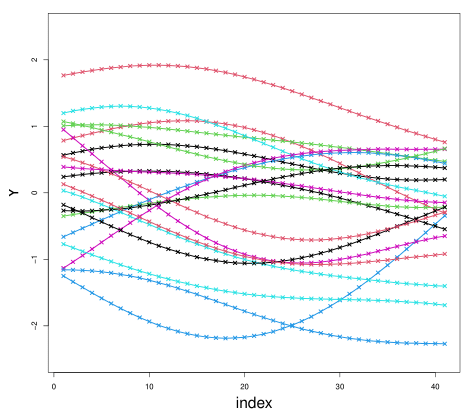
\includegraphics[width=0.7\textwidth]{images/Gaussiane/CorrelazioneMultidimensionale3.png}
    \caption{Visualization by segments of the correlation of components of multivariate Gaussian vectors: $n=50$ \cite{wilkinson_introduction_2020}.}
    \label{correlazione6}
\end{figure}

Notice then that as $n$ increases what obtained begins to resemble a function for each sample generated.\\
From this approach it is possible to interpret Gaussian processes either as functions or as infinite-dimensional multivariate Gaussian distributions ($n=\infty$) with a continuous index (introducing a \textit{mean function} and a \textit{covariance function}). This interpretation will be clarified in the next chapter.
\chapter{Gaussian processes}\label{gaussianProcessChapter}
This chapter introduces the \textbf{Gaussian processes}. Inevitably, the chapter will not be exhaustive of the subject, but its main features of interest for the purposes of the paper will be treated. For this reason, the discussion will not be devoted to framing Gaussian processes in the vast context of stochastic processes and will limit itself to a focused study of its peculiarities.\\
The python codes used in the chapter require executing the \ref{import} and \ref{import2} import codes of the libraries. Furthermore, the cubic mean is defined for all kernels as in the code \ref{cubedMean}. 
The code for the kernel images is inspired by that written by Peter Roelants in his blog on the page "\href{https://peterroelants.github.io/posts/gaussian-process-tutorial/#Gaussian-processes-(1/3)---From-scratch}{Gaussian processes - From scratch}". Important changes have been made to the code, in particular the kernels implemented by the scikit-learn library are used.
The code for data prediction, on the other hand, takes its inspiration from \href{https://docs.w3cub.com/about/}{W3cubDocs} on the page "\href{https://docs.w3cub.com/scikit_learn/auto_examples/gaussian_process/plot_gpr_noisy_targets}{Gaussian Processes regression: basic introductory example}". Again, important changes have been made in the code.
The code about the concentration of $CO_2$ is a modification of the code '\href{https://scikit-learn.org/stable/auto_examples/gaussian_process/plot_gpr_co2.html}{Gaussian process regression (GPR) on Mauna Loa CO2 data}' present in the scikit-learn documentation.\\
The sources used for the drafting of the chapter are: \cite{rasmussen_gaussian_2006}, \cite{murphy_probabilistic_2022}, \cite{rasmussen_gaussian_2004}, \cite{duvenaud_automatic_2014}, \cite{gortler_visual_2019}, \cite{murphy_machine_2012}.


\begin{textblock*}{0.64\textwidth}(3.5cm+0.36\textwidth,18.5cm)
\epigraph{In applying mathematics to subjects such as physics
or statistics we make tentative assumptions about the
real world which we know are false but which we believe
may be useful nonetheless. The physicist knows that
particles have mass and yet certain results, approximating
what really happens, may be derived from the assuhption that they do not. Equally, the statistician knows, for
example, that in nature there never was a normal distribution, there never was a straight line, yet with normal and
linear assumptions, known to be false, he can often derive
results which match, to a useful approximation, those
found in the real world.}{George E. P. Box}
\end{textblock*}

\newpage


%%%%%%%%%%%%%%%%%%%%%%%%%%%%%%
%%%%% DEFINIZIONE
%%%%%%%%%%%%%%%%%%%%%%%%%%%%%%
\section{Definition and motivation}


\begin{defi}[Gaussian process]
  A \textbf{Gaussian process} is a set of random variables such that every finite subset of it has a multivariate Gaussian distribution.
\end{defi}

It is evident from the definition that the theory of multivariate Gaussian distributions has considerable importance in the study of Gaussian processes.\\
Similar to the Gaussian distribution, which is completely determined by its mean vector and covariance matrix, Gaussian processes are completely determined by a \textit{mean function} (which determines its mean), denoted $m(x)$, and by a \textit{covariance function} (which determines the covariance), denoted $k(x,x')$. The role of the two functions will be discussed in more detail in the next section.\\
Despite this similarity, however, Gaussian distributions and Gaussian processes differ in one important characteristic: the former work with vectors, the latter with functions.

\vspace{0.5cm}

\begin{oss}[Motivation: nonlinear regression]
  The main application of Gaussian processes, and the main theme of this chapter, is \textbf{nonlinear regression}.\\
  While the linear regression model seeks, from observed data, a linear relationship between a dependent variable $Y$ and an independent variable $x$, taking into account a statistical error $\epsilon$, in the form $Y_i=\beta_0+\beta_1 x_i+\epsilon_i$, where the unknowns are $\beta_0$ and $\beta_1$; nonlinear regression is a form of regression in which the function expressing the relationship between independent and dependent variables is a nonlinear combination of the model parameters and depends on one or more independent variables, thus in the form: $Y=f(X,\theta)+\epsilon$, where the unknowns are $\theta$ and the function $f$.\\
  An important difference between the two types of regression is that for nonlinear regression, unlike linear regression, there is no general method for determining parameter values. 

%%%%%%%%%%%%%%%%%%%%%%%%%%%%%%%%%%%
%%%%%% IMMAGINE REGRESSIONE NONLINEARE
%%%%%%%%%%%%%%%%%%%%%%%%%%%%%%%%%%%
\begin{figure}[h]
\centering
\begin{subfigure}{.5\textwidth}
  \centering
  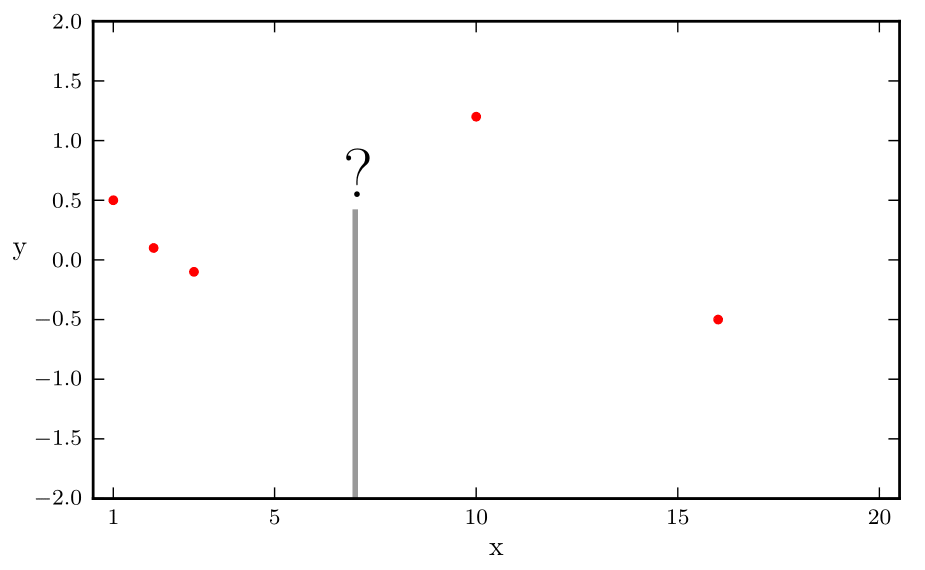
\includegraphics[width=\linewidth]{images/Gaussian process/motivazione2.png}
\end{subfigure}%
\begin{subfigure}{.5\textwidth}
  \centering
  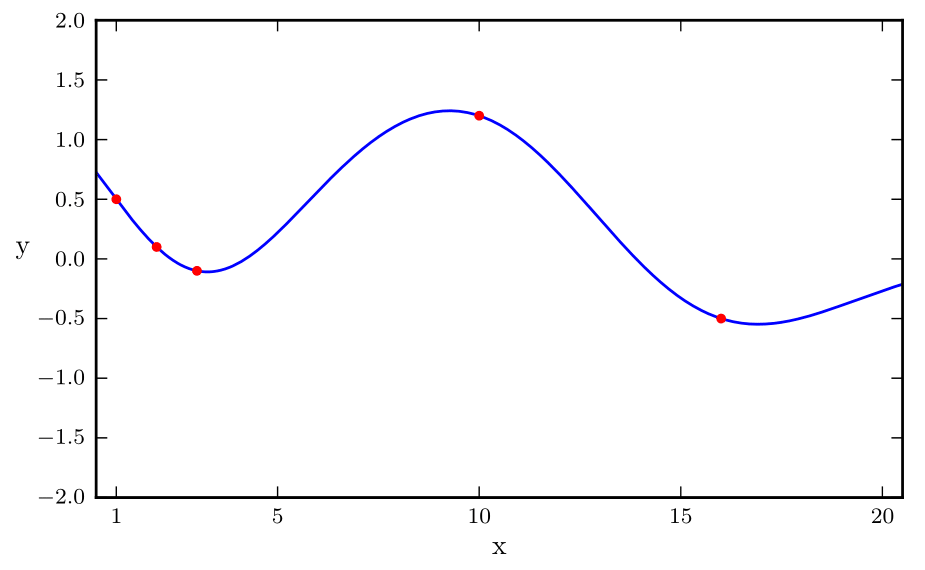
\includegraphics[width=\linewidth]{images/Gaussian process/motivazione3.png}
\end{subfigure}
\caption{Nonlinear regression \cite{turner_gaussian_2016}.}
\end{figure}


\newpage

Gaussian processes provide a good method for the determination of parameters in nonlinear regression not only because they exploit the theory of the multivariate Gaussian distribution, which is overall simple, but because in addition to a function that approximates the data nonlinearly with maximum likelihood (a concept clarified later) they provide an indication of the confidence of the regression in the form of an area within which less likely (but still possible) interpolating functions reside, as illustrated in figure \ref{nonlinearRegressionGaussianProcess}.


%%%%%%%%%%%%%%%%%%%%%%%%%%%%%%%%%%%
%%%%%% IMMAGINE REGRESSIONE NONLINEARE GAUSSIANA
%%%%%%%%%%%%%%%%%%%%%%%%%%%%%%%%%%%
\begin{figure}[h]
    \centering
    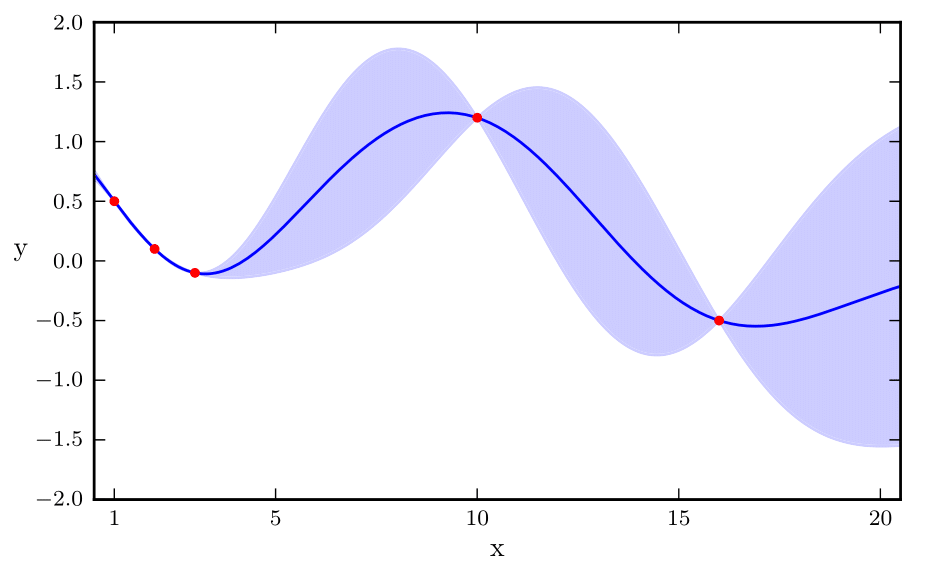
\includegraphics[width=0.85\textwidth]{images/Gaussian process/motivazione4.png}
    \caption{Nonlinear regression with Gaussian processes \cite{turner_gaussian_2016}.}
    \label{nonlinearRegressionGaussianProcess}
\end{figure}

\end{oss}

\newpage

\section{Introduction to Gaussian processes and notation}
Although it is beyond the scope of this paper to go into this in depth, the definition of a stochastic process is given to facilitate the introduction of the notation used.



%%%%%%%%%%%%%%%%%%%%%%%%%%%%
%%%%%% PROCESSO STOCASTICO
%%%%%%%%%%%%%%%%%%%%%%%%%%%%
\begin{defi}[Stochastic process]
  A \textbf{stochastic process} on a probability space $(\Omega, \mathcal{F}, \mathbb{P})$ is a family $\{X_t\}_{t\in T\subset \mathbb{R}}$ of random variables indexed by a parameter $t$.
\end{defi}



It is common to call $t$ the index in order to emphasise the role of time in stochastic processes: a stochastic process generally describes mathematically the temporal evolution of a system characterised by being subject to chance, i.e. a system of which the state at time $t$ cannot be determined with certainty but only by a random variable.\\
In a stochastic system it is therefore only possible to calculate the \textit{probability} that the system is in one of the possible states at time $t>t_0$ if the state at time $t_0$ is known; in a deterministic system, on the other hand, the evolution is described by rules (typically in the form of a differential equation) that allow the state of the system to be precisely determined at each time $t>t_0$ if the state at time $t_0$ is known.




%%%%%%%%%%%%%%%%%%%%%%%%%
%%%%%%% NOTAZIONE
%%%%%%%%%%%%%%%%%%%%%%%%%
\begin{nota}[Functions and indexing in Gaussian processes]
  Writing $f\sim \mathcal{GP}(m,k)$ means that "\textit{ the function $f$ is distributed as a Gaussian process with mean function $m(\cdot)$ and covariance function $k(\cdot,\cdot)$}".\\
  The function thus obtained can be described as:
\[f: \chi \rightarrow \mathbb{R},\]
where $\chi$ is any domain. For each element $x$ in the domain $\chi$ there exists a random variable $f(x)$ with which it is associated.
\end{nota}



\begin{oss}[Versatility of Gaussian processes and generalisation of Gaussian vectors] \label{oss1}
  Note that the domain $\chi$ has no restrictions, a feature that makes Gaussian processes very versatile. Note also that with a finite domain a Gaussian process is a multivariate Gaussian vector. In this sense, as mentioned above, Gaussian processes are a generalisation of multivariate Gaussian vectors. 
\end{oss}


\newpage
%%%%%%%%%%%%%%%%%%%%%
%%%%%% MEAN FUNCTION
%%%%%%%%%%%%%%%%%%%%%
\begin{defi}[Mean function]
Given $f\sim \mathcal{GP}(m,k)$ a Gaussian process, the \textbf{mean function} is a function
\[
m:\chi \rightarrow \mathbb{R}
\]
where $m(x)=\mathbb{E}[f(x)]$.
\end{defi}

\begin{oss}
  For the \textit{mean function} there is no requirement in terms of properties of the function. Typical choices are $m(x)=0$ or $m(x)=c$ with $c$ constant.
\end{oss}

Contrary to \textit{mean function}, the choice of \textit{covariance function} is restricted to a certain class of functions, so some preliminary concepts are introduced before the definition.




%%%%%%%%%%%%%%%%%%%%%%%%
%%%% MERCER KERNEL
%%%%%%%%%%%%%%%%%%%%%%%%
\begin{defi}[Mercer kernel/positive definite kernel]
  A \textbf{Mercer kernel} (or \textbf{positive definite kernel}) is defined as any symmetrical function 
\[
\mathcal{K}: \chi\times\chi \rightarrow \mathbb{R}^+
\]
 such that: $\sum_{i=1}^N\sum_{j=1}^N\mathcal{K}(x_i,x_j)c_ic_j \geq 0$ for any set of distinct elements $\{x_i\}_{i=1}^N\subset \chi$, $\{c_i\}_{i=1}^N\subset  \mathbb{R}$.
\end{defi}

An alternative definition is based on the concept of \textit{Gram matrix}:

\begin{defi}[Gram matrix]
  Given a function $\mathcal{K}: \chi\times \chi\rightarrow \mathbb{R}^+$, let ${x_i}_{i=1}^N\subset \chi$ be any set of distinct elements, we define the \textbf{Gram matrix} of $\mathcal{K}$ to be the following:
\[
\bm{K}=\begin{pmatrix}
    \mathcal{K}(x_1,x_1) & \mathcal{K}(x_1,x_2) & \dots & \mathcal{K}(x_1,x_N)\\
    \mathcal{K}(x_2,x_1) & \mathcal{K}(x_2,x_2) & \dots & \mathcal{K}(x_2,x_N)\\
    \vdots & \vdots & \ddots & \vdots\\
    \mathcal{K}(x_N,x_1) & \mathcal{K}(x_N,x_2) & \dots & \mathcal{K}(x_N,x_N)
    \end{pmatrix}
\]
\end{defi}

\begin{defi}[Mercer kernel/positive definite kernel]
Given a function $
\mathcal{K}: \chi\times\chi \rightarrow \mathbb{R}^+
$, $\mathcal{K}$ is called \textbf{Mercer kernel} if and only if its Gram matrix is positive semidefinite.
\end{defi}

It is now possible to define the covariance function.

\newpage


%%%%%%%%%%%%%%%%%%%%%%%%
%%%% COVARIANCE FUNCTION
%%%%%%%%%%%%%%%%%%%%%%%%
\begin{defi}[Covariance/kernel function]
  Given a Gaussian process $f\sim \mathcal{GP}(m,k)$, the \textbf{covariance function} is a function
\[
k:\chi\times \chi \rightarrow \mathbb{R}
\]
such that $k(\cdot,\cdot)$ is a \textit{Mercer kernel}. The following occurs 
\[k(x,x')=\mathbb{E}[(f(x)-m(x))(f(x')-m(x'))]=\text{Cov}[f(x),f(x')].
\]
\end{defi}

\begin{oss}[Similarity between Gaussian processes and multivariate Gaussian distribution]
  The \textit{mean function} was defined without making any restrictions on the properties of the function, while for the \textit{covariance function} it was required that its Gram matrix be semidefinite positive.\\
  This should come as no surprise: as previously mentioned, Gaussian processes generalise the multivariate Gaussian distribution and as explained in the previous chapter (and emphasised in the remark \ref{ossGaussianaMultivariata}) the latter is defined by two parameters: a mean vector, without any restriction, and a covariance matrix, which must be symmetric and semidefinite positive. There is therefore, in this sense too, similarity between Gaussian processes and multivariate Gaussian distributions.
\end{oss}

\vspace{0.5cm}

%%%%%%%%%%%%%%%%%%%%%%%%%%%%
%%%%%%% ESEMPIO GP
%%%%%%%%%%%%%%%%%%%%%%%%%%%
\begin{ese}[Example of a Gaussian process] \label{esempioProcessoGaussiano}
Consider $f\sim \mathcal{GP}(m,k)$, where:
\[
m(x)=\frac{x^2}{4}\qquad k(x,x')=\text{exp}\left( -\frac{1}{2}(x-x')^2\right).
\]
To understand this example of a Gaussian process, consider the graph of some samples of the function $f$. In order not to work in the infinite case, we consider a finite domain.\footnote{Keep in mind that from a theoretical point of view, the Gaussian processes that are considered in this paper are constructed on an infinite domain of real numbers; however, when generating the graphs, one is forced to consider a finite set of points that are then joined to generate the curve. With this (forced) philosophy, the graphs in the next section are constructed.\label{footnote 1}}: $\chi = \left\{x_i \right\}_{i=1}^{n}$. Since $\chi$ is finite, what is obtained by evaluating $m(\cdot)$ and $k(\cdot,\cdot)$ on the domain are a vector $\bm{\mu}$ and a matrix $\bm{\Sigma}$ where:
\[
\begin{split}
\mu_i&=m(x_i)=\frac{x_i^2}{4} \qquad\qquad\qquad\qquad\qquad\qquad i=1,\dots, n \\
\Sigma_{ij}&=k(x_i,x_j)=\text{exp}\left( -\frac{1}{2}(x_i-x_j)^2\right)\qquad i,j=1,\dots, n
\end{split}
\]
It is thus obtained, as anticipated in the remark \ref{oss1}, that for each $x_i$ in the domain $\chi$ the random variable $f(x_i)$ is a Gaussian random variable of mean $\mu_i$ and variance $\Sigma_{ii}$; calling $\bm{f}=(f(x_1), \dots, f(x_n))^{\text{T}}$ we get, i.e: 
\[
\bm{f}\sim \mathcal{N}(\bm{\mu}, \bm{\Sigma}).
\]

\newpage

Having obtained a multivariate $n$-dimensional Gaussian vector, it is natural to use the same method as introduced in the \ref{sezioneCorrelazione} to derive the graph of the "function" (it is actually a vector) $\bm{f}$. The figure \ref{esempioProcessoGaussianoImmagine} shows the "graphs" of four different samples of a Gaussian vector of dimension $n=60$. Note that the shape of the four graphs is quite different from that of figure \ref{correlazione6} as a consequence of the fact that the distributions have different covariance matrixes. This emphasises how important the covariance function is in Gaussian processes, being responsible for the covariance matrix. This topic will be analysed in detail later.\newline
This example clarified what is meant when it is said that Gaussian processes generalise the multivariate Gaussian distribution.

%%%%%%%%%%%%%%%%%%%%%%%%%
%%%%%%%%% IMMAGINE
%%%%%%%%%%%%%%%%%%%%%%%%
\begin{figure}[h]
    \centering
    \includegraphics[width=0.85\textwidth]{images/Gaussian process/esempioProcessoGaussiano.pdf}
    \caption{Four vectors generated by a Gaussian process defined as in the example \ref{esempioProcessoGaussiano}. Code \ref{Example}.}
    \label{esempioProcessoGaussianoImmagine}
\end{figure}

Note that the code \ref{Example} will not generate the same graph as the figure \ref{esempioProcessoGaussianoImmagine} as there is a random component! The same applies to the other codes mentioned in this chapter.
\end{ese}


\newpage


%%%%%%%%%%%%%%%%%%%%%%%%%%
%%%%% SULLE COVARIANCE FUNCTION
%%%%%%%%%%%%%%%%%%%%%%%%%%


\section{On covariance functions}
For a Gaussian process, the covariance function is of fundamental importance: it is in fact the function $k(\cdot,\cdot)$ that determines how the Gaussian process interprets the data: From the definition of the covariance function, various models can be derived, e.g. linear regression \footnote{Please see \cite{rasmussen_gaussian_2006} and \cite{williams_prediction_1998}} or splines \footnote{Please see \cite{kimeldorf_correspondence_1970}}.\\
\begin{oss}[Importance of covariance]
  In the previous chapter, a visual interpretation of the Pearson correlation index was shown in the \ref{sezioneCorrelazione}, and it was clarified how covariance affects the correlation of two random variables.\\
  Thus, the importance of the covariance function in the correlation between the random variables $f(x)$ and $f(x')$ for each $x,x'\in \chi$ is evident. This is why it is significant, when choosing the covariance function, to take into account how it depends on the pair $(x,x')$.
\end{oss}

Following are the three main types of covariance functions according to their dependence on $(x,x')$ where $x,x'\in \mathbb{R}^D$.




%%%%%%%%%%%%%%%%%%%%%%%%%%
%%%%%%% PROPRIETA KERNEL
%%%%%%%%%%%%%%%%%%%%%%%%%%
\begin{defi}[Stationary covariance function]
  A \textbf{stationary} covariance function is a covariance function that depends on $x-x'$.\\
  A covariance function of this type is translation invariant.
\end{defi}

\begin{defi}[Isotropic covariance function]
  A \textbf{isotropic} covariance function is a covariance function that depends on $|x-x'||$.\\
  Such a covariance function is invariant for rigid motions.
\end{defi}

\begin{defi}[Dot product covariance function]
  A \textbf{dot product} covariance function is a covariance function that depends on $x$ and $x'$ only via $x\cdot x'$.\\
  Such a covariance function is invariant for rotations centred in the origin but not for translations.
\end{defi}

The main covariance functions are shown below. As previously mentioned, this can only be an introduction to the possible choices: important aspects of covariance functions concern their generalisation given by the use of the Mahalanobis distance, a correct choice of kernel for numerical optimisation, relation between kernel choice and deep learning for Gaussian processes \footnote{To further elaborate see \cite{murphy_probabilistic_2022}}, adaptation of kernels to multi-dimensional models \footnote{To further elaborate see \cite{duvenaud_automatic_2014}}...\\
With regard to covariance functions, it is in the interests of this paper to understand how these influence the Gaussian process. Together with the following examples, graphs will therefore be given to support this interest.

\newpage

\subsection{Linear kernel}
%%%%%%%%%%%%%%%%%%%%%%%%%
%%%% LINEAR
%%%%%%%%%%%%%%%%%%%%%%%
\begin{defi}[Linear kernel]
  The \textbf{linear kernel} has the form \[
k(x,x')=\sigma_b^2+\sigma_v^2 (x-c)(x'-c).
\]
\end{defi}

The graph of the function $k(x,x')$ is plotted. A straight line with the usual parameters is obtained.
%%%%%%%%%%%%%%%%%%%%%%%%%
%%%%%%%%% IMMAGINE
%%%%%%%%%%%%%%%%%%%%%%%%
\begin{figure}[h]
    \centering
    \includegraphics[width=0.6\textwidth]{images/Gaussian process/Linear Kernel.pdf}
    \caption{Graph of $k(x,x')$ linear kernel, $\sigma_b^2=1$, $\sigma_v^2=1$, $c=-1$ and $x'=1$. Code \ref{linear kernel code}}
    \label{linear kernel}
\end{figure}

\newpage

Figure \ref{10 sample linear kernel zero mean} shows graphs of functions with distribution $f\sim \mathcal{GP}(m,k)$ where $m(x)=0$ and $k(x,x')$ is the linear kernel, $\sigma_b^2=0$, $\sigma_v^2=1$, $c=0$.



%%%%%%%%%%%%%%%%%%%%%%%%%%%%
%%%%%%%% IMMAGINE
%%%%%%%%%%%%%%%%%%%%%%%%%%%
\begin{figure}[h]
    \centering
    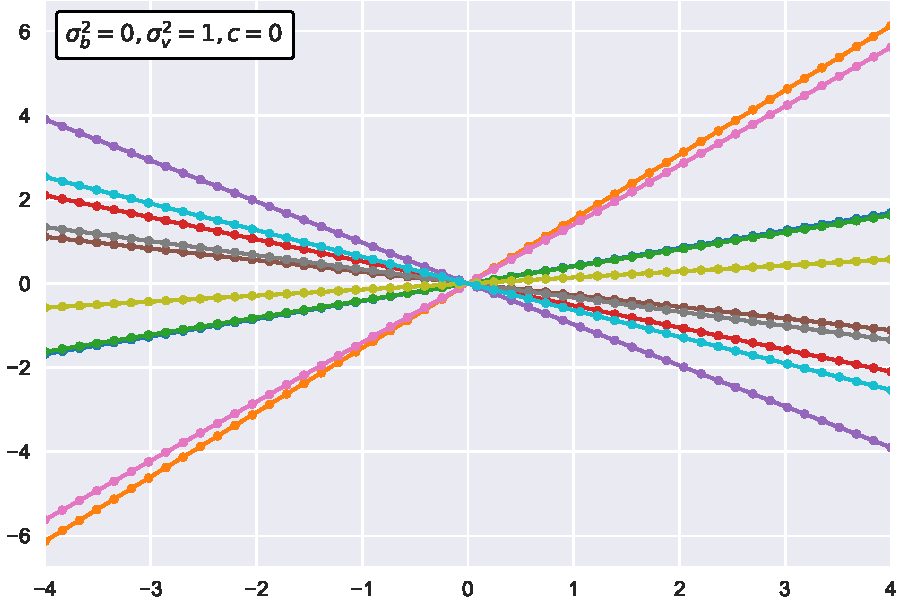
\includegraphics[width=0.85\textwidth]{images/Gaussian process/Linear sample.pdf}
    \caption{Graph of functions with distribution  $f\sim \mathcal{GP}(\bm{0},k)$ where $k(x,x')$ is the linear kernel and $\sigma_b^2=0$, $\sigma_v^2=1$, $c=0$. Code \ref{linear sample}.}
    \label{10 sample linear kernel zero mean}
\end{figure}

Note that the linear kernel generates lines, hence the name.\\
Imposing the mean function equal to zero increases the tendency of lines to pass through the origin. Imposing $m(x)=\alpha\in\mathbb{R}$ increases the tendency of lines to pass through the point $(0,\alpha)$. 
%Esploreremo di seguito l'influenza degli altri parametri del kernel sui grafici delle funzioni, ma è già in parte evidente l'importanza della struttura del kernel nel grafico delle funzioni con distribuzione $\mathcal{GP}(m,k)$.



\newpage






\vspace{1cm}
To understand the influence of parameter $c$, graphs of functions with distribution $f\sim \mathcal{GP}(m,k)$ are shown where $m(x)=0$ and $k(x,x')$ is the linear kernel and the value of $c$ is varied.

%%%%%%%%%%%%%%%%%%%%%%%%%%%%%%%%%%%
%%%%%% IMMAGINI: PARAMETRO c
%%%%%%%%%%%%%%%%%%%%%%%%%%%%%%%%%%%
\begin{figure}[h]
\centering
\begin{subfigure}{.5\textwidth}
  \centering
  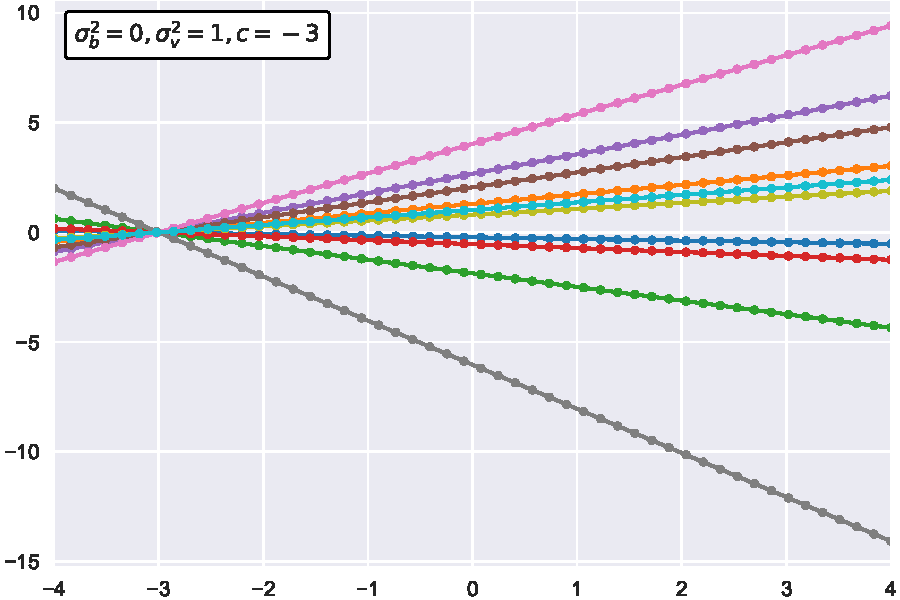
\includegraphics[width=\linewidth]{images/Gaussian process/Linear - c=-3.pdf}
  \caption{$c=-3$}
\end{subfigure}%
\begin{subfigure}{.5\textwidth}
  \centering
  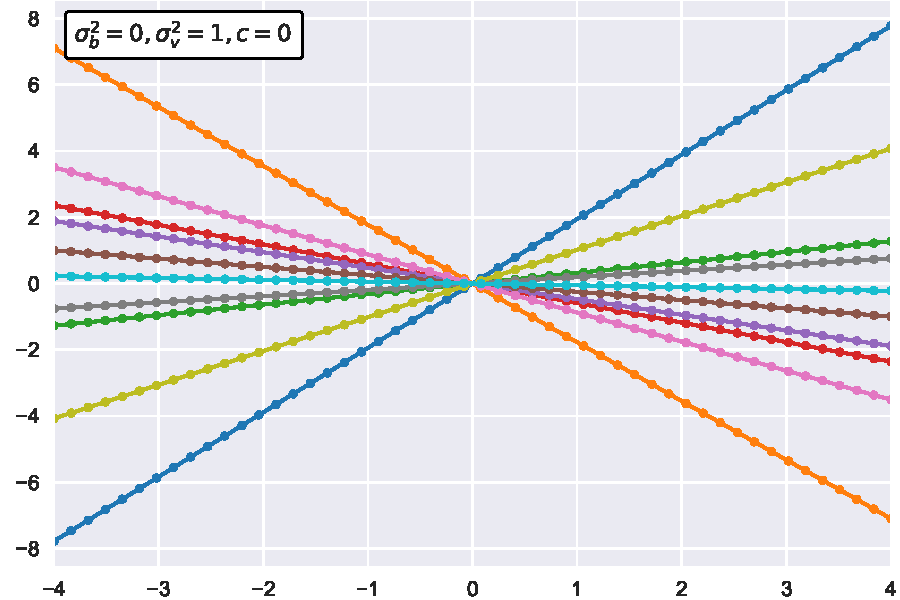
\includegraphics[width=\linewidth]{images/Gaussian process/Linear - c=0.pdf}
  \caption{$c=0$}
\end{subfigure}
\caption{Graph of functions with distribution $f\sim \mathcal{GP}(\bm{0},k)$ where $k(x,x')$ is the linear kernel and $\sigma_b^2=0$, $\sigma_v^2=1$, parameter $c$ is varied. Code \ref{Linear - c}.}
\label{10 sample linear modified c}
\end{figure}


The parameter $c$ therefore imposes a crossing point for all straight lines. Thus $c$ plays the same role as the mean function $m(\cdot)$.

To understand the influence of the parameter $\sigma_b^2$, graphs of functions with distribution $f\sim \mathcal{GP}(m,k)$ are shown where $m(x)=0$ and $k(x,x')$ is the linear kernel and the value of $\sigma_b^2$ is varied.

%%%%%%%%%%%%%%%%%%%%%%%%%%%%%%%%%%%
%%%%%% IMMAGINI: PARAMETRO sigma_b
%%%%%%%%%%%%%%%%%%%%%%%%%%%%%%%%%%%
\begin{figure}[h]
\centering
\begin{subfigure}{.5\textwidth}
  \centering
  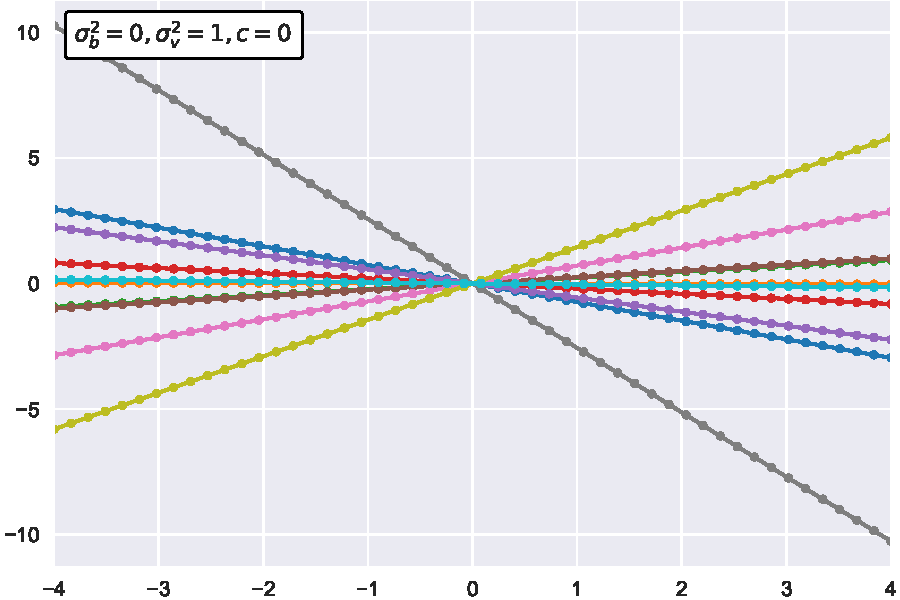
\includegraphics[width=\linewidth]{images/Gaussian process/Linear - sigmab=0.pdf}
  \caption{$\sigma_b^2=0$}
\end{subfigure}%
\begin{subfigure}{.5\textwidth}
  \centering
  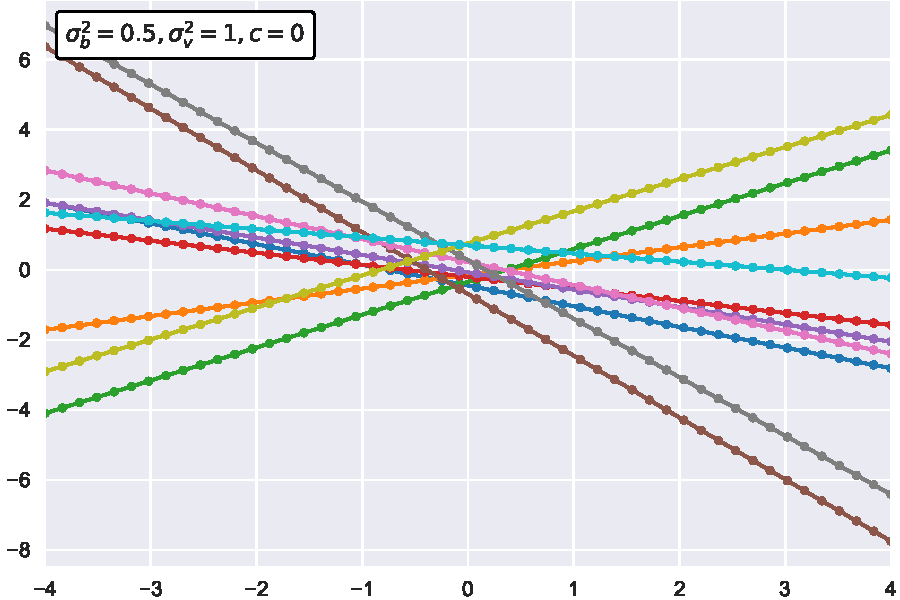
\includegraphics[width=\linewidth]{images/Gaussian process/Linear - sigmab=05.pdf}
  \caption{$\sigma_b^2=0.5$}
\end{subfigure}
\caption{Graph of functions with distribution $f\sim \mathcal{GP}(\bm{0},k)$ where $k(x,x')$ is the linear kernel and $\sigma_v^2=1$, $c=0$, parameter $\sigma_b^2$ is varied. Code \ref{Linear - sigmab}.}
\label{10 sample linear modified sigmab}
\end{figure}
Thus, the parameter $\sigma_b$ influences the precision with which the functions tend to pass through the point $(0,c)$.

\newpage

To understand the influence of the parameter $\sigma_v^2$, graphs of functions with distribution $f\sim \mathcal{GP}(m,k)$ are shown where $m(x)=0$ and $k(x,x')$ is the linear kernel and the value of $\sigma_v^2$ is varied.


%%%%%%%%%%%%%%%%%%%%%%%%%%%%%%%%%%%
%%%%%% IMMAGINI: PARAMETRO sigma_v
%%%%%%%%%%%%%%%%%%%%%%%%%%%%%%%%%%%
\begin{figure}[h]
\centering
\begin{subfigure}{.5\textwidth}
  \centering
  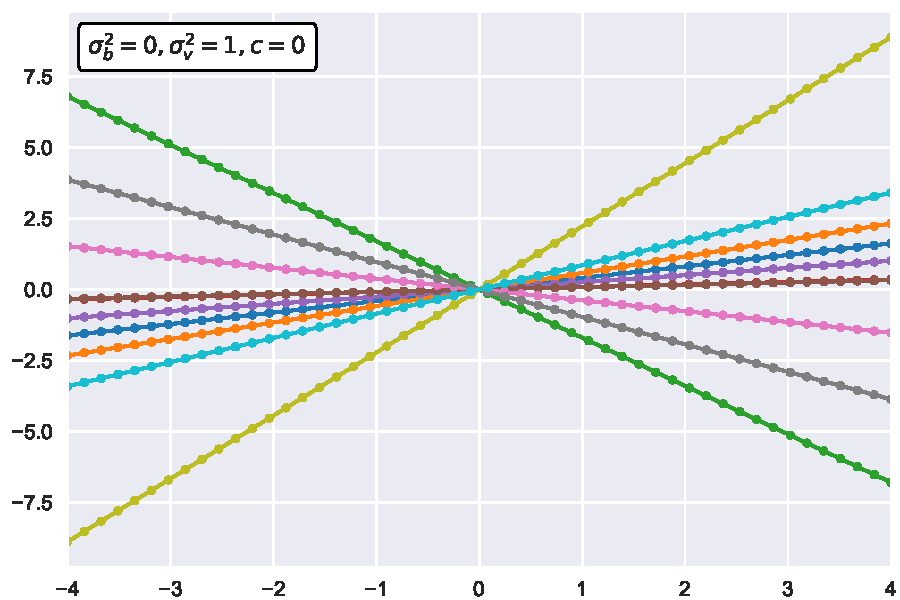
\includegraphics[width=\linewidth]{images/Gaussian process/Linear - sigmav=1.pdf}
  \caption{$\sigma_v^2=1$}
\end{subfigure}%
\begin{subfigure}{.5\textwidth}
  \centering
  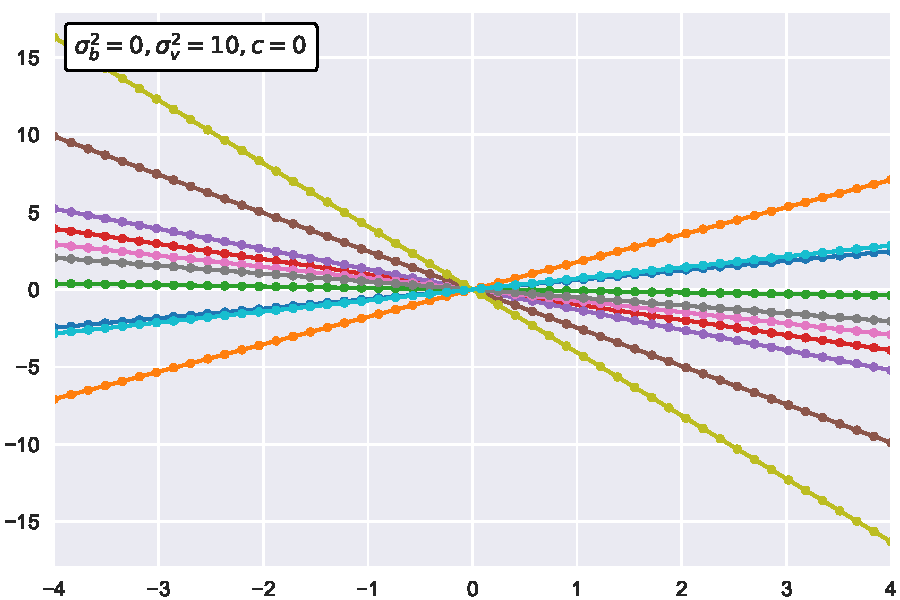
\includegraphics[width=\linewidth]{images/Gaussian process/Linear - sigmav=10.pdf}
  \caption{$\sigma_v^2=10$}
\end{subfigure}
\caption{Graph of functions with distribution $f\sim \mathcal{GP}(\bm{0},k)$ where $k(x,x')$ is the linear kernel and $\sigma_b^2=0$, $c=0$, parameter $\sigma_v^2$ is varied. Code \ref{Linear - sigmav}.}
\label{10 sample linear modified sigmav}
\end{figure}

So the parameter $\sigma_v^2$ influences the slope of the lines, which is proportional to its value.

To understand the influence of the mean function, graphs of functions with distribution $f\sim \mathcal{GP}(m,k)$ where $m(x)=x^3$ and $k(\cdot,\cdot)$ is the linear kernel are shown below.


%%%%%%%%%%%%%%%%%%%%%%%%%%%%
%%%%%%%% IMMAGINE
%%%%%%%%%%%%%%%%%%%%%%%%%%%
\begin{figure}[h]
    \centering
    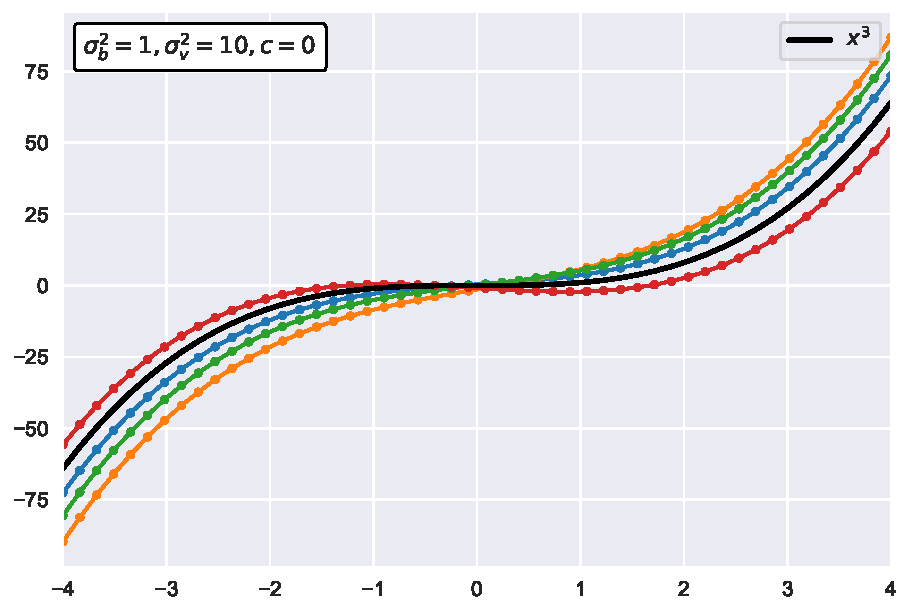
\includegraphics[width=0.85\textwidth]{images/Gaussian process/Linear - cubedmean.pdf}
    \caption{Graph of functions with distribution $f\sim \mathcal{GP}(m,k)$ where $m(x)=x^3$ e $k(x,x')$ is the linear kernel, $\sigma_b^2=1$, $\sigma_v^2=10$, $c=0$. Code \ref{linear cubedmean}.}
    \label{10 sample linear kernel cubed mean}
\end{figure}


\newpage

It is evident from the graph that the graphs resemble the function $x^3$. It will become clearer in the next kernel examples, but from the definition of a Gaussian process (thinking of the multivariate Gaussian distribution, which generalises) every point can be interpreted as a sample of a Gaussian distribution. Recalling the observation \ref{normal decomposition}, we know that every normal (univariate) distribution is decomposable into $Y=\mu+\sigma Z$ where $Z\sim \mathcal{N}(0,1)$; therefore every point $x_i$ on the graph of a function with distribution the Gaussian process as in figure \ref{10 sample linear kernel cubed mean} has decomposition $x_i^3+k(x_i,x_i)Z$. It is therefore clear from the decomposition of each point that the graphs will add to the function $x^3$ an addend due to the covariance function.





\subsection{Squared-exponential kernel}
%%%%%%%%%%%%%%%%
%%% SQUARED-EXPONENTIAL
%%%%%%%%%%%%%


%% A volte è usata ||x-x'||
\begin{defi}[Squared-exponential kernel]
  The \textbf{squared-exponential kernel} has form:
\[
k(x,x')=\sigma^2 \text{exp}\left( -\frac{(x-x')^2}{2l^2} \right).
\]
It is therefore an isotropic covariance function.
\end{defi}

The graph of the function $k(x,x')$ is shown. Note that the parameter $\sigma^2$ affects the peak of the function, while the parameter $l$ affects it indirectly by modifying the rate at which it cancels.



%%%%%%%%%%%%%%%%%%%%%%%%%
%%%%%%%%% IMMAGINE
%%%%%%%%%%%%%%%%%%%%%%%%
\begin{figure}[h]
    \centering
    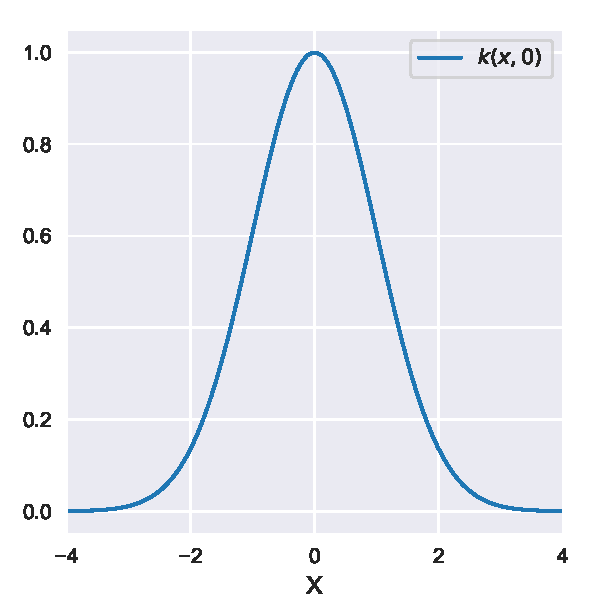
\includegraphics[width=0.6\textwidth]{images/Gaussian process/Squared-exponential kernel.pdf}
    \caption{Graph of $k(x,x')$ squared-exponential kernel, $\sigma^2=1$ and $l^2=1$. Code \ref{squared-exponential}.}
    \label{squared-exponential kernel}
\end{figure}

\newpage

Una funzione distribuita come il processo gaussiano con questo tipo di kernel è $C^\infty$. Esistono diverse variazioni di questo kernel codificanti ipotesi leggermente diverse
A distributed function such as the Gaussian process with this type of kernel is $C^\infty$. There are several variations of this kernel encoding slightly different assumptions about the continuity (even local) of the function, but these are not in the interest of the paper. \footnote{For more details see \cite{duvenaud_automatic_2014}}
\vspace{0.5cm}\\

Shown below are graphs of functions with distribution $f\sim \mathcal{GP}(m,k)$ where $m(x)=0$ and $k(x,x')$ is the squared-exponential kernel.


%%%%%%%%%%%%%%%%%%%%%%%%%
%%%%%%%%% IMMAGINE
%%%%%%%%%%%%%%%%%%%%%%%%
\begin{figure}[h]
    \centering
    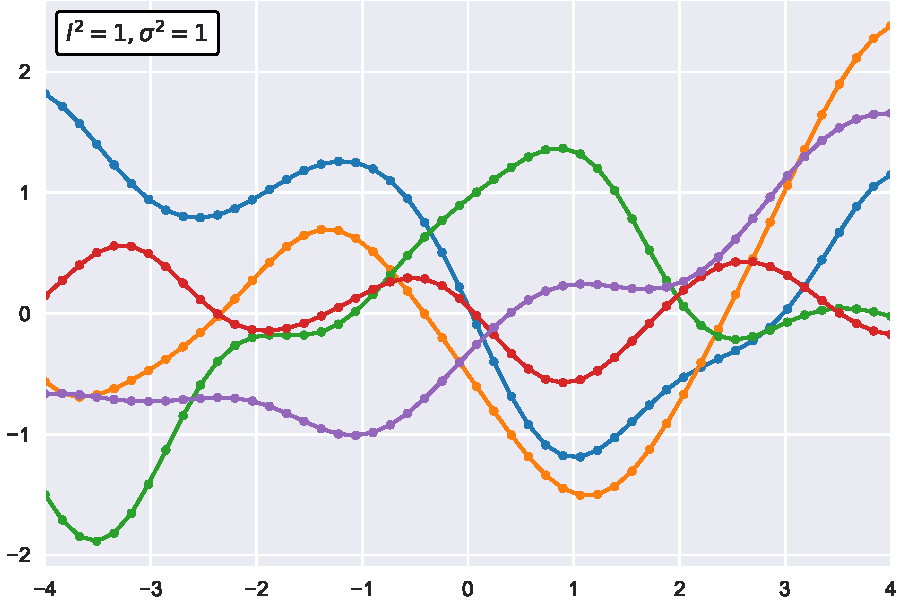
\includegraphics[width=0.85\textwidth]{images/Gaussian process/RBFSample.pdf}
    \caption{Graph of functions with distribution $f\sim \mathcal{GP}(\bm{0},k)$ where $k(x,x')$ is the squared-exponential kernel and $l^2=1$, $\sigma^2=1$. Code \ref{RBF sample}.}
    \label{10 sample exponential kerne zero mean}
\end{figure}

From the figure \ref{10 sample exponential kerne zero mean}, it is possible to see the difference that the kernel has caused in the shape of the function graph: comparing it with the figure \ref{10 sample linear kernel zero mean}, the importance of the choice of kernel according to the context of its use is evident.\\
As in the case of the linear kernel, imposing the mean function at another constant will result in the functions being translated on the $y$-axis.


\newpage 



To understand the influence of the parameter $\sigma^2$, graphs of functions with distribution $f\sim \mathcal{GP}(m,k)$ are shown where $m(x)=0$ and $k(x,x')$ is the squared-exponential kernel, with $l^2=1$ and two different values of $\sigma^2$.
%%%%%%%%%%%%%%%%%%%%%%%%%%%%%%%%%%%
%%%%%% IMMAGINI: PARAMETRO sigma
%%%%%%%%%%%%%%%%%%%%%%%%%%%%%%%%%%%
\begin{figure}[h]
\centering
\begin{subfigure}{.5\textwidth}
  \centering
  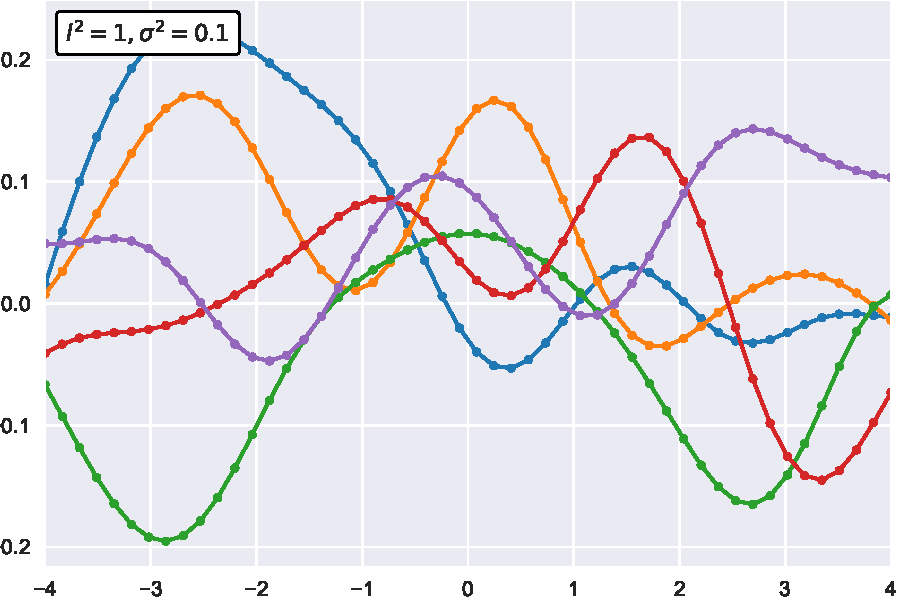
\includegraphics[width=\linewidth]{images/Gaussian process/RBF - sigma=01.pdf}
  \caption{$\sigma^2=0.1$}
\end{subfigure}%
\begin{subfigure}{.5\textwidth}
  \centering
  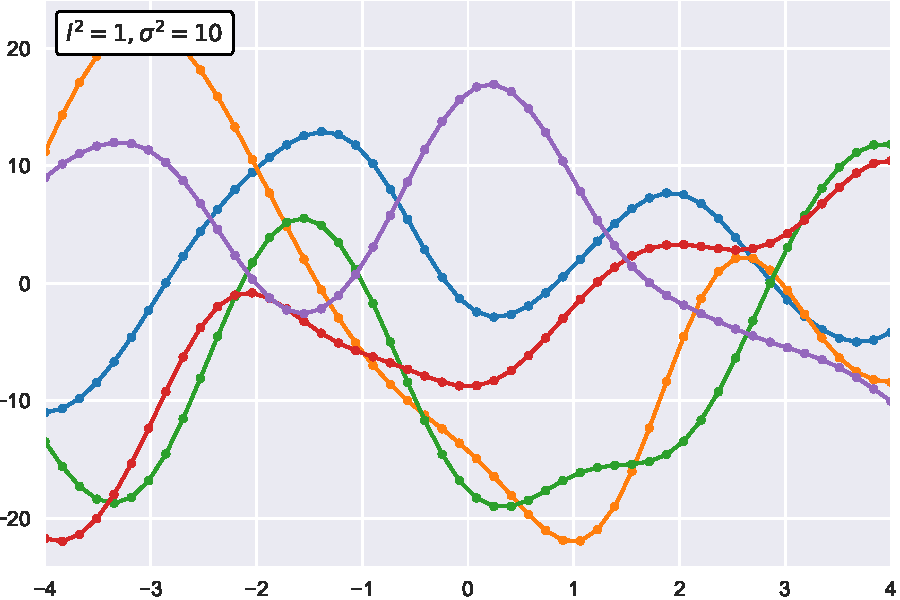
\includegraphics[width=\linewidth]{images/Gaussian process/RBF - sigma=10.pdf}
  \caption{$\sigma^2=10$}
\end{subfigure}
\caption{Graph of functions with distribution $f\sim \mathcal{GP}(\bm{0},k)$ where $k(x,x')$ is the squared-exponential kernel and $l^2=1$, parameter $\sigma^2$ is varied. Code \ref{RBF - sigma}.}
\label{10 sample exponential modified sigma}
\end{figure}

In the two cases, therefore, it changes how far the functions are from the line $x=0$, i.e. proportionally to the value of $\sigma^2$. In reality, $\sigma^2$ affects the tendency of the functions to distance themselves from the mean $m(x)$.

To understand the influence of the parameter $l^2$, graphs of functions with distribution $f\sim \mathcal{GP}(m,k)$ are shown below, where $m(x)=0$ and $k(x,x')$ is the squared-exponential kernel and the parameter $l^2$ is varied.


%%%%%%%%%%%%%%%%%%%%%%%%%%%%%%%%%%%
%%%%%% IMMAGINI: PARAMETRO l
%%%%%%%%%%%%%%%%%%%%%%%%%%%%%%%%%%%
\begin{figure}[h]
\centering
\begin{subfigure}{.5\textwidth}
  \centering
  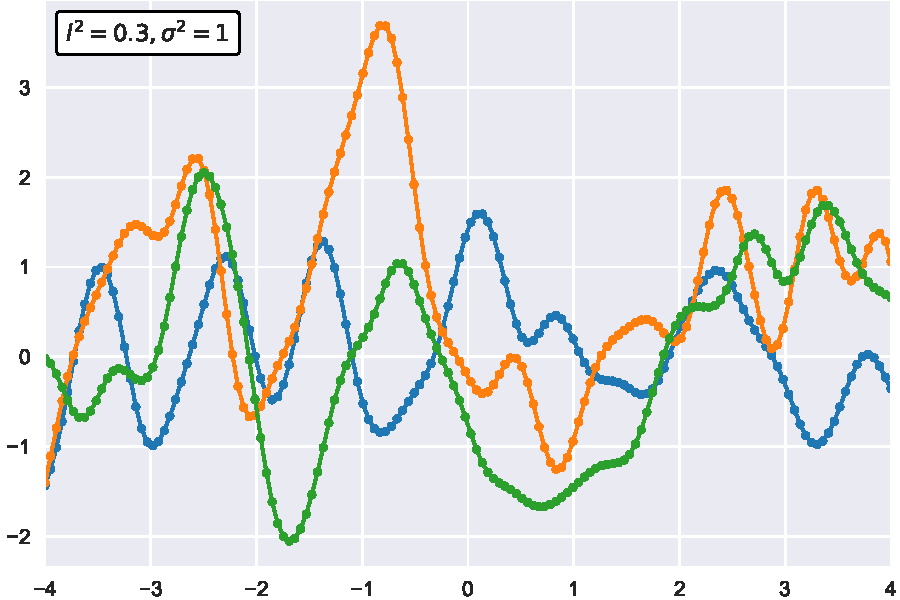
\includegraphics[width=\linewidth]{images/Gaussian process/RBF - l=03.pdf}
  \caption{$l^2=0.3$}
\end{subfigure}%
\begin{subfigure}{.5\textwidth}
  \centering
  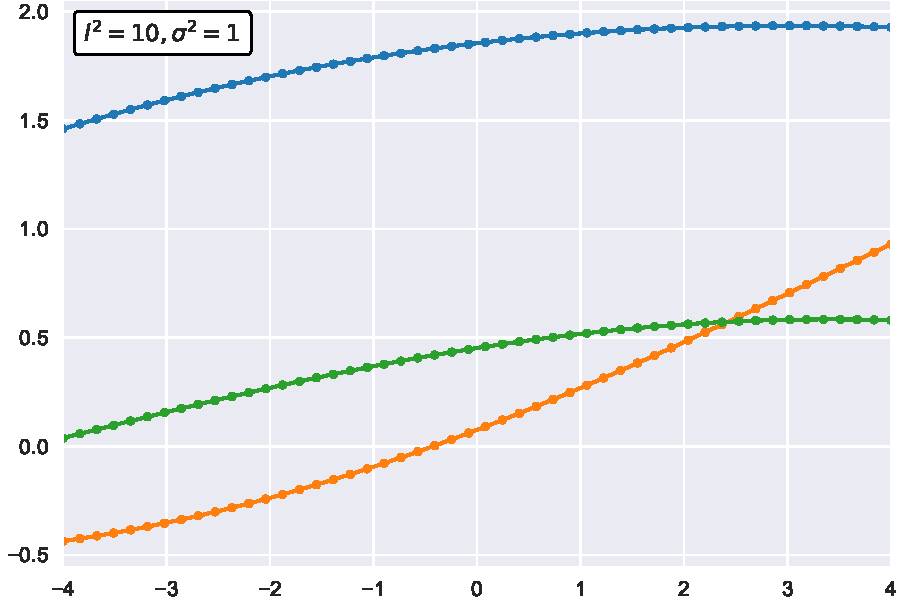
\includegraphics[width=\linewidth]{images/Gaussian process/RBF - l=10.pdf}
  \caption{$l^2=10$}
\end{subfigure}
\caption{Graph of functions with distribution  $f\sim \mathcal{GP}(\bm{0},k)$ where $k(x,x')$ is the squared-exponential kernel and $\sigma^2=1$, parameter $l^2$ is varied. Code \ref{codice9}.}
\label{10 sample exponential modified l}
\end{figure}

The parameter $l^2$ thus modifies the oscillation frequency of the functions.

\newpage

To understand the influence of the mean function, graphs of functions with distribution $f\sim \mathcal{GP}(m,k)$ where $m(x)=x^3$ and $k(x,x')$ the squared-exponential kernel are shown below.
%%%%%%%%%%%%%%%%%%%%%%%%%
%%%%%%%%% IMMAGINE
%%%%%%%%%%%%%%%%%%%%%%%%
\begin{figure}[h]
    \centering
    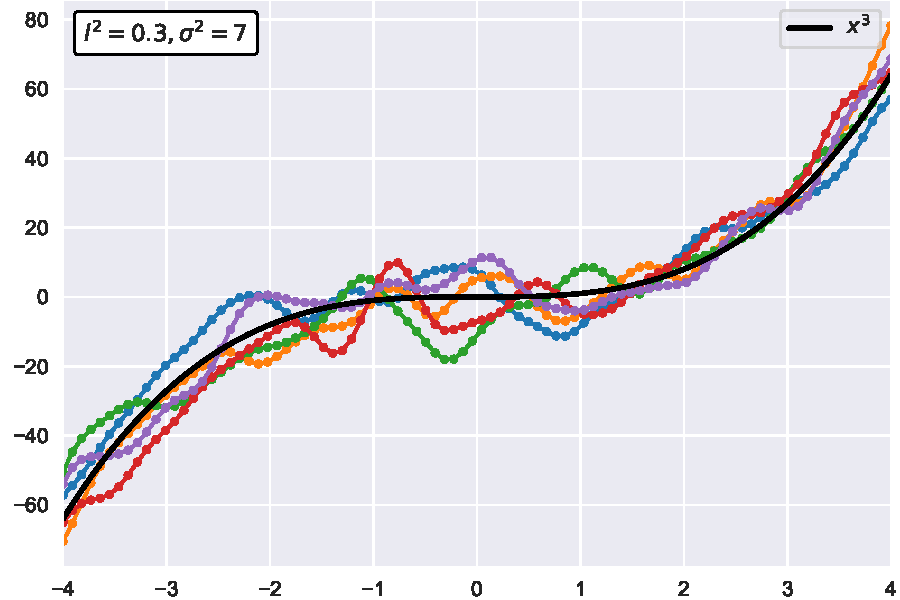
\includegraphics[width=0.85\textwidth]{images/Gaussian process/RBF - cubedmean.pdf}
    \caption{Graph of functions with distribution  $f\sim \mathcal{GP}(m,k)$ where $m(x)=x^3$ e $k(x,x')$ is the squared-exponential kernel, $\sigma^2=7$ and $l=0.3$. Code \ref{codice10}.}
    \label{10 sample exponential kernel cubed mean}
\end{figure}

Parameters have been chosen so that the graphs of the functions stand out. With $\sigma^2=7$ (thus a large distance from the mean function) and $l^2=0.3$ (thus a large oscillation frequency) the functions tend to emulate the mean $m(x)=x^3$ while maintaining the kernel-induced properties.

\newpage








\newpage

\subsection{Periodic kernel}

%%%%%%%%%%%%%%%%%%%%%%%%%%%%
%%%%%%%%% PERIODIC
%%%%%%%%%%%%%%%%%%%%%%%%%%%%
\begin{defi}[Periodic kernel]
  The \textbf{periodic kernel} has form:
\[
k(x,x')=\sigma^2 \text{exp}\left( -\frac{2}{l^2} \text{sin}^2\left( \pi \frac{|x-x'|}{p}\right)\right).
\]
This kernel is therefore also isotropic.
\end{defi}

The graph of the function $k(x,x')$ is shown. Note that the parameter $\sigma^2$ affects the peak of the function as in the \textit{squared-esponential kernel}, similarly the parameter $l^2$ affects the function as in the previous kernel, the parameter $p$ affects the periodicity of the kernel. 


%%%%%%%%%%%%%%%%%%%%%%%%%
%%%%%%%%% IMMAGINE
%%%%%%%%%%%%%%%%%%%%%%%%
\begin{figure}[h]
    \centering
    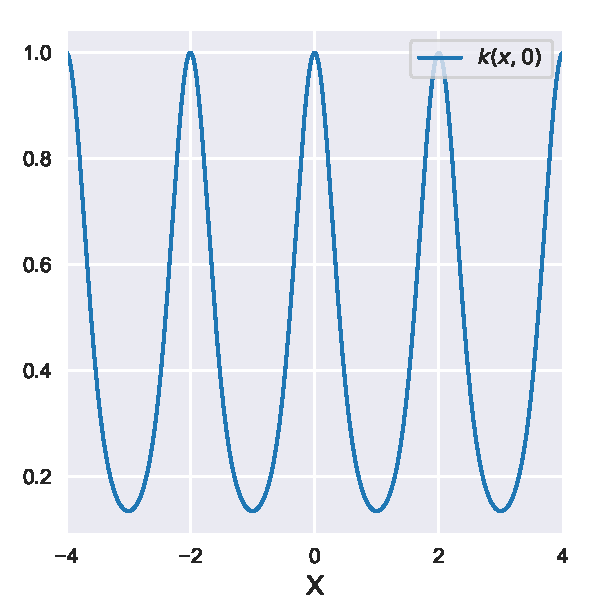
\includegraphics[width=0.6\textwidth]{images/Gaussian process/Periodic kernel.pdf}
    \caption{Graph of $k(x,x')$ periodic kernel, $\sigma^2=1$, $l^2=1$, $p=2$. Code \ref{periodic Kernel}.}
    \label{periodic kernel}
\end{figure}




\newpage
Graphs of functions with distribution $f\sim \mathcal{GP}(m,k)$ where $m(x)=0$ and $k(x,x')$ is the periodic kernel are shown below.

%%%%%%%%%%%%%%%%%%%%%%%%%
%%%%%%%%% IMMAGINE
%%%%%%%%%%%%%%%%%%%%%%%%
\begin{figure}[h]
    \centering
    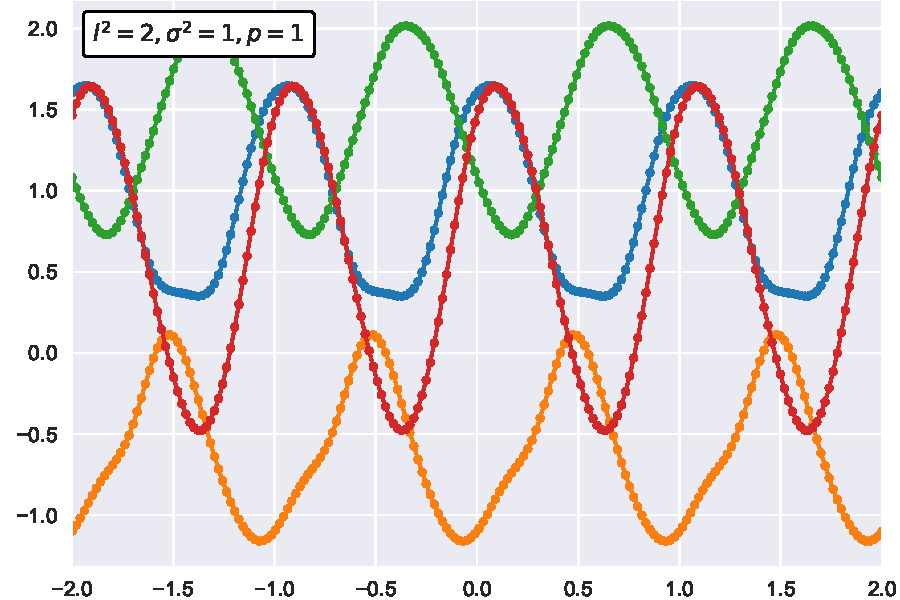
\includegraphics[width=0.85\textwidth]{images/Gaussian process/Periodic sample.pdf}
    \caption{Graph of functions with distribution  $f\sim \mathcal{GP}(\bm{0},k)$ where $k(x,x')$ is the periodic kernel and $\sigma^2=1$, $l^2=2$, $p=1$. Code \ref{periodic sample}.}
    \label{3 sample periodic kerne zero mean}
\end{figure}

As the name of the kernel suggests, the functions are periodic.
To understand the influence of the parameter $\sigma^2$, graphs of functions with distribution $f\sim \mathcal{GP}(m,k)$ where $m(x)=0$ and $k(x,x')$ is the periodic kernel and the parameter $\sigma^2$ is varied are shown below.

%%%%%%%%%%%%%%%%%%%%%%%%%%%%%%%%%%%
%%%%%% IMMAGINI: PARAMETRO sigma
%%%%%%%%%%%%%%%%%%%%%%%%%%%%%%%%%%%
\begin{figure}[h]
\centering
\begin{subfigure}{.5\textwidth}
  \centering
  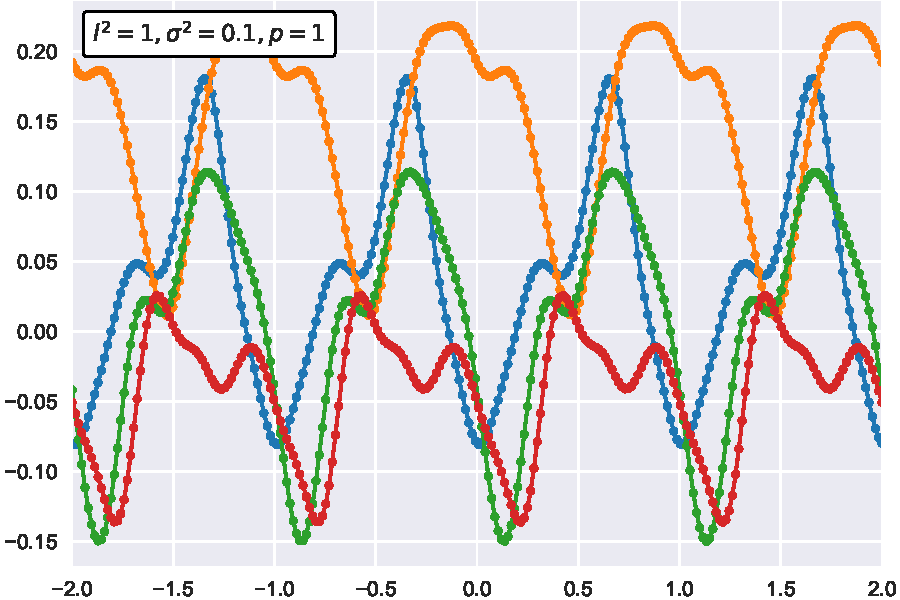
\includegraphics[width=\linewidth]{images/Gaussian process/Periodic - sigma=01.pdf}
  \caption{$\sigma^2=0.1$}
\end{subfigure}%
\begin{subfigure}{.5\textwidth}
  \centering
  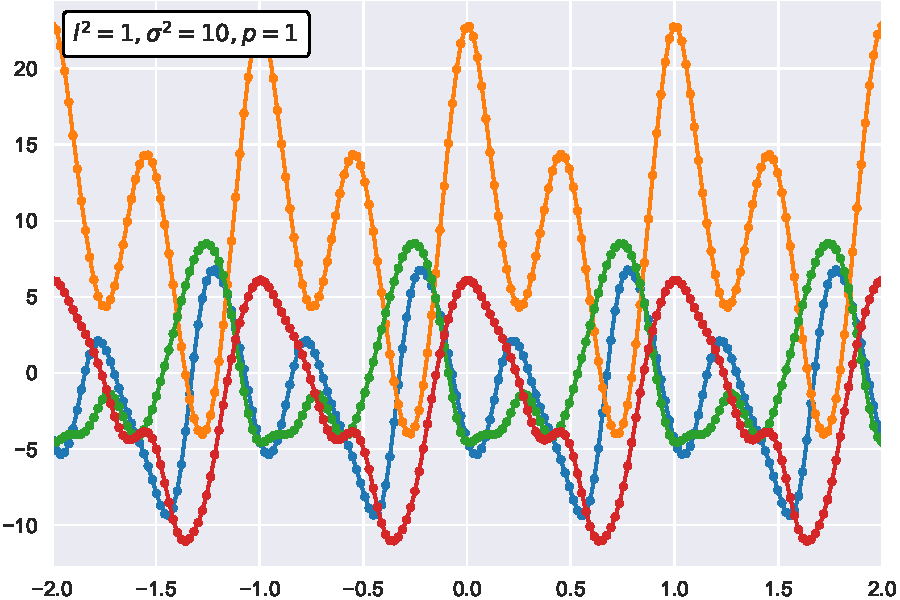
\includegraphics[width=\linewidth]{images/Gaussian process/Periodic - sigma=10.pdf}
  \caption{$\sigma^2=10$}
\end{subfigure}
\caption{Graph of functions with distribution  $f\sim \mathcal{GP}(\bm{0},k)$ where $k(x,x')$ is the periodic kernel and $l^2=1, p=1$, parameter $\sigma^2$ is varied. Code \ref{Periodic sigma}.}
\label{10 sample periodic modified sigma}
\end{figure}

The parameter $\sigma^2$ is thus responsible for the shift of the functions away from the mean, exactly as for the squared-exponential kernel (the figure \ref{10 sample exponential modified sigma} shows similar results).


\newpage

To understand the influence of parameter $p$, graphs of functions with distribution $f\sim \mathcal{GP}(m,k)$ where $m(x)=0$ and $k(x,x')$ is the periodic kernel and parameter $p$ is varied are shown below.

%%%%%%%%%%%%%%%%%%%%%%%%%%%%%%%%%%%
%%%%%% IMMAGINI: PARAMETRO p
%%%%%%%%%%%%%%%%%%%%%%%%%%%%%%%%%%%
\begin{figure}[h]
\centering
\begin{subfigure}{.5\textwidth}
  \centering
  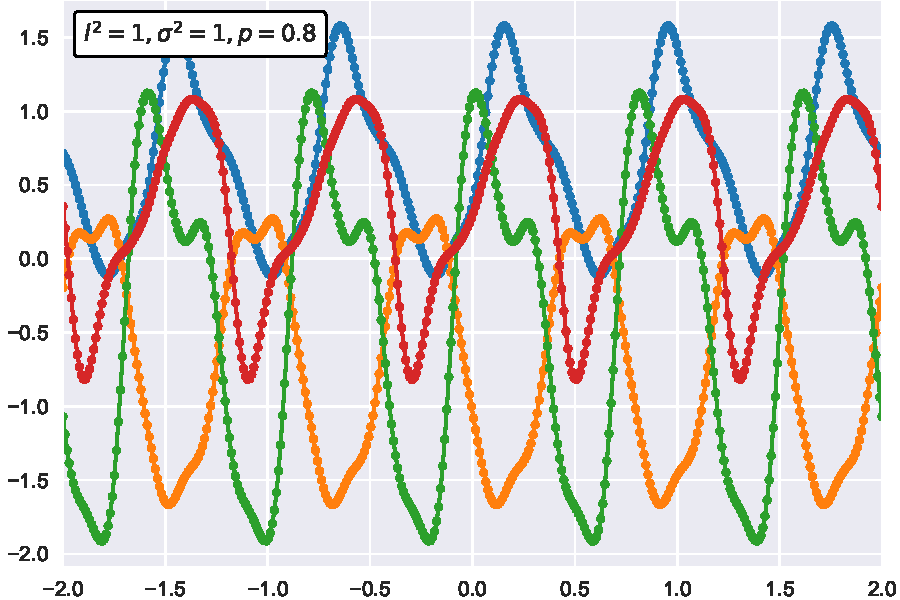
\includegraphics[width=\linewidth]{images/Gaussian process/Periodic - p=08.pdf}
  \caption{$p=0.8$}
\end{subfigure}%
\begin{subfigure}{.5\textwidth}
  \centering
  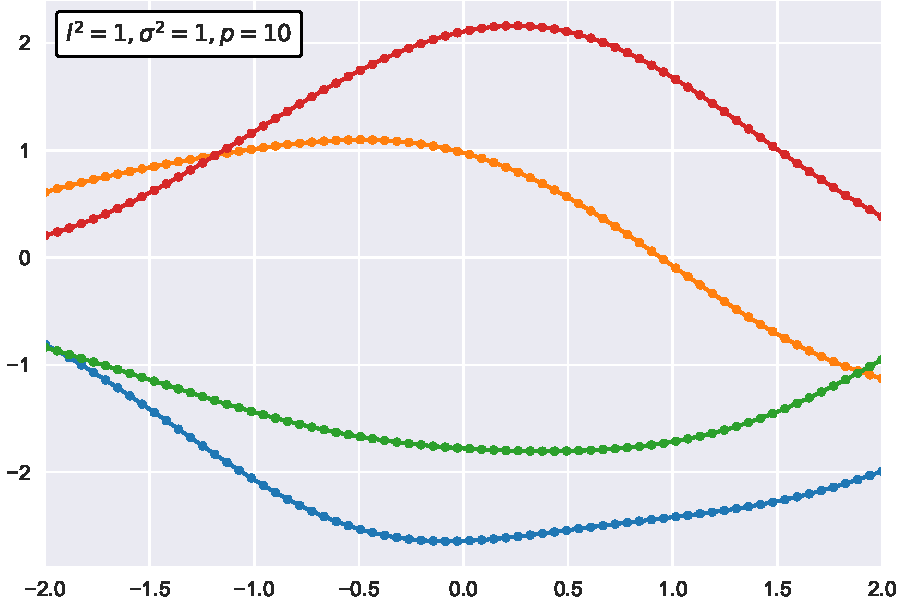
\includegraphics[width=\linewidth]{images/Gaussian process/Periodic - p=10.pdf}
  \caption{$p=10$}
\end{subfigure}
\caption{Graph of functions with distribution  $f\sim \mathcal{GP}(\bm{0},k)$ where $k(x,x')$ is the periodic kernel and $\sigma^2=1$, $l^2=1$ and parameter $p$ is varied. Code \ref{periodic p}.}
\label{10 sample periodic modified p}
\end{figure}

The parameter $p$ thus influences the period of the functions.

To understand the influence of parameter $l^2$, graphs of functions with distribution $f\sim \mathcal{GP}(m,k)$ are shown below, where $m(x)=0$ and $k(x,x')$ is the periodic kernel and parameter $l^2$ is varied.

%%%%%%%%%%%%%%%%%%%%%%%%%%%%%%%%%%%
%%%%%% IMMAGINI: PARAMETRO l
%%%%%%%%%%%%%%%%%%%%%%%%%%%%%%%%%%%
\begin{figure}[h]
\centering
\begin{subfigure}{.5\textwidth}
  \centering
  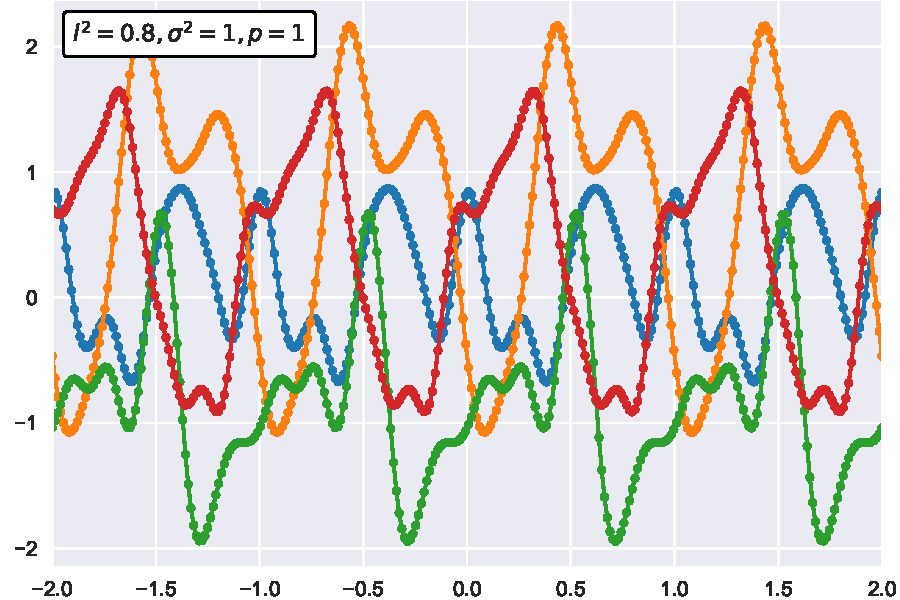
\includegraphics[width=\linewidth]{images/Gaussian process/Periodic - l=0.8.pdf}
  \caption{$l^2=0.8$}
\end{subfigure}%
\begin{subfigure}{.5\textwidth}
  \centering
  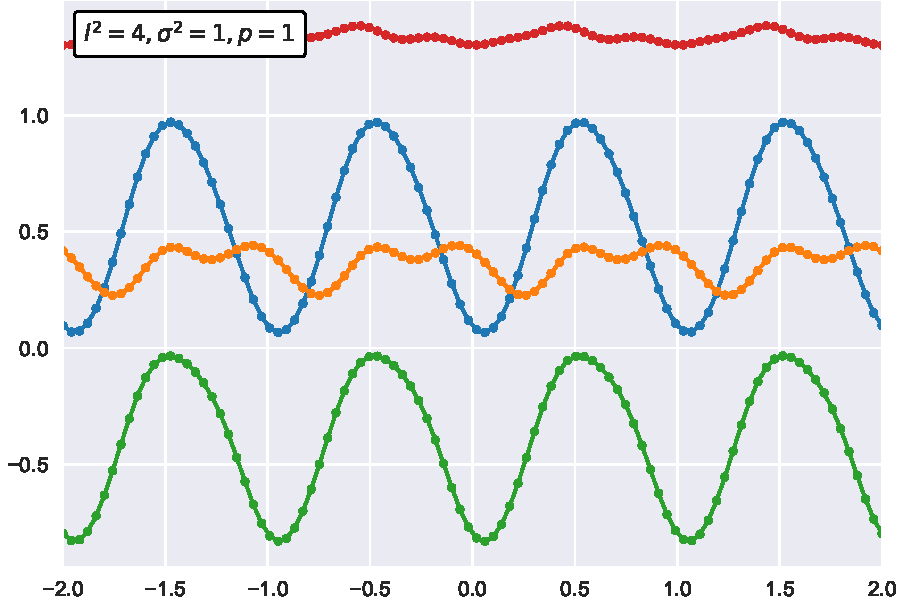
\includegraphics[width=\linewidth]{images/Gaussian process/Periodic - l=4.pdf}
  \caption{$l^2=4$}
\end{subfigure}
\caption{Graph of functions with distribution  $f\sim \mathcal{GP}(\bm{0},k)$ where $k(x,x')$ is the periodic kernel and $\sigma^2=1$, $p=1$ and parameter $l^2$ is varied. Code \ref{periodic l}.}
\label{10 sample periodic modified l}
\end{figure}

The parameter $l^2$ thus influences the 'smoothness' of the frequency of the functions.


\newpage 
To understand the influence of the mean function, graphs of functions with distribution $f\sim \mathcal{GP}(m,k)$ where $m(x)=x^3$ and $k(x,x')$ the periodic kernel are shown below.
%%%%%%%%%%%%%%%%%%%%%%%%%
%%%%%%%%% IMMAGINE
%%%%%%%%%%%%%%%%%%%%%%%%
\begin{figure}[h]
    \centering
    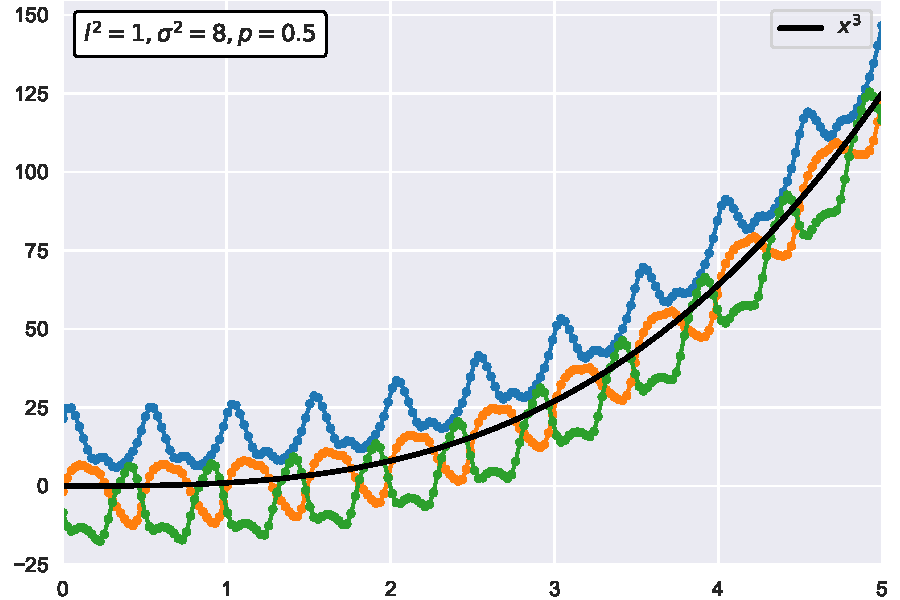
\includegraphics[width=0.85\textwidth]{images/Gaussian process/Periodic - cubedmean.pdf}
    \caption{Graph of functions with distribution  $f\sim \mathcal{GP}(m,k)$ where $m(x)=x^3$ and $k(x,x')$ the periodic kernel, $\sigma^2=8$, $l^2=1$ and $p=0.5$. Code \ref{priodic cubedmean}.}
    \label{3 sample periodic kernel cubed mean}
\end{figure}

Parameters have been chosen so that the graphs of the functions stand out. With $\sigma^2=8$ (thus a large distance from the mean function) and $p=0.5$ (thus a large oscillation frequency) and $l^2=1$ (thus very "angular") the functions tend to emulate the mean $m(x)=x^3$ while maintaining the kernel-induced properties.

\newpage



\subsection{Covariance function in more dimensions}\label{multidimensionalKernel}
One can extend covariance functions in multiple dimensions in various ways. Since the multi-dimensional extension is almost identical for each covariance function, the case of the squared-exponential kernel is shown, as it will be used in the training part of the paper.\\
In order to extend the squared-exponential kernel, it is necessary to extend the subtraction $x-x'$ in more dimensions. The simplest way is to consider the norm $||x-x'||$, a more flexible way is to consider $(x-x')^\text{T}M(x-x')$ where $M$ is a matrix.
This makes it possible to generalise the case:
\[
k(x,x')=\sigma^2 \text{exp}\left( -\frac{||x-x'||^2}{2l^2} \right),
\]
which can be obtained as:
\[
k(x,x')=\sigma^2 \text{exp}\left( -\frac{(x-x')^\text{T}M(x-x')}{2} \right)
\]
imposing $M=l^{-2}I$.\\
The matrix kernel structure allows each dimension to be given a different length scale $l_i$, imposing $M=\text{diag}(\bf{l})^{-2}$, where $\mathbf{l}=(l_1,...,l_n)^\text{T}$. This feature is crucial in training (discussed later in the paper) because if one of these $l_i$ becomes large, the corresponding dimension (which will be seen to correspond to a parameter to be optimised) "loses relevance". The image \ref{multidimensional} provides an example of such behaviour.

%%%%%%%%%%%%%%%%%%%%%%%%%
%%%%%%%%% IMMAGINE
%%%%%%%%%%%%%%%%%%%%%%%%
\begin{figure}[h]
    \centering
    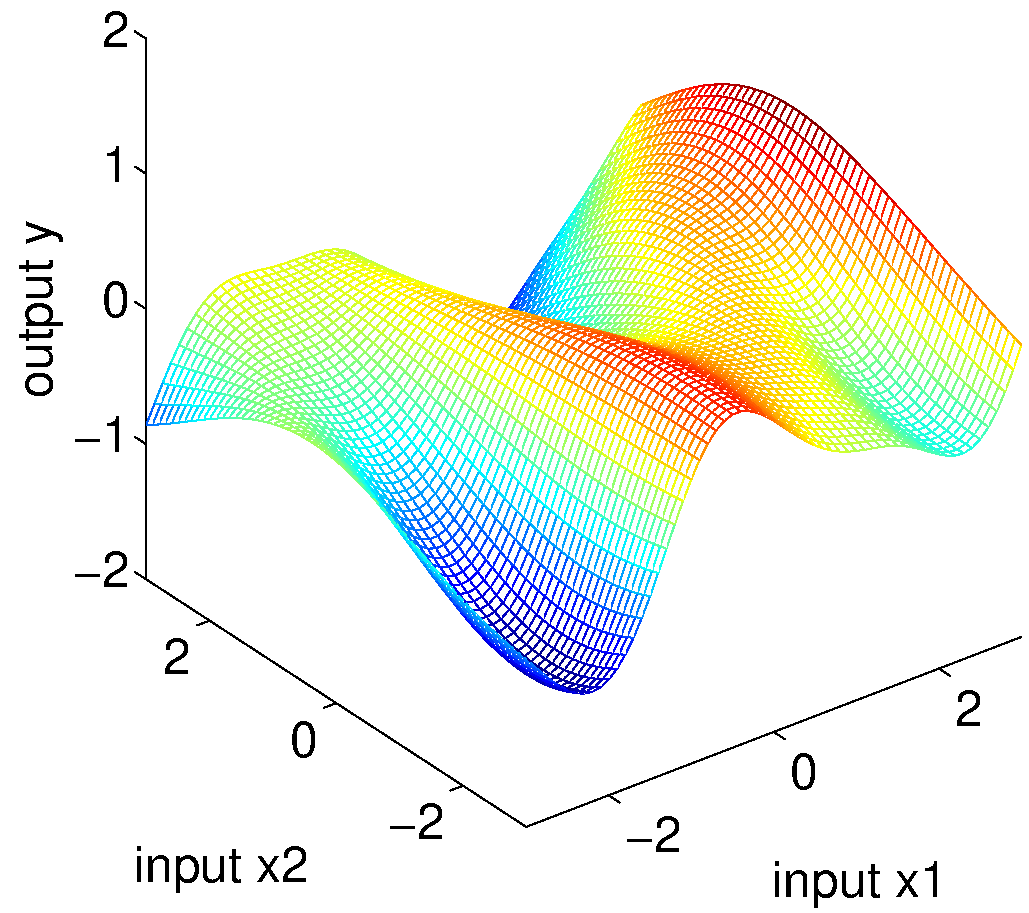
\includegraphics[width=0.6\textwidth]{images/Gaussian process/Multidimensional RBF.pdf}
    \caption{Graph of function with distribution $f\sim \mathcal{GP}(0,k)$ with $k(x,x')$ the squared-exponential kernel in two dimensions in which $M=\text{diag}(1,3)^{-2}$. The function tends to change faster along the $x_1$ direction than along the $x_2$ direction. \cite{murphy_machine_2012}}
    \label{multidimensional}
\end{figure}




\newpage

\subsection{Combining covariance functions}
In the previous sections, the influence of the covariance function on the shape of the function graph has been explained. However, it is not uncommon to have to use functions with shapes other than those imposed by the previously introduced covariance functions. In this case it is possible to construct a new kernel according to the proposition \ref{combining kernel}.


\begin{prop} \label{combining kernel}
  Given two kernels $K_1(x,x')$ and $K_2(x,x')$, by the properties of a kernel the following are still kernels:
\[
\begin{array}{l}
    K(x,x') = c\cdot K_1(x,x') \quad \forall c>0 \text{ costante}\\
    K(x,x') = f(x)K_1(x,x')f(x') \quad \forall f \text{ funzione}\\
    K(x,x') = q(K_1(x,x')) \quad \forall q \text{ funz. polin. a coeff. non negativi}\\
    K(x,x') = \text{exp}(K_1(x,x'))\\
    K(x,x') = K_1(x,x')+K_2(x,x')\\
    K(x,x') = K_1(x,x')\times K_2(x,x')\\
\end{array}
\]
\end{prop}
It is not in the interests of the paper to study in depth the possible combinations of kernels introduced; however, two simple cases of kernel combinations are given for illustrative purposes only.

\newpage




\subsubsection{Squared exponential + periodic kernel}


%%%%%%%%%%%%%%%%%%%%%%%%%
%%%%%%%%% IMMAGINE
%%%%%%%%%%%%%%%%%%%%%%%%
\begin{figure}[h]
    \centering
    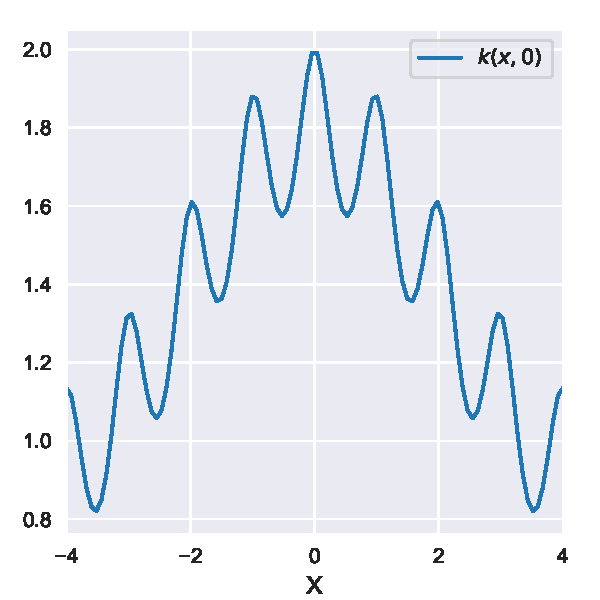
\includegraphics[width=0.55\textwidth]{images/Gaussian process/RBF + periodic kernel.pdf}
    \caption{Graph of $k(x,x')$ squared-exponential kernel summed to periodic kernel. $\sigma^2=1$, $l=2$, $p=1$. Code \ref{RBF + periodic kernel}.}
    \label{SE + periodic kernel}
\end{figure}



%%%%%%%%%%%%%%%%%%%%%%%%%
%%%%%%%%% IMMAGINE
%%%%%%%%%%%%%%%%%%%%%%%%
\begin{figure}[h]
    \centering    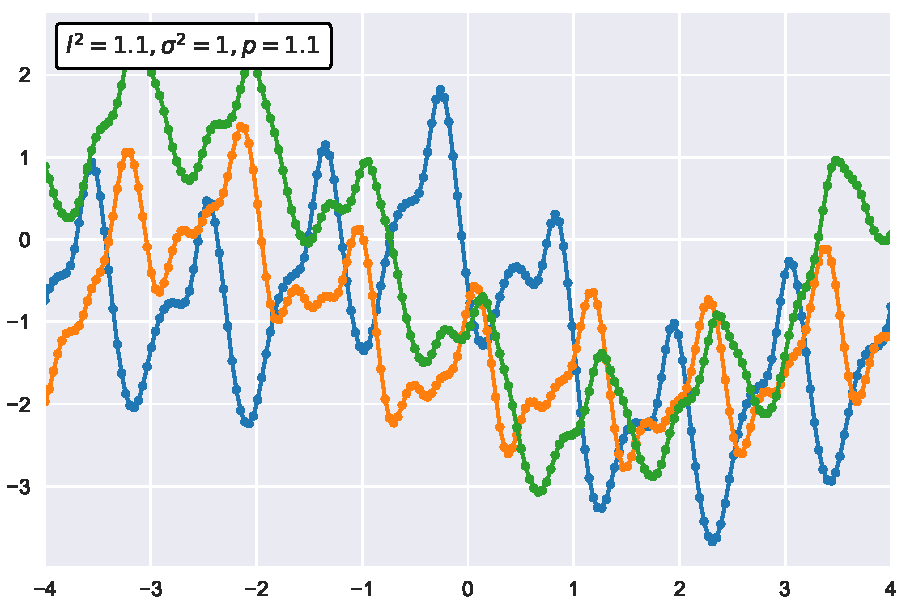
\includegraphics[width=0.69\textwidth]{images/Gaussian process/RBF + periodic sample.pdf}
    \caption{Graph of functions with distribution  $f\sim \mathcal{GP}(\bm{0},k)$ where $k(x,x')$ is the squared-exponential summed to periodic kernel and $l^2=1.1$, $\sigma^2=1$, $p=1.1$. Code \ref{RBF + periodic sample}.}
    \label{SE + periodic sample}
\end{figure}

Combining the two kernels therefore generates periodic functions with perturbations on the pair of axes.

\newpage

\subsubsection{Linear $\times$ linear kernel}

%%%%%%%%%%%%%%%%%%%%%%%%%
%%%%%%%%% IMMAGINE
%%%%%%%%%%%%%%%%%%%%%%%%
\begin{figure}[h]
    \centering
    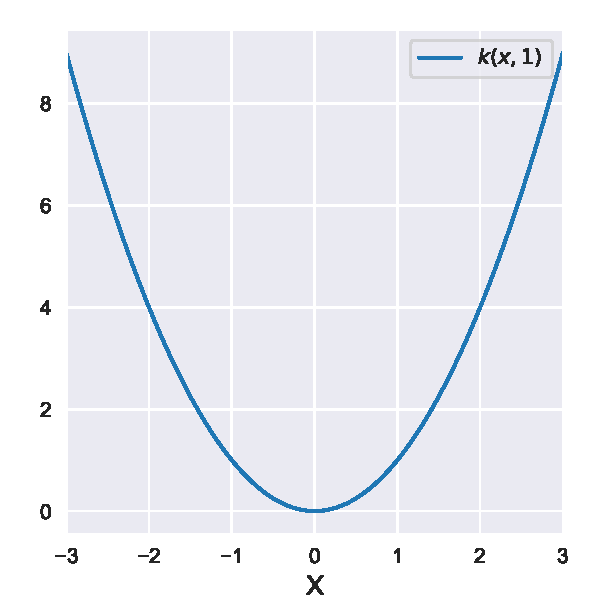
\includegraphics[width=0.55\textwidth]{images/Gaussian process/Linear x Linear kernel.pdf}
    \caption{Graph of $k(x,x')$ linear kernel multiplied by linear kernel. $\sigma_b^2=0$, $\sigma_v^2=1$, $c=0$, $x'=1$. Code \ref{linear x linear}.}
    \label{linear * linear kernel}
\end{figure}


%%%%%%%%%%%%%%%%%%%%%%%%%
%%%%%%%%% IMMAGINE
%%%%%%%%%%%%%%%%%%%%%%%%
\begin{figure}[h]
    \centering
    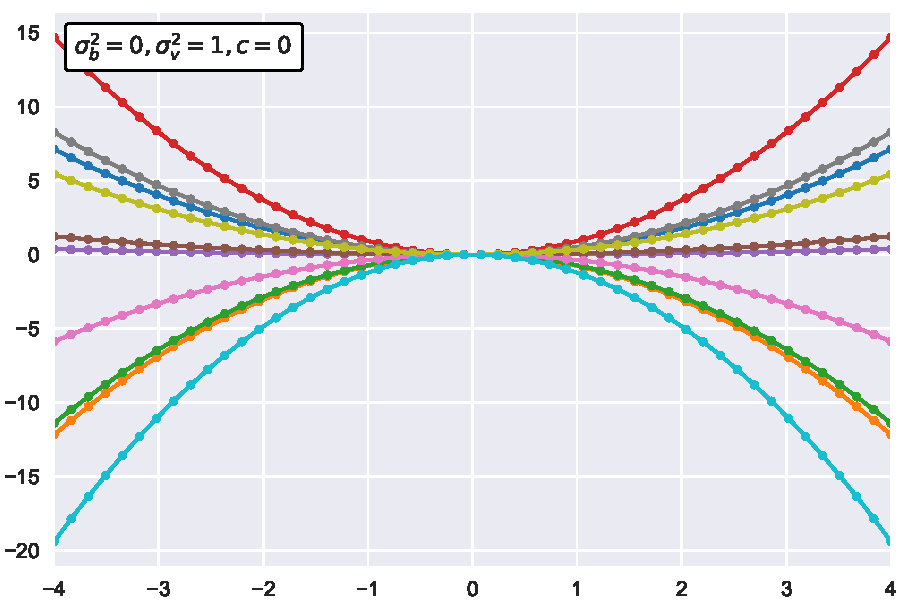
\includegraphics[width=0.68\textwidth]{images/Gaussian process/linear x linear sample.pdf}
    \caption{Graph of functions with distribution  $f\sim \mathcal{GP}(\bm{0},k)$ where $k(x,x')$ is the linear kernel multiplied by linear kernel and $\sigma_b^2=0$, $\sigma_v^2=1$, $c=0$. Code \ref{linear x linear sample}.}
    \label{linear * linear sample}
\end{figure}


Combining the two kernels therefore generates functions with parabolic behaviour. In a sense, it was possible to predict this result by remembering that the linear kernel generates straight lines.

\newpage



\subsubsection{Real-life example of a compound covariance function}\label{section: mauna loa}
It is taken from \cite{rasmussen_gaussian_2006} an example of a regression in which several kernel functions need to be composed.  The data consist of monthly mean atmospheric $CO_2$ concentrations (in parts per million volume: $ppmv$) derived from air samples collected at the Mauna Loa Observatory in Hawaii between 1958 and 2003 (with some missing values). The objective is to model the concentration of $CO_2$ as a function of time $x$, i.e. to predict what is known as \textit{Keeling's curve}. From the figure \ref{CO2}, some features are evident: a long-term increasing trend, a pronounced seasonal variation and some minor irregularities. 


%%%%%%%%%%%%%%%%%%%%%%%%%
%%%%%%%%% IMMAGINE
%%%%%%%%%%%%%%%%%%%%%%%%
\begin{figure}[ht]
    \centering
    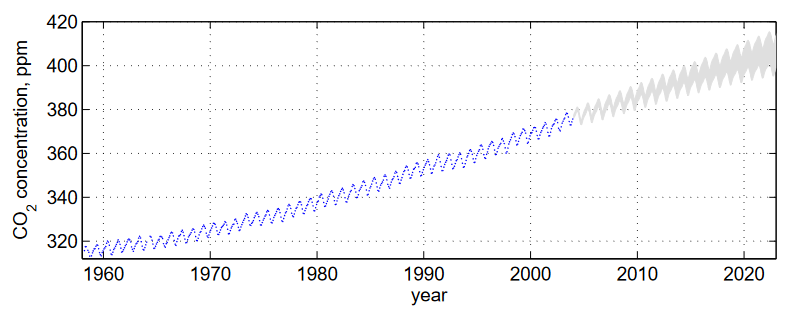
\includegraphics[width=1\textwidth]{images/Gaussian process/Co2_example.PNG}
    \caption{545 observations of monthly averages of the atmospheric concentration of $CO_2$ between 1958 and 2003, the $95\%$ confidence region for a 20-year Gaussian process regression model in the future is also shown. \cite{rasmussen_gaussian_2006}}
    \label{CO2}
\end{figure}


A squared-exponential kernel is used to model the regular and increasing long-term trend:
\[
k_1(x,x')=\theta_1^2\text{exp}\left(-\frac{(x-x')^2}{2\theta_2^2}\right).
\]


The periodic kernel with a period of one year is used to model seasonal variation. Since the seasonal trend is not exactly periodic, the product with a squared-exponential kernel is considered to allow for a decay that is not exactly periodic: 
\[
k_2(x, x') = \theta^2_3 \text{exp}\left( - \frac{(x - x')^2}{2\theta^2_4} - \frac{2 \text{sin}^2(\pi(x - x'))}{\theta^2_5} \right).
\]
A \textit{rational quadratic} kernel is used to model the (small) medium-term irregularities (not introduced in the paper): 
\[
k_3(x, x') = \theta^2_6 \left( 1 + \frac{(x - x')^2}{2\theta_8\theta^2_7} \right)^{-\theta_8}.
\] 
Finally, noise is modelled as the sum of a squared-exponential contribution and an independent component:
\[
k_4(x_p, x_q) = \theta^2_9 \text{exp}\left( \frac{- (x_p - x_q)^2}{2\theta^2_{10}} \right) + \theta^2_{11} \delta_{pq}.
\]

The overall kernel results:
\[
k(x,x')=k_1(x,x')+k_2(x,x')+k_3(x,x')+k_4(x,x'),
\]
where we have $\bm{\theta}=(\theta_1,...,\theta_{11})$ hyperparameters\footnote{see \ref{gerarchica}.}. After a training phase of the model, values are given to the $\theta_i$\footnote{It is explained how this is done in the chapter \ref{machineLearning}.}. Figure \ref{CO2} shows how the model predicts the trend of the atmospheric concentration of $CO_2$ over the twenty years since the last measurement, also showing the ninety-five per cent confidence region. It can be seen that the further one goes in time, the wider the confidence region becomes.\\
Intuitively, the model seems to follow the trend of the graph well, although as the years go by, the region of uncertainty becomes larger, informing little about the actual concentration of $CO_2$. Figure \ref{CO2_comparison} compares the model's prediction with actual data taken from the \href{https://gml.noaa.gov/ccgg/trends/}{Global Monitoring Laboratory}.


%%%%%%%%%%%%%%%%%%%%%%%%%
%%%%%%%%% IMMAGINE
%%%%%%%%%%%%%%%%%%%%%%%%
\begin{figure}[h]
    \centering
    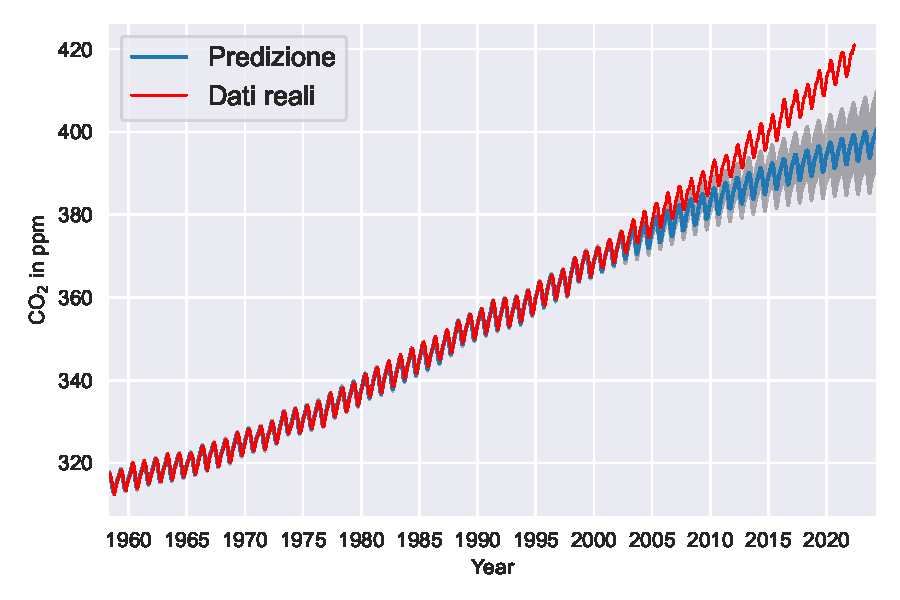
\includegraphics[width=1\textwidth]{images/Gaussian process/MaunaLoaPrediction.pdf}
    \caption{Comparison of the prediction of $CO_2$ concentration with actual data until May 2022.}
    \label{CO2_comparison}
\end{figure}

\newpage

We can therefore see that the forecast was conservative in the long term: the large increase in the concentration of $CO_2$ is due, according to some sources, to how the flora has responded to climate change (drought and precipitation mainly), but also to the large emissions due to the use of fossil fuels.

In a way, therefore, it is reasonable that the prediction is not accurate in recent years as it should have predicted events (from climate change to different rates of fuel consumption) that were not present in the years when the Gaussian process 'learned'.

In figure \ref{CO2_comparison_zoomed}, the previous image from 1995 to 2022 is enlarged, thus emphasising the time period predicted by the Gaussian process.

It can be seen that after 2003, the prediction is rather inaccurate, failing to keep up with rapid human changes (in terms of pollution).  

%%%%%%%%%%%%%%%%%%%%%%%%%
%%%%%%%%% IMMAGINE
%%%%%%%%%%%%%%%%%%%%%%%%
\begin{figure}[h]
    \centering
    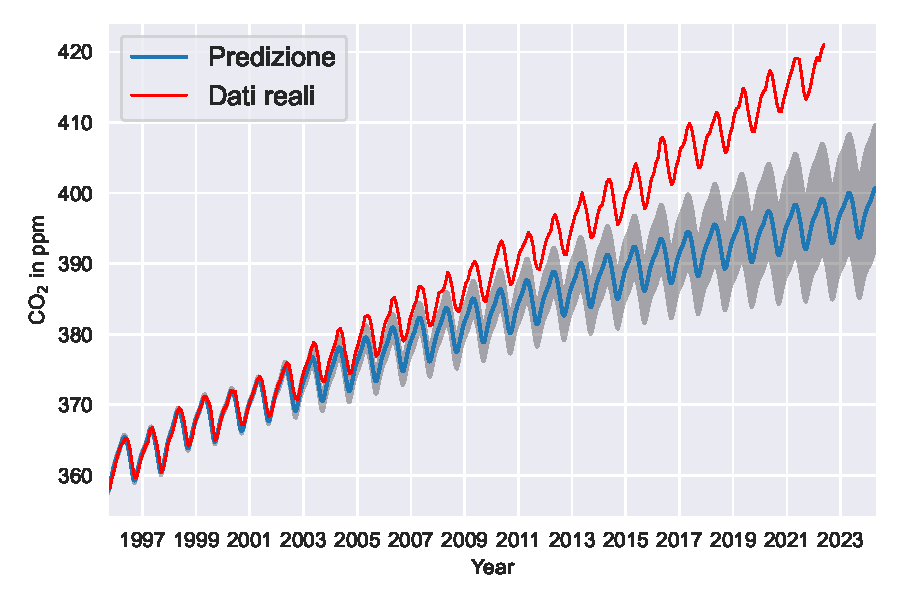
\includegraphics[width=1\textwidth]{images/Gaussian process/MaunaLoaPredictionZoom.pdf}
    \caption{Comparison of the prediction of $CO_2$ concentration with actual data up to 1995 to May 2022.}
    \label{CO2_comparison_zoomed}
\end{figure}




\newpage



\section{Predictions with noiseless observations}\label{regressioneGP}
This section explains how to exploit the information provided by \textit{training data} to generate a function that incorporates a priori knowledge in the case of observations without noise. \\


\begin{defi}[Noise-free training set]
  The \textbf{noise-free training set} is the set of observations \textit{noise-free} defined as: $ \mathcal{D}=\{ (x_n,y_n) : n=1,...,N\}$ where $y_n=f(x_n)$ is the observed value of the function $f$ at point $x_n$. 
\end{defi}


The purpose of the (noise-free) training set is to define a set of points $\mathcal{P}=\{x_n: n=1,...,N\}$ of which the value of the function is known in order to require the Gaussian process to generate functions that interpolate this set of points (i.e. that have value $y_n$ on every $x_n \in \mathcal{P}$ without uncertainty).

\begin{defi}[Test set]
  the \textbf{test set} is the set of values $X_*=\{x_n:n=1,...,N^*\}$ of which the prediction, i.e. the output of the function, is desired.
\end{defi}

Pragmatically, what is being done by defining the \textit{training set} $\mathcal{D}$ is to add the points of $\mathcal{P}$ to the set of points on which to evaluate the covariance function to construct the covariance matrix\footnote{As mentioned in \ref{footnote 1}, to obtain a graph it is necessary to start from a finite domain. This is why we speak of \textit{covariance matrix}.}. Through the conditioning process we obtain the \textit{a posteriori} distribution, that is, the distribution of the functions that interpolate the points of the training set, as illustrated in Figure \ref{intuitiveExplanationOfConditioning}.


%%%%%%%%%%%%%%%%%%%%%%%%%
%%%%%%%%% IMMAGINE
%%%%%%%%%%%%%%%%%%%%%%%%
\begin{figure}[h]
    \centering
    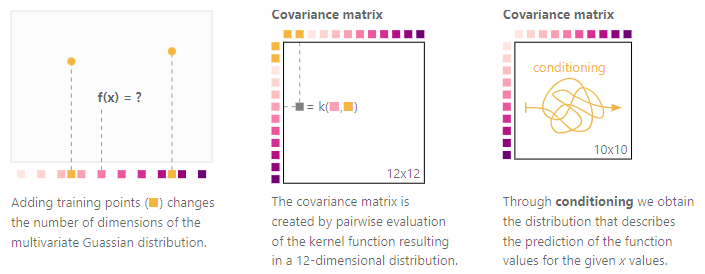
\includegraphics[width=1\textwidth]{images/Gaussian process/GPposterior.PNG}
    \caption{Graphical explanation of how a priori knowledge is incorporated \cite{gortler_visual_2019}.}
    \label{intuitiveExplanationOfConditioning}
\end{figure}

\newpage
Consider now a function distributed as $f\sim \mathcal{GP}(m,k)$. 
Consider now $X^*=\{x_i^*:i=1,\dots,N^*\}$ a \textit{test set} Of which you want to predict the outputs $\bm{f^*}=\left[f(x^*_1), \dots, f(x^*_{N^*}) \right]$; Let also  $\bm{f}=\left[f(x_1), \dots, f(x_N) \right]$ the outputs of the training set where $x_i\in \mathcal{P}$. Recalling that the outputs of the function $f$ follow a Gaussian distribution, the joint distribution can be derived:
\[
\begin{pmatrix}
\bm{f}\\
\bm{f^*}
\end{pmatrix}
=
\mathcal{N}\left(
\begin{pmatrix}
\bm{\mu}\\
\bm{\mu_*}
\end{pmatrix},
\begin{pmatrix}
\bm{K}_{X,X} & \bm{K}_{X,X^*}\\
\bm{K}_{X^*,X} & \bm{K}_{X^*,X^*}
\end{pmatrix}
\right)
\]

where $\bm{\mu}=\begin{pmatrix}m(x_1) \\ \vdots \\ m(x_N)\end{pmatrix}$, $\bm{\mu_*}=\begin{pmatrix}m(x^*_1) \\ \vdots \\ m(x^*_{N^*})\end{pmatrix}$, $\bm{K}_{X,X}=k(X,X)$ is a $N\times N^*$ matrix, $\bm{K}_{X,X^*}=k(X,X^*)$ is a $N\times N^*$ matrix, $\bm{K}_{X^*,X}=k(X^*,X)$ is a $N^*\times N^*$ matrix, $\bm{K}_{X^*,X^*}=k(X^*,X^*)$ is a $N^*\times N^*$ matrix .\\

From the proposition \ref{marginale-condizionata} we derive the conditional distribution of $\bm{f^*} | X^*, \mathcal{D}$:

\[
\bm{f^*} | X^*, \mathcal{D} \sim \mathcal{N}(\bm{\mu^*}, \bm{\Sigma^*})
\]

where:
\[
\begin{split}
\bm{\mu^*}=m(X^*)+\bm{K}_{X,X^*}^\text{T}\bm{K}^{-1}_{X,X}(\bm{f}-m(X))\\
\bm{\Sigma^*}=\bm{K}_{X^*,X^*}-\bm{K}_{X,X^*}^\text{T}\bm{K}^{-1}_{X,X}\bm{K}_{X,X^*}
\end{split}
\]


\newpage 
A graphical example of six-point interpolation is shown in Figure \ref{Interpolation}.


%%%%%%%%%%%%%%%%%%%%%%%%%
%%%%%%%%% IMMAGINE
%%%%%%%%%%%%%%%%%%%%%%%%
\begin{figure}[h]
    \centering
    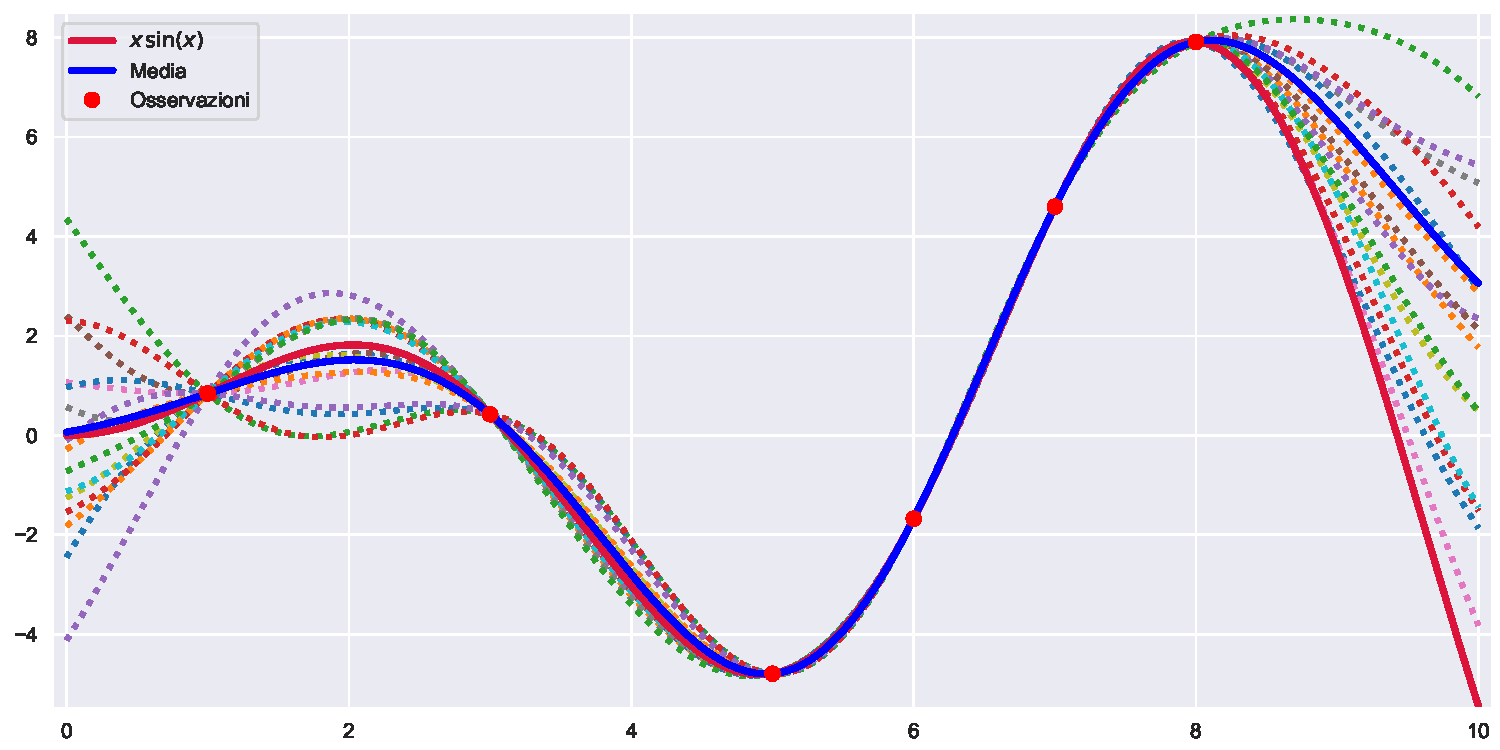
\includegraphics[width=1\textwidth]{images/Gaussian process/Noise-free - mean&f(x).pdf}
    \caption{Graph of functions with distribution $f\sim \mathcal{GP}(\bm{0},k)$ dove $k(\cdot,\cdot)$ is the squared-exponential kernel; the Gaussian process was conditioned to interpolate six points. Shown in red is the function from which the points to be interpolated were chosen, in blue the mean of the conditioned Gaussian process, as dashed lines some samples of the Gaussian process. Code \ref{interpolation code}.}
    \label{Interpolation}
\end{figure}

The mean of the conditional Gaussian process to interpolate the six points is the most reliable in predicting the function $x\cdot sin(x)$ from which the points to be interpolated were generated. The functions with distribution the conditional Gaussian process all have the property of interpolating the aforementioned points, however, in the rest of the plane they are more easily distanced from the mean, although they tend to stay in its vicinity. In Figure \ref{Interpolation confidence region} information from the a posteriori covariance matrix is exploited to draw the 95\% confidence region, within which most of the samples reside.


\newpage
%%%%%%%%%%%%%%%%%%%%%%%%%
%%%%%%%%% IMMAGINE
%%%%%%%%%%%%%%%%%%%%%%%%
\begin{figure}[h]
    \centering
    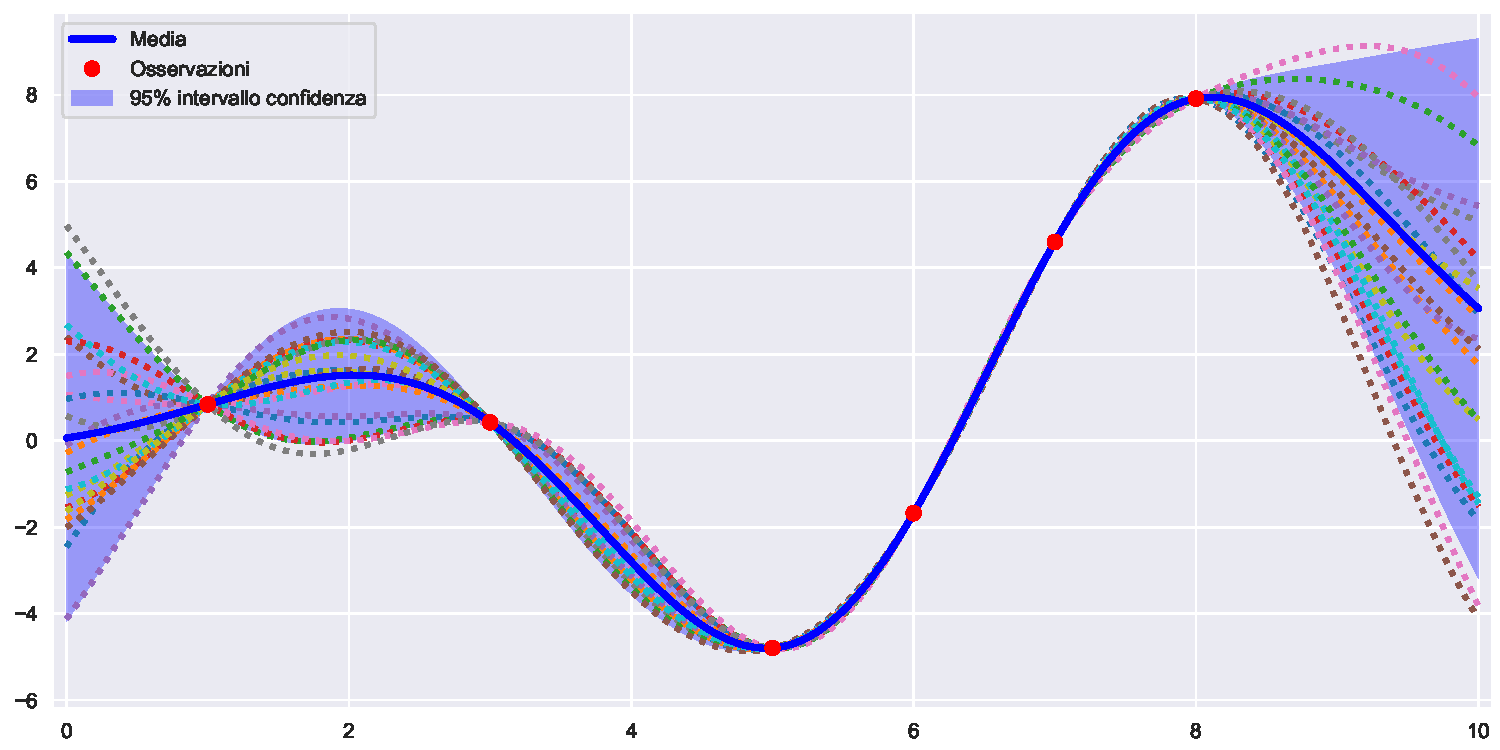
\includegraphics[width=1\textwidth]{images/Gaussian process/Noise-free - mean&samples.pdf}
    \caption{Graph of functions with distribution $f\sim \mathcal{GP}(\bm{0},k)$ where $k(\cdot,\cdot)$ is the squared-exponential kernel; the Gaussian process was conditioned to interpolate six points. Shown in blue is the 95\% confidence region, in blue the mean of the conditional Gaussian process, and as dashed lines some samples. Code \ref{interpolation confidence region code}.}
    \label{Interpolation confidence region}
\end{figure}

As anticipated, within the area given by $\bm{\mu^*}(x_i)\pm 1.96\bm{\Sigma^*}(x_i,x_i)$ (95\% confidence region) reside most of the samples of the a posteriori distribution. The farther one moves away from the interpolated points, the more easily the functions deviate from the mean, tending to move out of the area of uncertainty, as observed, for example, in the area near $x=10$ in Figure \ref{Interpolation confidence region}.



\section{Predictions with noisy observations}\label{noisyPrediction}
This section explains how to exploit the information provided by \textit{training data} to generate a function that incorporates a priori knowledge in the case of observations with noise. \\

\begin{defi}[Noisy training set]
  The \textbf{noisy training set} is the set of \textit{noisy} observations (i.e., with an error component) defined as: $\mathcal{D}=\{(x_n,y_n): n=1,... ,N\}$ where $y_n=f(x_n)+\epsilon$ is the observed value of the function $f$ at the point $x_n$ with a noise component $\epsilon\sim \mathcal{N}(0,\sigma_n^2)$ independent and identically distributed. 
\end{defi}
In this case you have:
\[
\text{Cov}(y_p,y_q)=k(x_p,x_q)+\sigma_n^2 \delta_{pq},
\]
or equivalently:
\[
\text{Cov}(\mathbf{y})=k(X,X)+\sigma_n^2I.
\]

\newpage

A notation analogous to the \ref{regressioneGP} section is used: $X^*=\{x_i^*: i=1,\dots,N^*\}$ is the \textit{test set} whose outputs are to be predicted $\bm{f^*}=\left[f(x^*_1), \dots, f(x^*_{N^*}) \right]$; $\bm{y}=\left[f(x_1)+\epsilon, \dots, f(x_N)+\epsilon \right]$ the outputs of the training set. \\
We proceed as in the case of prediction with noiseless observations:
\[
\begin{pmatrix}
\bm{y}\\
\bm{f^*}
\end{pmatrix}
=
\mathcal{N}\left(
\begin{pmatrix}
\bm{\mu}\\
\bm{\mu_*}
\end{pmatrix},
\begin{pmatrix}
\bm{K}_{X,X}+\sigma_n^2I & \bm{K}_{X,X^*}\\
\bm{K}_{X^*,X} & \bm{K}_{X^*,X^*}
\end{pmatrix}
\right)
\]
It is derived:
\[
\bm{f^*} | X^*, \mathcal{D} \sim \mathcal{N}(\bm{\mu^*}, \bm{\Sigma^*})
\]
where:
\[
\begin{split}
\bm{\mu^*}=m(X^*)+\bm{K}_{X,X^*}^\text{T}(\bm{K}_{X,X}+\sigma_n^2I)^{-1}(\bm{y}-m(X))\\
\bm{\Sigma^*}=\bm{K}_{X^*,X^*}-\bm{K}_{X,X^*}^\text{T}(\bm{K}_{X,X}+\sigma_n^2I)^{-1}\bm{K}_{X,X^*}
\end{split}
\]


A graphic example of how a Gaussian process interprets information given by observations with noise to predict a function is shown in Figure \ref{Noisy}.
As might be expected, since the observations in this case are with noise, the Gaussian process needs more observations in order to predict the trend of the function. Since interpolation does not occur, the Gaussian process predicts the function with less accuracy.
%%%%%%%%%%%%%%%%%%%%%%%%%
%%%%%%%%% IMMAGINE
%%%%%%%%%%%%%%%%%%%%%%%%
\begin{figure}[h]
    \centering
    \includegraphics[width=1\textwidth]{images/Gaussian process/Noise - mean&f(x).pdf}
    \caption{Graph of functions with distribution $f\sim \mathcal{GP}(\bm{0},k)$ where $k(\cdot,\cdot)$ is the squared-exponential kernel; the Gaussian process was conditioned to predict a function from its noisy observations. Shown in red is the function to be predicted, in red the observed points of the function with bars representing the noise, in blue the average of the conditioned Gaussian process, as dashed lines some samples of the Gaussian process. Code \ref{Noise code}.}
    \label{Noisy}
\end{figure}

\newpage

Again, the mean of the conditional Gaussian process represents the function that best predicts $x\cdot sin(x)$. Because the observations have error, there is no interpolation of the points although, it tends to be the case that the mean and samples of the Gaussian process touch at least the error bars of each point.
More points of the noise-free case were taken into account since with fewer points such an "accurate" result would not have been obtained (however, with a different behavior from that with noise-free observations).

If in the noiseless case the samples tended to stay near the mean in the vicinity of each interpolated point, here the closeness to the mean depends on both the points and their error: near points with lower noise (i.e., shorter bars) the functions tend to move closer to the mean. Conversely, near features with a large error (longer bars) the features tend to move away from the mean more easily.

Again, the 95\% confidence region can be drawn. The confidence region has amplitude proportional to the length of the bars of the observations; consequently, the confidence region has markedly different behavior from the noise-free case.

%%%%%%%%%%%%%%%%%%%%%%%%%
%%%%%%%%% IMMAGINE
%%%%%%%%%%%%%%%%%%%%%%%%
\begin{figure}[h]
    \centering
    \includegraphics[width=1\textwidth]{images/Gaussian process/Noise - mean&samples.pdf}
    \caption{Graph of functions with distribution $f\sim \mathcal{GP}(\bm{0},k)$ where $k(\cdot,\cdot)$ is the squared-exponential kernel; the Gaussian process was conditioned to predict a function from its noisy observations. Shown in blue is the 95\% confidence region, in red with error bars the observations, in blue the mean of the conditioned Gaussian process, and as dashed lines some samples. Code \ref{Noise confidence region code}.}
    \label{Noisy confidence region}
\end{figure}
\chapter{Machine learning}\label{machineLearning}

The chapter briefly explains the theory of \textbf{supervised learning} focusing in the context of regression with Gaussian processes. It theoretically introduces the statistical model that will be used to produce results related to the Windkessel model seen in the chapter \ref{windkessel}.\\
The sources used for the drafting of the chapter are: \cite{murphy_probabilistic_2022}, \cite{wiki:datasets}, \cite{wiki:overfitting}, \cite{pytorch:R2score}, \cite{wang_intuitive_2022}, \cite{noauthor_tutorial_nodate}, \cite{murphy_machine_2012}, \cite{gelman_bayesian_1995}, \cite{wiki:gradientDescend}, \cite{ruder_2022}, \cite{kingma_adam_2017}, \cite{JMLR:v12:duchi11a}, \cite{bottou2012stochastic}.


\begin{textblock*}{0.64\textwidth}(3.5cm+0.36\textwidth,18.5cm)
\epigraph{Il sole è sorto e tramontato per miliardi di anni. Il sole è tramontato anche stanotte. Con un'elevata probabilità, il sole domani sorgerà. Ma questo numero è molto più grande per colui che, vedendo nella totalità dei fenomeni il principio che regola i giorni e le stagioni, si rende conto che nulla al momento attuale può arrestarne il corso.}{Pierre Simon Laplace}
\end{textblock*}

\newpage

\section{Introduction to machine learning}
Machine learning is a branch of artificial intelligence, a discipline that studies the theoretical foundations and techniques that enable the design of systems capable of providing computers with performances that would seem to be the exclusive domain of human intelligence.\\
Of this vast branch, the work is only interested in regression problems, as opposed to classification problems.

In more practical terms, the main purpose of machine learning is the study and construction of algorithms that can learn to make predictions about data. Such algorithms work by relying on decisions guided by the dataset through the construction of a mathematical model.\\
A specific type of learning is used in this work, which is the \textit{supervised} learning.

\begin{defi}[Supervised learning]
    \textbf{Supervised learning} is a machine learning technique that aims to instruct a computer system to make predictions based on a series of examples consisting of input and output pairs.
\end{defi}

\section{Dataset}\label{dataset}

Per ottimizzare la costruzione di algoritmi predittivi, i dati di input vengono divisi in più set di dati con ruoli diversi. Tipicamente viene usata una specifica partizione dei dati in tre dataset: \textbf{training}, \textbf{validation} e \textbf{test set}.


\begin{defi}[Training set]
Il \textbf{training set} è un insieme di esempi utilizzati durante il processo di apprendimento per determinare (o imparare) le combinazioni ottimali di parametri.
\end{defi}

In pratica, è sui dati del training set che viene eseguito il metodo di ottimizzazione scelto, aggiornando quindi i valori dei parametri o degli iperparametri.

\begin{defi}[Validation set]
Il \textbf{validation set} è un set indipendente di dati usato per valutare il modello addestrato sul training set.
\end{defi}
La valutazione (o \textit{validazione}) del modello sul validation set porta a decidere quali siano i migliori valori per i parametri (o iperparametri) in base alla performance sul validation set, appunto. Nel caso dell'elaborato viene usato un early-stopper, che sceglie come miglior modello quello con minore errore subito prima che si verifichi overfitting.

\begin{defi}[Test set]
Un \textbf{test set} è un set indipendente di dati dal training set  usato solo per valutare le prestazioni del modello.
\end{defi}

\newpage

Cioè il test set viene usato per valutare su un terzo set di dati indipendente il modello scelto in base alla performance sul validation set. Si ottengono così caratteristiche di prestazione come la precisione, la sensibilità, la specificità... Questo dataset è importante perché permette di valutare la performance del modello su un terzo insieme di dati indipendente dai precedenti evitando il rischio di overfitting: se un modello addestrato sul training test si adatta anche al test set, si è verificato un overfitting minimo.

È stato più volte citato il problema dell'\textbf{overfitting}, viene quindi riportata la definizione.

\begin{defi}[Overfitting]
L'\textbf{overfitting} è la generazione di un modello (o un'analisi) che corrisponde troppo strettamente a un particolare insieme di dati e può quindi non riuscire a prevedere osservazioni future in modo affidabile.
\end{defi}

L'overfitting può verificarsi per esempio includendo troppi parametri regolabili o usando un approccio troppo complicato, come mostrato in figura \ref{overfittigComplex}. Chiaramente, quando si confrontano diversi tipi di modelli la complessità deve tenere conto dell'influenza di ogni parametro sull'output\footnote{Si noti che si può incorrere nel problema opposto usando un approccio troppo semplice: l'underfitting. Ad esempio cercando di approssimare con una regressione lineare un campione con un andamento parabolico.}.

\begin{figure}[htbp]
    \centering
    \includegraphics[width=0.6\textwidth]{images/Machine learning/Overfitted_Data.png}
    \caption{Esempio di overfitting. I dati (approssimativamente lineari) sono approssimati da una funzione lineare e da una polinomiale. Anche se la funzione polinomiale fornisce un adattamento quasi perfetto, ci si può aspettare che la funzione lineare generalizzi meglio i dati. \cite{wiki:overfitting}}
    \label{overfittigComplex}
\end{figure}

\newpage

L'overfitting è particolarmente probabile nei casi in cui l'apprendimento è stato eseguito troppo a lungo o in cui ci sono pochi dati per l'apprendimento, facendo sì che il modello si adatti a caratteristiche casuali molto specifiche dei dati di formazione che non hanno alcuna relazione causale con l'output. In questo caso di overfitting, la performance sul training set continua ad aumentare mentre la performance sul validation set peggiora, come mostrato in figura \ref{overfittingError}.



\begin{figure}[htbp]
    \centering
    \includegraphics[width=0.6\textwidth]{images/Machine learning/Overfitting error.png}
    \caption{Overfitting nell'apprendimento supervisionato. Il training error (errore sul training set) è mostrato in blu, il validation error (errore su validation set) in rosso, entrambi in funzione del numero di cicli di training. \cite{wiki:overfitting}}
    \label{overfittingError}
\end{figure}


\subsection{Loss function}
Finora è stato delineato il problema che interessa l'elaborato: cercare una funzione $f$ per predire l'output $Y$ a partire dai valori dell'input $X$. Per farlo è necessaria una funzione di perdita, in inglese \textit{loss function}, $L(Y, f (X))$ per penalizzare gli errori di previsione.

\begin{defi}[Loss function]
Una \textbf{loss function} è una funzione in forma $\mathcal{L}(y_{\text{true}},y_{ \text{guess}})$ che definisce la perdita subita (o l'errore commesso) predicendo il valore $y_\text{guess}$ quando il valore vero è $y_{\text{true}}$,  fornendo quindi una valutazione delle capacità predittive del modello.
\end{defi}

Sarà questa la funzione da minimizzare con un algoritmo di ottimizzazione per l'adattamento degli iperparametri del processo gaussiano. Evidentemente la scelta della loss function dipende dal contesto.

%\section{Mean squared error}
%Per gli scopi dell'elaborato, si farà uso del \textit{mean squared error}.

%\begin{defi}[Mean squared error]
%Il \textbf{mean squared error} (o \textit{MSE}) è una \textit{loss function} definita come:
%\[
%\frac{1}{n}\sum^{n}_{i=1}(Y_i-f(X_i))^2,
%\]
%dove su $n$ dati raccolti, $Y_i$ sono gli output reali, $f(X_i)$ sono gli output predetti a partire da $X_i$.
%Poiché deriva dal quadrato della distanza euclidea, è sempre un valore positivo che diminuisce man mano che l'errore si avvicina a zero.
%\end{defi}
%Verrà usato non come loss function, ma per monitorare l'andamento del training.


%\section{Coefficiente di determinazione}
%Il coefficiente di determinazione fornisce una misura della bontà di adattamento di un modello, cioè quanto le previsioni di regressione approssimano i punti dei dati reali. Varia tra 0 e 1\footnote{Si possono apportare modifiche al coefficiente per fargli assumere anche altri valori, ma non vengono applicate nell'elaborato}, un $R^2$ di 1 indica che le previsioni di regressione si adattano perfettamente ai dati.

%Poichè il coefficiente di determinazione varia in un intervallo unitario, può essere più (intuitivamente) informativo di altre misure di errore (come il mean absolute error o il mean squared error) poiché tendono ad assumere valori su intervalli arbitrari oppure ad esprimere una percentuale.

%\begin{defi}[Coefficiente di determinazione]
%Date $y_i$ le osservazioni, $\overline{y}$ la media delle osservazioni, $\hat{y}_i$ i dati predetti dal modello:
%\[
%R^2 = 1-\frac{\sum_{i=1}^{n}(y_i-\hat{y}_i)}{\sum_{%i=1}^{n}(y_i-\overline{y})}
%\]
%\end{defi}
%Si noti che questo coefficiente non indica se:
%\begin{itemize}
%    \item una variabile sia statisticamente %significativa;
%    \item è stata usata la regressione corretta;
%    \item è stato scelto l'insieme più appropriato %di variabili indipendenti;
%    \item ci sono abbastanza dati per trarre una %conclusione solida.
%\end{itemize}

%Si noti inoltre che $R^2$ è una versione riscalata del mean squared error più facile da interpretare in quanto non dipende dalla scala dei dati.

\newpage
\section{Parametric and non-parametric models}
There is an important distinction to be made about statistical models: parametric and non-parametric models. The type of model, in fact, greatly modifies the theoretical approach to be used and thus the application results. 


\subsection{Parametric models}
Parametric models assume that the distribution of data can be modelled in terms of a finite set of parameters.\\
A classic example is regression in which, given observations, an attempt is made to estimate a possible functional relationship existing between the dependent variable and the independent variables. If we assume a linear regression model, where the relationship is expressed by the function $f(x) = \theta_1 + \theta_2x$ where $x$ is the input data, we need to find the values of the parameters $\theta_1$ and $\theta_2$ to define $f$. In many cases, the assumption of the linear model is not sufficient, and a polynomial model (with more parameters) is needed: $f(x) = \theta_1+\theta_2x+\theta_3x^2$.\\
Thus given a dataset $D$ with $n$ observed points, after the process of \textit{training} we assume that all information about the functional relationship has been captured by the parameters $\theta_i$.  When running regressions using parametric models, the complexity and flexibility of the models is limited by the number of parameters. 

\subsection{Non-parametric models}
Contrary to what one might think, a \textbf{non-parametric model} is not a model without parameters. \\
Intuitively, if the number of parameters of a model increases with the size of the observed dataset, it is a non-parametric model. Theoretically, this allows the model to have infinite parameters and thus not depend on a rigid function structure $f$, increasing its flexibility.\\
Of interest in the paper is regression using Gaussian processes, which follows a non-parametric Bayesian approach (seen in \ref{regressioneGP}). It is capable of \textit{learning} a wide variety of input-output relationships using a theoretically infinite number of parameters and letting the data determine the level of complexity through the means of Bayesian inference.

See \ref{gerarchica} for a clarification of the difference between parameters and hyperparameters in regression using Gaussian processes.

\newpage

\subsection{Hierarchical structure}\label{gerarchica}
It is common to use a hierarchical structure of parameters and hyperparameters in regression models.

The parameters reside at the lowest level. For example, in the case of linear regression, the parameters are the $\theta_i$, or in the case of a neural network model the weights associated with the neurons.\\
At the second level are the \textit{iperparameters} that control the distribution of parameters at the lower level and thus whose value is used to control the learning process.\\

In the case of Gaussian processes, since they are a non-parametric model, it is not obvious what the parameters of the model are. One can take the values of the (noise-free) function evaluated on the observed data as parameters. Then let $X=\{(x_i,y_i): i\in I\}$ be the set of observed data, the elements $y_i$ can be considered the parameters of the model. Obviously, the larger $X$, the more parameters there are. In practical terms, it was seen in \ref{regressioneGP} how the observed data correspond to the information about the shape of the function, thus how the accuracy depends on the number of observed data.

It is also possible to give a different interpretation of the model parameters using a different theoretical interpretation (\textit{weight-space view}), which has not been introduced in the paper.\footnote{Further: \cite{rasmussen_gaussian_2006}}\\

The hyperparameters, on the other hand, are the parameters of the mean function and the kernel function. Pragmatically, to do regression, it is necessary to work on the estimation of the hyperparameters.


\newpage


\section{Optimisation of hyperparameters}

\subsection{Bayesian inference}
Bayesian inference is a method of statistical inference in which Bayes' theorem is used to update the probability of a hypothesis as more information becomes available. 

The Bayesian process of data analysis can be idealised by dividing it into the following three stages:
\begin{enumerate}
    \item Creation of a complete probability model\\
    The model consists of a joint probability distribution for all quantities related to the problem and must be consistent with the knowledge of the underlying scientific problem.
    \item Conditioning of observed data\\ The appropriate a posteriori distribution, i.e. the probability distribution of the unobserved quantities conditioned on the observed data, is calculated and interpreted.
    \item Evaluation of model fit\\
    It is assessed how well the model fits the data and whether the substantive conclusions are reasonable. At this stage, it is possible to modify or expand the model and repeat the three steps.
\end{enumerate}
The Bayesian approach can be interpreted as a formalisation of the scientific method, in which an attempt is made to update scientific knowledge through experiments and observations.\\
Moreover, this statistical approach is flexible enough to be used in complex problems, even those with many parameters.\\

In the area of Gaussian processes, the use of Bayesian inference in the optimisation of hyperparameters is studied.

\newpage

\subsection{Bayes' Theorem}
\begin{teo}[Bayes' Theorem]
    Let $A, B$ be events, let $\probP(B)\neq 0$, then:
\[
\probP(A|B) = \frac{\probP(B|A)\probP(A)}{\probP(B)}.
\]
\end{teo}
\begin{proof}
    From the definition of conditional probability we have: $\probP(A\cap B) = \probP(A|B)\probP(B)$, from which it follows $\probP(A|B)=\frac{\probP(A\cap B)}{\probP(B)}$ if $\probP(B)\neq 0$; similarly: $\probP(B|A)=\frac{\probP(A\cap B)}{\probP(A)}$ if $\probP(A)\neq 0$. Substituting $\probP(A\cap B)$ into the expression of $\probP(A|B)$ concludes.
\end{proof}

\vspace{0.5cm}

In the Bayesian context, the purpose of analysing a model is to draw statistical conclusions about a parameter $\theta$ (or similarly about a vector of parameters\footnote{For the moment, the case of parameters is considered, but what is said immediately extends to the case of hyperparameters, as seen in \ref{evidenzaBayesiana}}) or about unobserved data; these conclusions are formulated in terms of probabilities conditional on the observed value of $y$. 
In order to make probability statements on $\theta$ observed $y$ data, it is necessary to start with a model that provides a joint probability distribution for $\theta$ and $y$, which can be factored into two components: $\probP(\theta)$, i.e. the a priori distribution describing the knowledge about the distribution of $\theta$ before observing the data, and $\probP(y|\theta)$, i.e. the data (or sample) distribution:
\[
\probP(\theta, y)=\probP(\theta)\probP(y|\theta).
\]

Applying Bayes' theorem we obtain the \textit{a posteriori distribution}:
\[
\probP(\theta | y)=\frac{\probP(\theta)\probP(y|\theta)}{\probP(y)},
\]
in which the denominator can be rewritten, by the absolute probability theorem (\textit{law of total probability}), as:
\[
\probP(y)=\begin{cases}\sum_\theta \probP(\theta)\probP(y| \theta)\\\int\probP(\theta)\probP(y| \theta)d\theta \end{cases} \text{ in base a }\theta.
\]
Since $\probP(y)$ does not depend on $\theta$ and fixing $y$ it is possible to rewrite the a posteriori distribution as:

\[
\probP(\theta | y)\propto \probP(\theta)\probP(y|\theta),
\]
where, having fixed $y$, $\probP(y|\theta)$ is a function of $\theta$.

\newpage

\subsection{Bayesian evidence}\label{evidenzaBayesiana}
In the context of statistical models, the reinterpretation of Bayes' theorem (and what was said in the previous section) is:
\[
\probP(\theta | X, \alpha) = \frac{\probP(X|\theta, \alpha)\probP(\theta | \alpha)}{\probP(X|\alpha)}\propto \probP(\theta | \alpha) \probP(X|\theta, \alpha),
\]
where: $\theta$ is the vector of parameters, $\alpha$ the vector of hyperparameters, $X$ the sample of observed data. In this case the a priori distribution is $\probP(\theta|\alpha)$\footnote{ Note that it is conditional on the value of the hyperparameters. This is due to the definition of the hyperparameters, which control the distribution of the parameters, as mentioned in \ref{gerarchica}. }, the distribution of the parameters before observing the data $X$; $\probP(X|\theta)$, the sample distribution which is the distribution of the observed data conditional on the value of the parameters; and $\probP(X|\alpha)$, the \textbf{evidence} (also called \textit{marginal likelihood}) which is the distribution of the data conditional on the hyperparameters. The latter can be rewritten as
\[
\probP(X|\alpha) = \int \probP(X|\theta)\probP(\theta | \alpha)d\theta,
\]
i.e. as the distribution of marginalised data on the parameters.

In addition to being the normalisation term in Bayes' theorem, another possible way of interpreting marginal likelihood is to consider it the probability of having generated the (observed) dataset $X$ given the hyperparameters $\alpha$.

Using Bayes' theorem again, we obtain:
\[
\probP(\alpha |X) = \frac{\probP(X|\alpha)\probP(\alpha)}{\probP(X)}\propto \probP(X|\alpha) \probP(\alpha),
\]
i.e. the a posteriori distribution (representing the distribution of the observed hyperparameters of the $X$ data) is proportional to the marginal likelihood. Since in the case considered by the paper, i.e. Gaussian processes, one of the objectives is to find the distribution of the hyperparameters (i.e. the form of the covariance function, in other words $\probP(\alpha|X)$)), the approach adopted is to maximise the marginal likelihood, taking advantage of the dependence highlighted in the previous formula. This approach is called the \textbf{evidence approach}.

\newpage

\subsection{Alternatives to Bayesian evidence}
The choice of approach for estimating the value of parameters or hyper-parameters depends very much on the situation. For example:
\begin{itemize}
    \item Maximising the \textit{likelihood}:
    one maximises $L(\alpha, \theta | X)$ (the likelihood function), thus finding values of $\alpha$ and $\theta$ that maximise it;
    \item Partial maximisation of \textit{likelihood}:
    Given the case in which $L(\alpha, \theta |X)=L_1(\alpha | X)L_2(\theta|X)$, only the factor of interest is maximised, in the present case $L_1(\alpha | X)$ is maximised;
    \item Maximising the \textit{marginal likelihood}:
    marginalises on $\theta$, then maximises $\probP(X|\alpha)$ which depends only on $\alpha$.
\end{itemize}
The paper applies the last case since the necessary calculations are all analytically solvable. In other situations, this approach requires a numerical approximation which may lead to stability problems, which is why it is not always an approach used.




\subsection{In Gaussian processes}\label{neiProcessiGaussiani}
The approach that Gaussian processes follow is to define a \textit{distribution over functions}, update it from observed data and use it to make predictions on new inputs. \\
Consider what was done in the section \ref{noisyPrediction}: an a priori distribution was defined on the functions, which was then converted into an a posteriori distribution by updating the information thanks to the observed data. Unlike the \textit{noise-free} case, however, one does not obtain a function that perfectly interpolates the data. In this case, it is therefore necessary to choose appropriate hyperparameters in order to optimise the form of the function: this estimation is done by means of an evidence approach, taking advantage of the fact that the expressions of the integrals are all analytically solvable.\\


In this case, the marginal likelihood is:
\[
\probP(\bf{y}|\bf{\alpha}) = \int \probP(\bf{y}| \mathbf{f},\bf{\alpha})\probP(\mathbf{f}|\bf{\alpha}) d\mathbf{f},
\]

where $\bf{\alpha}$ are the hyperparameters, $\mathbf{f}$ are observed data without error (they are the parameters), $\bf{y}$ are the observed data.\\
Note that $\probP(\mathbf{f}|\bf{\alpha})$ is the a priori distribution of the error-free function and is a multivariate Gaussian distribution since $\mathbf{f}|\alpha\sim \mathcal{N}(m, K)$ with $K$ the Gram matrix of the covariance function and $m$ the evaluation of the mean function on the input vector. Furthermore, from the definition of $\mathbf{y}$ we have $\mathbf{y}|\mathbf{f}\sim \mathcal{N}(\mathbf{f}, \sigma_n^2I)$, where $\epsilon\sim \mathcal{N}(0,\sigma_n^2)$.

\newpage

The calculations reported in \cite{rasmussen_gaussian_2006} conclude:
\[
L=\text{log}(\probP(\mathbf{y}|\alpha))=-\frac{1}{2}\text{log}(|K+\sigma_n^2I|)-\frac{1}{2}(\mathbf{y}-m)^{\text{T}}(K+\sigma_n^2I)^{-1}(\mathbf{y}-m)-\frac{n}{2}\text{log}(2\pi)
\]

The same result can be obtained by avoiding analytical accounts by noting: $\mathbf{y}\sim \mathcal{N}(m, K+\sigma_n^2I)$. At this point, it is easy to calculate the partial derivatives with respect to the hyperparameters of the covariance function and the mean function. This is of fundamental importance for numerical optimisation methods.

Note that marginal likelihood maximisation is preferable to likelihood maximisation (or other likelihood methods) because with other forms of likelihood overfitting can be achieved (see \ref{dataset} for the definition of overfitting). In contrast, marginal likelihood does not perform \textit{fitting} of function values, but rather integrates (marginalises) them, i.e. technically it cannot do overfitting because no \textit{fit} occurs. \\

For further considerations, account details and insights on how to optimise numerical calculations, see \cite{rasmussen_gaussian_2006}.




\section{Optimisation method}
Optimisation is the branch of mathematics that studies theory and methods for finding the maximum and minimum points of a function. This section aims to retrace the main theoretical steps that led to the construction of the optimisation method later used in marginal likelihood maximisation: Adam.

\subsection{Form of the function to be optimised}\label{costfunction}
In order to understand the difference between the optimisation methods shown, it is important to understand the form of the function to be optimised.
In supervised learning, we have a dataset of observations that we want to learn from. To do this, in short, we define a function that represents the error that our model makes on the dataset of observed values\footnote{See the section \ref{dataset}, where we explain how to divide a dataset into subsets with different roles.}: the goal is to minimise this function, and to do this, it is necessary, using an appropriate algorithm, to change the values of the parameters (in the case under consideration, a non-parametric model, the hyperparameters are changed).

\newpage

Since the observed dataset will potentially contain a lot of data, it is necessary to take into account the error committed by evaluating it in each observed dataset. Generally, the error function has a form:
\[
Q(w)=\sum_{i=1}^{n}Q_i(w),
\]
where each addend tends to depend on a single datum in the input dataset. An example is:
\[
f(m,b)=\sum_{i=1}^{N}(y_i-(mx_i+b))^2,
\]
i.e. the method of least squares in linear regression.\\
Note that in the present case, the function to be optimised, the marginal likelihood, is a sum in which the $i$-th addend does not depend only on the $i$-th observed data.


\subsection{Learning rate}
The iterative optimisation methods have a similar form: given $\theta_0$ initial point, each iteration updates the point as:
\[
\theta_{t+1}=\theta_t+\eta_td_t,
\]
where $d_t$ represents a direction and is defined according to the method, $\eta_t$ is the step length (\textit{step size}) or \textit{learning rate} and indicates by how much one moves in the direction $d_t$. The learning rate can be constant or can be updated every iteration.


\newpage

\subsection{Gradient method \cite{ruder_2022}}
The \textbf{gradient method} exploits the fact that the gradient is the direction of maximum growth of the function. It has a form:
\begin{align*}
    &\text{Given an initial value }\omega_0, \eta_0\\
    &\text{To be repeated until an approximation of the minimum is found:}\\
    &\quad \omega_{k+1}=\omega_k - \eta_k\cdot \nabla Q(\omega_k).
\end{align*}
By "\textit{Repeat until an approximation of the minimum is found}" is meant that the method is repeated until an output condition is met that incorporates the precision required of the approximation.\\
Since, as seen in \ref{costfunction}, it is necessary to evaluate the gradient on each element of the dataset, it can be an onerous method, especially in terms of memory.\\
The learning rate $\eta_k$ can be constant for each $k$ or it can be changed at each iteration. In both cases, it plays an important role as it may lead, if too small, to too slow convergence or, if too large, to divergence. In the case of a learning rate updated at each iteration, we generally decrease it as we approach the minimum; for example see figure \ref{gradientDescentImage}.

\begin{figure}[h]
    \centering
    \includegraphics[width=0.6\textwidth]{images/Training (teoria)/Gradient descend.png}
    \caption{Illustration of the gradient method on level sets, the learning rate is updated at each iteration.\cite{wiki:gradientDescend}}
    \label{gradientDescentImage}
\end{figure}



\subsection{Stochastic gradient descent \cite{bottou2012stochastic}}
The method of \textbf{stochastic gradient descent}, unlike the gradient method, performs an update for each $Q_i$\footnote{In the case where the $Q$ is written as a sum of terms that each depend only on one element of the dataset, it implies that the method performs an update for each element of the dataset}. It has the form:
\begin{align*}
    &\text{Given an initial value }\omega_0, \eta_0\\
    &\text{To be repeated until an approximation of the minimum is found:}\\
    &\quad\text{Mixing the dataset}\\
    &\quad\text{For }i=1,...,n:\\
    &\quad\quad\omega_{k+1}=\omega_k -\eta_k\cdot \nabla Q_i(\omega_k)
\end{align*}
Since we only have to calculate the gradient for one addend of $Q$ at a time, it is a much faster method, although these frequent updates cause a high fluctuation of the objective function, as can be seen from the figure \ref{MomentumMethod}.\\
Although fluctuation may seem a disadvantage of the method, it is precisely this that allows it to avoid local minima and tend towards better approximations. The gradient method seen above, on the other hand, converges to the minimum of the basin in which the initial data was chosen.\\
On the other hand, fluctuation complicates convergence to the exact minimum due to the frequent changes the function undergoes. However, it has been shown that when slowly decreasing the learning rate, the method shows the same convergence behaviour as the gradient method. 


\newpage
\subsection{Method of moments \cite{ruder_2022}}
The stochastic gradient method has difficulty traversing \textit{burrows}, i.e. areas where the surface curves more steeply in one dimension than another. In these scenarios, the method oscillates along the slopes of the gully, while it hesitantly progresses along the bottom towards the minimum, as shown in the figure \ref{MomentumMethod}.\\
The \textbf{momentum method} is a method that helps accelerate the stochastic gradient method in the desired direction and dampen oscillations, as seen in the figure \ref{MomentumMethod}. It has the form:

\begin{align*}
    &\text{Given an initial value }\omega_0, \eta_0, v_0=0\\
    &\text{To be repeated until an approximation of the minimum is found:}\\
    &\quad\text{Mix the dataset}\\
    &\quad\text{For }i=1,...,n:\\
    & \quad\quad v_t=\gamma v_{t-1}+\eta_k\cdot \nabla Q_i(\omega_k)\\
    &\quad\quad\omega_{k+1}=\omega_k - v_t
\end{align*}
The $\gamma$ term is called \textit{momentum} (or \textit{quantity of motion}) and is usually set to 0.9.\\
Basically what happens is analogous to when you push a ball down a hill: the ball accumulates momentum
as it rolls downhill getting faster and faster (until it reaches its terminal velocity, if there is
air resistance, i.e. $\gamma<1$). 
The same thing happens with parameter updates: in the vector, the "momentum" term favours the dimensions in which the gradient points in the same direction and disfavours the others. As a result, faster convergence and reduced oscillation is achieved, reducing the problems of the stochastic gradient method, as shown in figure \ref{MomentumMethod}.

\begin{figure}[h]
\centering
\begin{subfigure}{.5\textwidth}
  \centering
  \includegraphics[width=\linewidth]{images/Training (teoria)/SGD Momentum a.PNG}
  \caption{Without momentum.}
\end{subfigure}%
\begin{subfigure}{.5\textwidth}
  \centering
  \includegraphics[width=\linewidth]{images/Training (teoria)/SGD Momentum b.PNG}
  \caption{With momentum.}
\end{subfigure}
\caption{Method of moments applied to the stochastic gradient method. \cite{ruder_2022}}
\label{MomentumMethod}
\end{figure}

\newpage
\subsection{AdaGrad \cite{JMLR:v12:duchi11a}}
The \textbf{AdaGrad} method (short for \textit{Adaptive Gradient algorithm}) is an optimisation algorithm based on the stochastic gradient method that uses an independent learning rate for each $\omega_i$. For $\omega_i$ terms that have a higher gradient or frequent updates, the method imposes a lower learning rate so as not to exceed the minimum. Conversely, those with a low gradient or infrequent updates will have a higher learning rate, so as to be trained quickly.\\



Adagrad improves the robustness of the stochastic gradient method and converges more quickly, especially when the data distribution is sparse; it has demonstrated excellent results in the training of large-scale neural networks (e.g. Google).

\begin{align*}
    &\text{Given an initial value }\omega_0, \eta\\
    &\text{To be repeated until an approximation of the minimum is found:}\\
    &\quad\text{Mix the dataset}\\
    &\quad\text{For }i=1,...,n:\\
    &\quad\quad \text{For each component $j$ of $\omega$:}\\
    &\quad\quad\quad g_{k,j}=(\nabla Q_i(\omega_k))_j\\
    &\quad\quad\quad\omega_{k+1,j}=\omega_{k,j} - \frac{\eta}{\sqrt{G_{k,j}}+\epsilon}g_{k,j}
\end{align*}
Where $G_{k,j}=\sum_{t=1}^{k}g_{t,j}^2$ and $\epsilon$ a small term to avoid division by zero (usually $10^{-8}$).\\
Since it adapts the learning rate, one of the main advantages of the method is that it eliminates the need to manually adjust $\eta_k$: generally $\eta=0.01$ is set.\\
The weak point of Adagrad is the accumulation of squared gradients in the denominator: as each added term is positive, the accumulated sum continues to grow during training. This causes the learning rate to decrease and tend to become infinitesimally small, at which point the algorithm is no longer able to acquire further knowledge.


\newpage
\subsection{Adam \cite{kingma_adam_2017}}\label{adam}
The \textbf{Adam} method (short for \textit{Adaptive Moment Estimation}) is, like the previous one, an adaptive learning rate method for each parameter. It derives from other methods (AdaDelta, RMSprop) that attempt to reduce the monotonically decreasing learning rate of the AdaGrad method. In fact: instead of accumulating all past gradients squared, the sum of the gradients is recursively defined as a decreasing average of all past quadratic gradients, which thus depends on the previous average and the current gradient, and is called $v_k$. Furthermore, Adam's method predicts the same decreasing average of past gradients, called $m_k$.


\begin{align*}
    &\text{Given an initial value }\omega_0, \eta, m_0=0, v_0=0\\
    &\text{To be repeated until an approximation of the minimum is found:}\\
    &\quad\text{Randomly shuffles the dataset}\\
    &\quad\text{For }i=1,...,n:\\
    &\quad\quad \text{For each $j$ component of $\omega$:}\\
    &\quad\quad\quad g_{k,j}=(\nabla Q_i(\omega_k))_j\\
    &\quad\quad\quad m_k=\beta_1m_{k-1}+(1-\beta_1)g_{k,j}\\
    &\quad\quad\quad v_k=\beta_2v_{k-1}+(1-\beta_2)g^2_{k,j}\\
    &\quad\quad\quad \hat{m}_k = \frac{m_k}{1-\beta_1^k}\\
    &\quad\quad\quad \hat{v}_k = \frac{v_k}{1-\beta_2^k}\\
    &\quad\quad\quad\omega_{k+1,j}=\omega_{k,j} - \frac{\eta}{\sqrt{\hat{v_k}}+\epsilon}\hat{m_k}
\end{align*}
The terms $m_k$ and $v_k$, the decreasing averages of the gradients and the square gradients, are estimates of the first moment and the second moment of the gradients, as defined in the method of moments. Since $m_k$ and $v_k$ are biased towards values close to zero, corrected $\hat{m}_k$ and $\hat{v}_k$ estimators are used. We generally impose values $\beta_1=0.9$ and $\beta_2=0.999$.

\newpage
Figure \ref{comparison} compares a number of methods in cost function minimisation in a neural network. It can be seen that Adam's method is much more efficient than the other methods introduced in the paper.
\begin{figure}[h]
    \centering
    \includegraphics[width=0.75\textwidth]{images/Machine learning/Comparison.PNG}
    \caption{Comparison of methods for minimising a cost function in a neural network. \cite{kingma_adam_2017}}
    \label{comparison}
\end{figure}
\chapter{Windkessel model}\label{windkessel}
This chapter introduces some concepts of physiology necessary for understanding the \textbf{Windkessel model}, later introduced. The chapter is not intended to be complete with the theory behind the model, but it is intended to introduce the idea on which it is based: the \textbf{Windkessel effect}.\\
The chapter makes use of a jupyter notebook used in the course \textit{Introduction to Python for Scientific Computing} taught by Professor Lucas Omar Müller in the academic year 2021/2022.\\
The sources used in writing the chapter are: \cite{AaronsonPhilipI.PhilipIrving2020Tcsa}, \cite{wiki:Vascularresistance}, \cite{wiki:Compliance}, \cite{wiki:WindkesselEffect},
\cite{wiki:cicloCardiaco},
\cite{wiki:DiagrammaWiggers},
\cite{westerhof_arterial_2008}, \cite{ghitti_toro_müller_2022}. \\



\begin{textblock*}{0.64\textwidth}(3.5cm+0.36\textwidth,18.5cm)
\epigraph{Medicine is a science of uncertainty and an art of probability.}{William Osler}
\end{textblock*}




\newpage

\section{Introduction}
From \cite{westerhof_arterial_2008} we consider data from a patient in whom aortic flow $Q_{text{in}}$ and systemic pressure $P$ were measured.

Viewing the graph of the two values yields what is shown in figure \ref{figDatiReali}.

\begin{figure}[h]
    \centering
    \includegraphics[width=0.7\textwidth]{images/Windkessel/DatiReali.pdf}
    \caption{Systemic pressure and aortic flow measured in a patient. Code \ref{datiReali}.}
    \label{figDatiReali}
\end{figure}

A simple model of the cardiovascular system is now considered:
\[
P=Q_{\text{in}}R,
\]
Where $R$ is the total peripheral resistance. This model allows calculation of arterial pressure from the blood flow entering the system and the total peripheral resistance.



From the patient's actual data, it is possible to derive the value of total peripheral resistance $R$, or resistance of the cardiovascular system. Given $T$ the duration of the cardiac cycle, we have:
\[
R = \frac{\frac{1}{T}\int_TP(t)dt}{\frac{1}{T}\int_TQ_{\text{in}}(t)dt}.
\]

\newpage

Having derived $R=1.037 mmHg/mL\cdot s$ (as per the code \ref{resistenzatotale}) knowing $Q_{\text{in}}$, it is now possible to use the model to derive the trend of $P$, as shown in Figure \ref{figModelloSemplic}.


\begin{figure}[h]
    \centering
    \includegraphics[width=0.7\textwidth]{images/Windkessel/modelloSemplice.pdf}
    \caption{Real pressure graph and simple model output. Code \ref{modelloSemplice}.}
    \label{figModelloSemplic}
\end{figure}

As is clear from the figure, in the systole phase the model predicts a very high peak pressure (on the order of five times higher than the actual figure). As will be shown in the rest of the chapter, this is because the model neglects a fundamental aspect of arterial circulation: the Windkessel effect, that is, the storage of energy in the arteries during the systole phase.\\
A model that takes this effect into account and thus provides a much more accurate approximation will be proposed at the end of the chapter.


\newpage




\section{Concepts of physiology}

\subsection{Cardiac cycle}
The cardiac cycle, of which a table summary is given \ref{cicloCardiaco}, will not be analyzed in detail, but the period of systole and diastole are briefly described, useful for understanding the next topics. The image \ref{wiki: cuore} may come in handy, so as to have in mind the anatomy of the human heart necessary for understanding the subsequent concepts.

\begin{figure}[h]
    \centering
    \includegraphics[width=0.7\textwidth]{images/Windkessel/Cuore.png}
    \caption{Anatomy of the human heart \cite{wiki:cicloCardiaco}.}
    \label{wiki: cuore}
\end{figure}

Cardiac diastole is the period in the cardiac cycle when, after contraction, the heart relaxes and expands as it fills with returning blood from the circulatory system. Both atrioventricular valves (tricuspid and mitral) open to facilitate the "unpressurized" flow of blood directly through the atria into both ventricles, where it is collected for the next contraction. \\

Atrial systole is the contraction of cardiac muscle cells in both atria as a result of electrical stimulation and conduction of electrical currents through the atrial chambers. \\
Defined as part of the contraction and ejection sequence, atrial systole actually plays the role of completing diastole, that is, finalizing the filling of both ventricles with blood while they are relaxed and expanded for that purpose. 

\newpage

Atrial systole overlaps with the end of diastole and applies contraction pressure to shift blood volumes to both ventricles; this atrial "kick" concludes diastole immediately before the heart begins contracting again and expelling blood from the ventricles (ventricular systole) to the aorta and arteries.\\

Ventricular systole is the contraction, following electrical stimulation, of the ventricular syncytium of heart muscle cells in the right and left ventricles. \\
Right ventricular contractions provide pulmonary circulation by pulsing oxygen-depleted blood through the pulmonary valve and then through the pulmonary arteries to the lungs. Simultaneously, left ventricular systole contractions provide systemic circulation of oxygen-depleted blood to all body systems by pumping blood through the aortic valve, aorta and all arteries.\\
Two simple diagrams depicting the displacement of oxygenated (red) and non-oxygenated (blue) blood in the systole and diastole phases are shown in Figure \ref{sistoleDiastole}.

\begin{figure}[h]
\centering
\begin{subfigure}{0.5\textwidth}
  \centering
  \includegraphics[width=0.5\linewidth]{images/Windkessel/sistole.png}
  \caption{Systole}
\end{subfigure}%
\begin{subfigure}{0.5\textwidth}
  \centering
  \includegraphics[width=0.5\linewidth]{images/Windkessel/diastole.png}
  \caption{Diastole}
\end{subfigure}
\caption{Diagrams summarizing the systole and diastole of a human heart \cite{wiki:cicloCardiaco}.}
\label{sistoleDiastole}
\end{figure}

\newpage

%%%%%%%%%%%%%%%%%%% TABELLA
\begin{landscape}
%%%%%%%%%%%%%%%%%%%%%%%%%%%%%%%%%%%%%%%%%%%%%%%
%%%%%%%%%%%%%%%%% TABELLA
%%%%%%%%%%%%%%%%%%%%%%%%%%%%%%%%%%%%%%%%%%%%%
% Please add the following required packages to your document preamble:
% \usepackage{graphicx}
\begin{table}
\centering
\resizebox{1.6\textwidth}{!}{%
\begin{tabular}{|l|c|c|l|}
\hline
\multicolumn{1}{|c|}{\textbf{Fase}} &
  \textbf{\begin{tabular}[c]{@{}c@{}}Valvole atrioventricolari\\ (tricuspide e mitrale)\end{tabular}} &
  \textbf{\begin{tabular}[c]{@{}c@{}}Valvole semilunari \\ (polmonare e aortica)\end{tabular}} &
  \multicolumn{1}{c|}{\textbf{Stato dei ventricoli e degli atri; flusso sanguigno}} \\ \hline
1 - Rilassamento isovolumetrico &
  chiuse &
  chiuse &
  \begin{tabular}[c]{@{}l@{}}Le valvole semilunari si chiudono alla fine della fase di eiezione; \\ il flusso di sangue si ferma.\end{tabular} \\ \hline
\begin{tabular}[c]{@{}l@{}}2a - Afflusso (riempimento \\ ventricolare)\end{tabular} &
  aperte &
  chiuse &
  \begin{tabular}[c]{@{}l@{}}I ventricoli e gli atri si rilassano e si espandono insieme; \\ il sangue scorre nel cuore durante la diastole ventricolare e atriale.\end{tabular} \\ \hline
\begin{tabular}[c]{@{}l@{}}2b - Influsso (Riempimento \\ ventricolare con sistole atriale)\end{tabular} &
  aperte &
  chiuse &
  \begin{tabular}[c]{@{}l@{}}Ventricoli rilassati ed espansi; la contrazione atriale (sistole) spinge \\ il sangue sotto pressione nei ventricoli durante la diastole ventricolare.\end{tabular} \\ \hline
3 - Contrazione isovolumetrica &
  chiuse &
  chiuse &
  \begin{tabular}[c]{@{}l@{}}Le valvole AV si chiudono alla fine della diastole ventricolare; \\ il flusso di sangue si ferma; i ventricoli cominciano a contrarsi.\end{tabular} \\ \hline
\begin{tabular}[c]{@{}l@{}}4 - Espulsione ventricolare\end{tabular} &
  chiuse &
  aperte &
  \begin{tabular}[c]{@{}l@{}}I ventricoli si contraggono (sistole ventricolare); il sangue scorre \\ dal cuore ai polmoni e al resto del corpo durante l'espulsione ventricolare.\end{tabular} \\ \hline
\end{tabular}%
}
\caption{Tabella riassuntiva ciclo cardiaco \cite{wiki:cicloCardiaco}.}
\label{cicloCardiaco}
\end{table}
%%%%%%%%%%%%%%%%%%%%%%%%%%%%%%%%%%%%%%%%%%%%%
%%%%%%%%%%%%%%% FINE TABELLA
%%%%%%%%%%%%%%%%%%%%%%%%%%%%%%%%%%%%%%%%%%
\end{landscape}

\newpage

Useful in understanding the cardiac cycle is the Wiggers diagram: this is a standard diagram that is used in teaching cardiac physiology in which the horizontal axis is used to plot time while the vertical axis contains all of the following on a single grid: blood pressure, aortic pressure, ventricular pressure, atrial pressure, ventricular volume, electrocardiogram, and arterial flow.\\
The Wiggers diagram clearly illustrates the coordinated variation of these values as the heart beats, helping to understand the entire cardiac cycle. It also helps to become familiar with the shape of the parameter curves that will be used in the paper. An example of a diagram is shown in figure \ref{WiggersDiagramma}.


\begin{figure}[h]
    \centering
    \includegraphics[width=1\textwidth]{images/Windkessel/Wiggers_Diagram_IT.svg.png}
    \caption{Example of Wiggers diagram \cite{wiki:DiagrammaWiggers}.}
    \label{WiggersDiagramma}
\end{figure}



\newpage

\subsection{Useful terminology}\label{terminologia}

%%%%%%%%%%%%  VOLUME SISTOLIC
\subsubsection{Systolic volume}
The \textbf{systolic volume} (English \textit{stroke volume}, or SV) is the amount of blood pumped from a ventricle at each ventricular systole. The systolic volume is usually equal in the two ventricles, about $70ml$ in a healthy $70kg$ man.


%%%%%%%%%%%%%%%% ELASTIC ARTERY
\subsubsection{Elastic artery}
An \textbf{elastic artery} is an artery formed by many filaments of collagen and elastin, which give it the ability to stretch in response to any pulsation. 
\\
It is by virtue of this elasticity that the Windkessel effect occurs, which helps maintain a constant pressure in the arteries despite the pulsating nature of blood flow. 
\\
Elastic arteries include the largest arteries in the body, those closest to the heart.
\\
The pulmonary arteries, the aorta and its branches together constitute the body's elastic artery system. Examples are: aorta, brachiocephalic, common carotid, subclavian, common iliac.


%%%%%%%%%%%%%%% RESISTENZA VASCOLARE
\subsubsection{Vascular resistance}
The \textbf{vascular resistance} is the resistance that must be overcome to push blood through the circulatory system and create flow. 
\\
The resistance offered by the systemic circulation is known as \textbf{systemic vascular resistance} or \textbf{total peripheral resistance} \footnote{There is the resistance offered by the pulmonary circulation known as \textbf{pulmonary vascular resistance} or PVR. However, it will not be studied in this paper}.
\\La vasocostrizione (cioè la diminuzione del diametro dei vasi sanguigni) aumenta la SVR, mentre la vasodilatazione (aumento del diametro) diminuisce la SVR.
\\
The formula is valid: $R=\frac{\Delta P}{Q}$, where $R$ is the resistance, $\Delta P$ the pressure change during the circulatory loop\footnote{That is, from just after exit from the left ventricle/right ventricle to entry into the right atrium/left atrium}, $Q$ is the flow.\\
Note that this is the hydraulic version of Ohm's law, V=IR, in which pressure differential is analogous to electrical voltage drop, flow is analogous to electric current, and vascular resistance is analogous to electrical resistance.

\newpage
%%%%%%%%%%%%% COMPLIANCE
\subsubsection{Capacity or compliance}\label{capacitanza}
The \textbf{capacity} (or compliance) is the ability of a hollow organ to stretch and increase in volume with increasing pressure. It is the fluid-dynamic equivalent of electrical capacity.\\
In the case of blood vessels, this physically means that vessels with higher compliance deform more easily than vessels with lower compliance under the same conditions of pressure and volume. \\
Venous compliance is about 30 times greater than arterial compliance, largely because of their thinner walls.\\
The $C$ compliance of a blood vessel is directly proportional to the elasticity of its walls and is a measure of the ratios of pressure changes to volume changes. It is defined as: $C=\frac{\Delta V}{\Delta P}$, where $\Delta V$ is the volume change, $\Delta P$ is the pressure change, i.e., the difference between intravascular and external pressure.\\
One feature that makes its estimation a subject of study is the difficulty of measurement: arterial compliance can be measured by several techniques, but most of them are invasive and not clinically appropriate. 

%%%%%%%%%%%%%% EFFETTO WINDKESSEL
\subsection{Windkessel effect}
The \textbf{windkessel effect} is a term used in medicine to explain the waveform of arterial pressure in terms of the interaction between the systolic volume and compliance of the aorta and large elastic arteries and the resistance of smaller arteries and arterioles.\\
Windkessel, from German, means \textit{air chamber} and was used in the 18th century by firefighters to ensure a continuous supply of water in fighting fires; in the cardiovascular case it is an elastic reservoir, but the operation is the same. Figure \ref{windkesselEffect} illustrates this analogy.

\begin{figure}[h]
    \centering
    \includegraphics[width=0.7\textwidth]{images/Windkessel/WindkesselEffect.png}
    \caption{Illustration of the analogy on the windkessel effect \cite{wiki:WindkesselEffect}.}
    \label{windkesselEffect}
\end{figure}

\newpage
As introduced earlier, elastic arteries relax when blood pressure rises during systole and retract when blood pressure falls during diastole, as shown in figure \ref{windkesselEffect(libro)}. \\
Because the rate of blood entering this type of artery exceeds the rate of blood leaving, there is a net deposit of blood during systole, which is discharged during diastole. The compliance of the aorta and the great elastic arteries is thus analogous to that of a capacitor; in other words, these arteries collectively act as a hydraulic accumulator.\\
The Windkessel effect helps dampen blood pressure fluctuation during the cardiac cycle and helps maintain organ perfusion during diastole, when cardiac ejection ceases. 


\begin{figure}[h]
    \centering
    \includegraphics[width=0.7\textwidth]{images/Windkessel/WindkesselEffect(libro).PNG}
    \caption{Illustration of the windkessel effect  \cite{AaronsonPhilipI.PhilipIrving2020Tcsa}.}
    \label{windkesselEffect(libro)}
\end{figure}

\newpage

\section{Two-element Windkessel model}
Over the centuries, the arterial system has been modeled in many ways and with different strategies. An example was shown in the introduction to this chapter.
Stephen Hales\footnote{Stephen Hales (1677-1761) was an English clergyman who made important contributions to a number of scientific fields including botany, pneumatic chemistry, and physiology.} He was the first to measure blood pressure and
noted that pressure in the arterial system is not constant,
but varies over the course of the heartbeat, suggesting that
pressure variations could be related to the elasticity of the large arteries. \\
It was Otto Frank\footnote{Otto Frank (1865 - 1944) was a German physician and physiologist who contributed to cardiac physiology and cardiology} who quantitatively formulated and popularized the so-called \textbf{two-element Windkessel model}
consisting of a resistance element and a compliance element.


Poiseuille's law states that resistance is inversely proportional to the radius of the blood vessel to the fourth power. The
resistance to flow in the arterial system is therefore mainly
in the resistance vessels: the smaller arteries and the
arterioles. When all the individual resistances in the microcirculation are correctly summed, the resistance of the entire
systemic vascular bed called 
peripheral (total) resistance. The peripheral resistance, R, can
be calculated as:

\begin{equation}\label{R}
R = \frac{ P_{\text{ao; mean}}-P_{\text{ven; mean}}}{CO}\approx \frac{ P_{\text{ao; mean}}}{CO},
\end{equation}

where $P_{\text{ao; mean}}$ is the mean aortic pressure, while $P_{\text{ven; mean}}$ is the mean venous pressure, $CO$ is the cardiac output.\\
The compliance component is mainly
determined by the elasticity of the large
arteries. It can be obtained by summing the compliance
of all vessels and is therefore called total arterial compliance.\\
For the calculation of $C$ (as shown in \ref{capacitanza}), it is very difficult to perform an experiment in which a volume is injected into the arterial system without any loss in the periphery. For this reason, several methods have been developed to derive total arterial compliance without resorting to experiments.\\
The two-element Windkessel predicts that in diastole,
when the aortic valve is closed, the pressure decays
exponentially with a characteristic decay time, with which peripheral resistance can be calculated with aortic pressure in diastole and an estimate of total arterial compliance.\\
The average flow, i.e., cardiac output $CO$, is then derived from (\ref{R}). \\
The Windkessel is a so-called \textit{lumped} model. In other words, this model describes the entire arterial system
in terms of a pressure-flow relationship at its inlet,
exploiting two parameters that have physiological significance.\\
Interestingly, research in the past has mainly focused on peripheral resistance, while the contribution of total arterial compliance has often been neglected. 


The two-element Windkessel model shows how the load on the heart consists of peripheral and total arterial resistance and that both play an important role.\\

With the development of the electromagnetic flowmeter and thus the measurement of aortic flow, it became clear that in systole the relationship between pressure and flow was poorly predicted by the two-element Windkessel model. Measurements of aortic flow and developments in technological possibilities led to improvements in the two-element model: the three-element model also takes into account aortic valve resistance, while the four-element model also takes into account blood flow inertia.\\

\vspace{1cm}
To show the accuracy that the two-element Windkessel model can guarantee, the procedure in Python to obtain the pressure estimate by comparing it with the same real data used in the introductory section is shown to follow.\\
For the Python code shown, you need to import the right libraries shown in the code \ref{configurazione1}; you also need the code \ref{flusso} that defines the flow function\footnote{The code uses the real data taken from \cite{westerhof_arterial_2008}, so you need the code $\ref{datiReali}$.}.


\newpage

\subsection{Definition of the model}
As clarified in the definitions in \ref{terminologia}, the Windkessel model can be expressed in circuit form as in figure \ref{circuito}.

\vspace{1cm}

\begin{figure}[h]
    \centering
    \includegraphics[width=0.6\textwidth]{images/Windkessel/Windkessel2Element.png}
    \caption{Circuit form of the two-element Windkessel model.}
    \label{circuito}
\end{figure}

The two-element Windkessel model is characterized by the equation:
\[
\frac{dP}{dt}=\frac{1}{C}(Q_{in}-Q_{out}),
\]
where $C$ is the systemic compliance, $R_1$ and $R_2$ are the proximal and peripheral resistance (of all arteries and arterioles), $Q_{out}$ the outflow from the capacitator.\\
Let us also consider $Q_{out}=\frac{P-P_d}{R_2}$, where $P_d$ is the distal pressure (i.e., subsequent to the peripheral resistance, in the course of the elaboration, when not otherwise specified, is set to $5 mmHg$), and
\begin{equation}\label{Pin}
    P_{in}=P+R_1Q_{in},
\end{equation}
from which we can then write:
\begin{equation}\label{equation}
\frac{dP}{dt}=\frac{1}{C}\left( Q_{in}-\frac{P-P_d}{R_2}\right).
\end{equation}



\subsection{Compliance estimation}
To work with the model equation, it is necessary to know compliance. To do this, you minimize the function
\[
f_C(C)=\sum_{n=1}^M\left( P_{in}(t_n)-\hat{P}_{in}(t_n)\right)^2,
\]
where $\hat{P}_{in}$ is the measured value of pressure at $M$ points $t_n$ and $P_{in}$ is defined as in (\ref{Pin}) and requires solving (\ref{equation}) with initial condition $P(0)=\hat{P}_{in}(t_1)$.\\
For this first approach it is assumed $R_1=0$ and $R_2=R$ where $R$ is the total peripheral resistance. From (\ref{Pin}) it is derived that $P_{in}=P$.\\

\newpage

Since it is necessary to solve the equation (\ref{equation}), it is necessary to define it in Python as a function, as in the code \ref{ODE}. You then define the function $f_C$ in the code \ref{fC}. The graph of the function $f_C$ is shown in figure \ref{plotfC}.

\begin{figure}[h]
    \centering
    \includegraphics[width=0.75\textwidth]{images/Windkessel/f_C.pdf}
    \caption{Graph of $f_C$. Code \ref{plotfC-code}.}
    \label{plotfC}
\end{figure}



So it is now possible to estimate $C$ that minimizes $f_C$ by relying on the Python library \texttt{scipy.optimize}, as done in the code \ref{stimaC}, in this way $C=1.83288 mL/mmHg$ is found.



Now solving the equation (\ref{equation}) with the estimated $C$ yields what is in the figure \ref{soluzioneCapprossimata}.

\begin{figure}[h]
    \centering
    \includegraphics[width=0.75\textwidth]{images/Windkessel/modelloCstimata.pdf}
    \caption{Graph of the approximate solution of the equation (\ref{equation}) with $C$ estimated. Code \ref{plotSoluzioneCstimata}.}
    \label{soluzioneCapprossimata}
\end{figure}


\subsection{Estimation of compliance and resistance}\label{stimaCR}
By changing the definition of the resistances, the approximation can be improved. We now define: $R_1=(1-\alpha)R$ and $R_2=\alpha R$ where $\alpha\in[0,1]$. So now the function $f_C$ also depends on $\alpha$, and it is therefore necessary to update it as shown in the code \ref{fCa}.
In the code \ref{stimaCA} the parameters $C$ and $\alpha$ are estimated. We obtain: $C=2.11579 mL/mmHg$ and $\alpha=0.97134$.
Now solving the equation (\ref{equation}) with the estimated parameters of $C$ and $\alpha$ yields a graph that approximates the actual data with remarkable accuracy, as shown in figure \ref{soluzioneCalphaapprossimata}.

\begin{figure}[h]
    \centering
    \includegraphics[width=0.75\textwidth]{images/Windkessel/modelloCalphastimata.pdf}
    \caption{Graph of the approximate solution of the equation (\ref{equation}) with $C=2,11579mL/mmHg$ and $\alpha=0,97134$. Code \ref{soluzioneCalphastimate}.}
    \label{soluzioneCalphaapprossimata}
\end{figure}


\section{Periodic forcing}
It is a well-known result that given a homogeneous linear system with constant coefficients, i.e.
\begin{equation}\label{sistema omogeneo}
    \bm{\dot{x}}(t)=A\bm{x}(t),
\end{equation}
the stability of the exact solution of that system is determined by the real part of the eigenvalues of the matrix of coefficients $A$. In particular, a necessary and sufficient condition for the system to be asymptotically stable is that all eigenvalues of $A$ have strictly negative real part. In that case there exist positive constants $\alpha, \beta$ such that
\begin{equation}\label{inequation}
||e^{At}||\leq \beta e^{-\alpha t}\quad t\geq 0.    
\end{equation}
It is now shown that when a periodic forcing function $\bm{b}(t)$ is added to the system (\ref{sistema omogeneo}) to obtain the
inhomogeneous system 
\begin{equation}\label{sistema disomogeneo}
    \bm{\dot{x}}(t)=A\bm{x}(t)+\bm{b}(t),
\end{equation}
if the homogeneous part is asymptotically stable, then any solution of the inhomogeneous system (\ref{sistema disomogeneo}) converges to a periodic solution as $t$ increases. The exact solution of the inhomogeneous system, obtained by the method of variation of constants (or Lagrange's method), is:
\[
\bm{x}(t)=e^{At}\bm{x}_0+e^{At}\int_0^t e^{A(t-s)}\bm{b}(s)ds
\]
Where $\bm{x}(0)= \bm{x}_0$. Given $\bm{b}(t)$ periodic forcing function, i.e., $\bm{b}(T_0) = \bm{b}(0)$ for some $T_0 > 0$, it is possible to obtain a periodic solution of the inhomogeneous system (\ref{sistema disomogeneo}), thus satisfying $\bm{x}(T_0) = \bm{x}(0)$, by appropriately choosing the initial condition $\bm{x}_0$. With simple math we obtain that the above initial condition $\bm{x}^P_0$ to obtain a periodic solution is given by
\[
\bm{x}_0^P=(I-e^{AT_0})^{-1} e^{AT_0}\int_0^{T_0} e^{-As}\bm{b}(s)ds.
\]
It is now shown that, starting from an initial condition other than $\bm{x}^P_0$, the solution values converge to the values of the periodic solution as $t$ increases. Let $\bm{x}^P$ be the periodic solution corresponding to the initial condition $\bm{x}^P_0$, let $\bm{x}^{NP}$ be any solution of the inhomogeneous system associated with some initial condition $\bm{x}_0^{NP}$. Then, calculating the norm of the difference between the two solutions and applying (\ref{inequation}), we obtain
\[
||\bm{x}^P(t)-\bm{x}^{NP}(t)||=||e^{At}(\bm{x}_0^P-\bm{x}_0^{NP})||\leq \beta e^{-\alpha t} ||\bm{x}_0^P-\bm{x}_0^{NP}||,
\]
in which $\beta e^{-\alpha t}\rightarrow 0$ for $t\rightarrow +\infty$, that is what was intended to be proved. 

Then if the forcing function $\bm{b}(t)$ is periodic and if the homogeneous part of the system is asymptotically stable, then the exact solution of the inhomogeneous problem will converge to the periodic solution of the inhomogeneous system itself as $t$ increases for any permissible choice of the initial condition.

\subsection{Application to the Windkessel model}
In the Windkessel model, the periodic forcing is the cardiac flux, as observed in equation (\ref{equation}). So, following the above, instead of finding an approximation of the solution using the flow of a single cardiac cycle, an approximation is found over several cycles until the solution is, barring a tolerance, equal to the previous one.

To do this, simply replace the flow function code \ref{flusso} with \ref{flusso periodico} and when solving the differential equation replace \verb|t_span| and of \verb|t_eval| with \verb|t_span = [time[0], numCycles+time[-1]]| and \verb|t_eval = numCycles+time| where \verb|numCycles| is the number of cardiac cycles against which to solve the differential equation. 

\newpage

With these changes to the code we repeat what we saw earlier for the approximation of $\alpha$ and $C$ and find: $C=2.03424$ and $\alpha= 0.97354$. The approximation of the solution after twenty cardiac cycles with these parameters is shown in figure \ref{soluzionePeriodicaCalphaapprossimata}.


\begin{figure}[h]
    \centering
    \includegraphics[width=0.75\textwidth]{images/Windkessel/modelloPeriodicoCalphastimata.pdf}
    \caption{Graph of the solution of the equation (\ref{equation}) approximated after twenty cardiac cycles with $C=2,03424mL/mmHg$ e $\alpha=0,97354$.}
    \label{soluzionePeriodicaCalphaapprossimata}
\end{figure}

Note that in the figure \ref{soluzioneCalphaapprossimata} the error of the solution approximated by the real pressure is in norm infinite $5.005246$ and in norm two $55.584739$, while in the figure \ref{soluzionePeriodicaCalphaapprossimata} in norm infinite is $4.654959$ and in norm two is $46.429220$. So the second approach, the one that takes into account the convergence of each solution to the periodic solution, generates more accurate results at the expense of more heart cycles to consider.


\subsection{Running time} \label{Windkessel: tempo esecuzione}
With the python command \verb+%%timeit -r 20+ (referred to as a \textit{built-in magic command} of jupyter notebooks) it is possible to compute the average time and standard deviation of 20 executions of python code contained in a jupyter notebook cell. When the approximation of the solution to convergence is sought, it is verified to be quite similar to the previous one, unless $5\times 10^{-3}$. As explained in \ref{Risultati training: dataset}, the input dataset consists of 3375 combinations of parameters $C, R_1, R_2$, for each of which the solution to convergence is sought. Over all the combinations we obtain different numbers of cycles required to reach convergence, all strictly less than one hundred. 

\newpage

To give an idea of how long this approach takes, shown in table \ref{tab: tempo windkessel} are the amount of time it takes to find the solution after several cardiac cycles.

\vspace{1cm}

% Please add the following required packages to your document preamble:
% \usepackage{lscape}

\begin{table}[!htb]
\centering
\begin{tabular}{cc}
\hline
\textbf{Cardiac cycles} & \textbf{\begin{tabular}[c]{@{}c@{}}Running time \\ (mean + dev. std.)\end{tabular}} \\ \hline
1   & 17.1 ms + 1.23 ms \\
10  & 90.4 ms ± 3.75 ms \\
20  & 189 ms ± 10.3 ms  \\
30  & 270 ms ± 12.9 ms  \\
40  & 362 ms ± 13.3 ms  \\
50  & 458 ms ± 15.1 ms  \\
60  & 526 ms ± 21.7 ms  \\
70  & 602 ms ± 15.9 ms  \\
80  & 711 ms ± 17.3 ms  \\
90  & 802 ms ± 32.3 ms  \\
100 & 883 ms ± 17.6 ms  \\ \hline
\end{tabular}
\caption{Run time to find the approximation of the solution of the Windkessel model over several cardiac cycles. }
\label{tab: tempo windkessel}
\end{table}





%%%%%%%%%%%%%%%%%%%%%%%%%%%%%%%%%%
%%%%%%%%% ANALISI SENSITIVITA'
%%%%%%%%%%%%%%%%%%%%%%%%%%%%%%%%
\section{Local sensitivity analysis}\label{sensitività}
In this section, the sensitivity of the model output to parameter changes is investigated by performing a \textit{local sensitivity analysis}. \\
The output of the model (the pressure $P$) is used to calculate four variables:
\begin{itemize}
  \item $\text{MAP}$: Mean Arterial Pressure, is calculated as $\text{mean}(P)$;
  \item $\text{DBP}$: Diastolic Blood Pressure, is calculated as $\text{min}(P)$;
  \item $\text{SBP}$: Systolic Blood Pressure,  is calculated as $\text{max}(P)$;
  \item $\text{PP}$: Pulse Pressure, is calculated as $\text{max}(P)-\text{min}(P)$.
\end{itemize}

\newpage

From the output obtained with the values of $C$ and $\alpha$ estimated in the code \ref{stimaCA}, the values of the variables are reported by comparing them with the actual values (of healthy individuals) in the table \ref{tab:variabili}.

% Please add the following required packages to your document preamble:
% \usepackage{graphicx}
\begin{table}[!htb]
\centering
\resizebox{0.7\textwidth}{!}{%
\begin{tabular}{cccc}
\hline
\textbf{Variables} & \textbf{Unit of measurement} & \textbf{Model} & \textbf{Real} \\ \hline
MAP                & mmHg                  & 92.91            & 65 - 110       \\
DBP                & mmHg                  & 74.86            & \textless 80   \\
SBP                & mmHg                  & 109.78           & \textless 120  \\
PP                 & mmHg                  & 34.91            & $\sim$ 40       \\ \hline
\end{tabular}%
}
\caption{Variable values calculated with the Windkessel model and input parameters ($C, \alpha$) estimated. Actual values are taken from \cite{AaronsonPhilipI.PhilipIrving2020Tcsa}.}
\label{tab:variabili}
\end{table}

The concept of local sensitivity is formalized as.
\[
S_\mathcal{M}^\mathcal{P}=\frac{\hat{\mathcal{P}}}{\hat{\mathcal{M}}} \frac{\partial \mathcal{M}(\mathcal{P})}{\partial \mathcal{P}},
\]
where $S_\mathcal{M}^\mathcal{P}$ is the sensitivity of the variable $\mathcal{M}$ to the change of the parameter $\mathcal{P}$. The values $\hat{\mathcal{M}}$ is the value calculated from the model output while $\hat{\mathcal{P}}$ is the set value of the parameter.\\

To calculate the partial derivative, use was made of the \textit{centered finite difference method} readjusted to the calculation of local sensitivity, as shown in the code \ref{differenzefinite}. Ten percent of its value was used as the variance for each parameter.

For each parameter $\mathcal{P}=\{C,R_1,R_2,P_d\}$ we then solve the problem at initial values (\ref{equation}) twice: once with the parameter increased by ten percent, once with the parameter decreased by ten percent; the other parameters are left unchanged. The two $P$ outputs obtained (along with the parameter change) are then used in the centered finite difference method for approximating the partial derivative. Finally, the sensitivity is calculated. \\
The example in the case $\mathcal{P}=C$ is shown in the code \ref{Csensitivity}.
Table \ref{tab:local sensitivity} summarizes the sensitivity values obtained in descending order in modulus.

\input{Tabelle/tabella sensitività locale}

Table \ref{tab:VariazioneParametri-Variabili} shows the variation of variables as a function of parameter variation.

\newpage

% Please add the following required packages to your document preamble:
% \usepackage{multirow}
% \usepackage{lscape}
\begin{landscape}
\begin{table}
\centering
\begin{tabular}{ccccccccccccc}
\hline
\textbf{Variables} &
  \textbf{$\text{MAP}_S$} &
  \textbf{$\text{MAP}_{+10\%}$} &
  \textbf{$\Delta_{MAP}$} &
  \textbf{$\text{DBP}_S$} &
  \multicolumn{1}{l}{\textbf{$\text{DBP}_{+10\%}$}} &
  \multicolumn{1}{l}{\textbf{$\Delta_{DBP}$}} &
  \multicolumn{1}{l}{\textbf{$\text{SBP}_S$}} &
  \multicolumn{1}{l}{\textbf{$\text{SBP}_{+10\%}$}} &
  \textbf{$\Delta_{SBP}$} &
  \textbf{$\text{PP}_S$} &
  \textbf{$\text{PP}_{+10\%}$} &
  \textbf{$\Delta_{PP}$} \\ \hline
\textbf{$C$} &
  \multirow{4}{*}{92.91} &
  91.81 &
  -1.18\% &
  \multirow{4}{*}{74.86} &
  74.92 &
  +0.08\% &
  \multirow{4}{*}{109.78} &
  107.32 &
  -2.24\% &
  \multirow{4}{*}{34.91} &
  32.40 &
  -7.19\% \\
\textbf{$R_1$} &
   &
  93.18 &
  +0.29\% &
   &
  74.91 &
  +0.07\% &
   &
  110.43 &
  +0.59\% &
   &
  35.52 &
  +1.75\% \\
\textbf{$R_2$} &
   &
  94.54 &
  +1.75\% &
   &
  74.93 &
  +0.09\% &
   &
  110.66 &
  +0.80\% &
   &
  35.73 &
  +2.35\% \\
\textbf{$P_d$} &
   &
  93.01 &
  +0.10\% &
   &
  74.86 &
  +0.00\% &
   &
  109.84 &
  +0.05\% &
   &
  34.98 &
  +0.20\% \\ \hline
\end{tabular}
\caption{Variation of variables as parameters increase by ten percent. $\mathcal{M}_S=\{\text{MAP}_S, \text{DBP}_S, \text{SBP}_S, \text{PP}_S\}$ are the variables obtained with standard (previously estimated) parameters, $\mathcal{M}_{+10\%}=\{\text{MAP}_{+10\%}, \text{DBP}_{+10\%}, \text{SBP}_{+10\%}, \text{PP}_{+10\%}\}$ are the variables obtained with individual parameters increased by ten percent, $\Delta=\{\Delta_{MAP}, \Delta_{DBP}, \Delta_{SBP}, \Delta_{PP}\}$ are the percentage changes in the subscript variable.}
\label{tab:VariazioneParametri-Variabili}
\end{table}
\end{landscape}

\newpage
From the table \ref{tab:VariazioneParametri-Variabili} it is understood that $P_d$ has low influence in all variables.\\
Local sensitivity thus behaves as expected: the higher this is (in modulus), the greater the percentage change (in modulus) in the variable by changing the parameter.\\
For example in the case $\mathcal{M}=\text{MAP}$, the change in percent is highest by modifying $R_2$, followed by the change obtained by modifying $C$, then by that by modifying $R_1$ and $P_d$. It then follows the same order as the sensitivity of $\text{MAP}$ (in modulus).\\
It can be seen that $\text{DBP}$ depends sparsely on all parameters.\\
In addition $C$ has strong influence in the variation of $\text{SBP}$ and $\text{PP}$ (the latter also influenced not insignificantly by $R_1$ and $R_2$).\\
Overall $R_2$ has greater influence than $R_1$, although the influence of the latter is not negligible.\\

Note that for each parameter the percent change in each variable has inverse sign of sensitivity. This follows from the method of centered finite differences: a negative change would result in a percent change concordant with the sign of sensitivity.
\chapter{Metodologia e risultati training}\label{Capitolo: risultati training}


In questo capitolo viene spiegato il problema di regressione di interesse dell'elaborato e il processo di training del modello. Viene introdotta la libreria di python usata per la parte di training del modello riportando i dettagli di programmazione; vengono infine riportati i risultati ottenuti.


\begin{textblock*}{0.64\textwidth}(3.5cm+0.36\textwidth,18.5cm)
\epigraph{A baby learns to crawl, walk and then run. We are in the crawling stage when it comes to applying machine learning.}{Dave Waters}
\end{textblock*}

\newpage

\section{Problema di regressione}
Nel capitolo \ref{windkessel} è stato mostrato il funzionamento del modello Windkessel: a partire da un flusso cardiaco, resistenza prossimale, resistenza periferica e compliance il modello è in grado di dare un'approssimazione dell'andamento della pressione durante il ciclo cardiaco.\\
Il problema che si pone l'elaborato è di ottenere MAP, DBP, SBP, PP senza dover risolvere l'equazione differenziale del modello. Per farlo viene usato l'approccio dell'apprendimento supervisionato: si genera un corposo database di combinazioni dei parametri di input associati all'output trovato risolvendo l'equazione del modello windkessel (come visto nel capitolo \ref{windkessel}), si divide il dataset in training, validation e testing set (come visto in \ref{dataset}), si esegue il training con processi gaussiani come spiegato in \ref{neiProcessiGaussiani}.


\section{Dettagli del training}

\subsection{GPErks}
Per il training è stata usata la libreria di python GPErks, progetto sviluppato dal dottor Stefano Longobardi e che ha usato in applicazioni biomediche, ad esempio in \cite{doi:10.1098/rsta.2019.0334}.\\
Per la creazione della libreria è stata usato principalmente PyTorch, libreria di python molto comune nel machine learning.\\

Poiché l'elaborato avrebbe sfruttato la libreria GPErks, la base teorica sulla quale poggia il suo funzionamento è stata spiegata nei capitoli precedenti, in particolare nel capitolo \ref{machineLearning}.\\

In particolare GPErks divide il database di input (formato da coppie input - output di esempi) in training set, validation set e testing set. Definisce il processo gaussiano con una mean function lineare e uno squared exponential kernel (non sono scelte obbligate, ma sono le più comuni). Definisce la marginal likelihood e utilizza un metodo di ottimizzazione per la sua massimizzazione (è possibile scegliere il metodo di ottimizzazione, nel caso dell'elaborato è stato scelto il metodo di Adam). La libreria ha implementato tre diversi earlystopper utili a terminare il training prima di incorrere in overfitting. 

GPErks mostra inoltre i risultati del training in forma di grafici della loss function e riporta anche i valori di \textit{metriche} (come vengono chiamate nella libreria) come R2Score e il Mean Squared Error (le due scelte per i fini dell'elaborato). Genera infine risultati di tipo inferenziali sul training, mostrando come i risultati dell'apprendimento riescano a prevedere gli output a partire dai dati di input.

\subsection{Processo gaussiano}
Viene usato un processo gaussiano con mean function $m(\mathbf{x})=\beta_0+\beta_1x_1+\beta_2x_2+\beta_3x_3$ e covariance function lo squared exponential kernel con un parametro di lengthscale per ogni dimensione (come descritto in \ref{multidimensionalKernel}).

Nello specifico, nell'elaborato si segue la struttura del codice dell'esempio quattro presente nella pagina github della libreria. 

\subsection{Ottimizzazione degli iperparametri}
Viene massimizzata la marginal likelihood, seguendo quanto detto in \ref{neiProcessiGaussiani}. Per farlo viene utilizzato il metodo di Adams (spiegato in \ref{adam}).

\subsection{Dataset di input}\label{Risultati training: dataset}
Il dataset di input è costituito da un file con i parametri di input: $C$, $R_1$ (resistenza prossimale), $R_2$ (resistenza distale). Non viene aggiunto $P_d$ ai dati di input per quanto visto in \ref{sensitività}: la sensitività locale di $P_d$ (cioè l'influenza sui parametri di output) è molto bassa ($<0.02$ in modulo), che significa che non c'è una relazione causale tra la pressione distale e i parametri di output. Si noti che lasciare $P_d$ nella lista dei parametri di input può peggiorare i risultati del training in quanto il modello cercherebbe di imparare una relazione causale tra $P_d$ e gli output mentre vi è solo una relazione casuale.\\
Per generarlo si creano tre liste, una per ogni parametro di input; in particolare:
\[
C\in [1.4, 2.6] \quad R_1\in [0.01, 0.1] \quad R_2\in [0.6, 1.3]
\]
Per ogni parametro la lista consiste di quindici elementi. Vengono poi generate tutte le combinazioni di parametri, mescolate\footnote{Mischiare le combinazioni prima di dividere il dataset in training, validation e testing set evita problemi di overfitting.} e inserite in un file.\\
Per ogni combinazione di parametri di input viene poi risolto il modello Windkessel, come fatto nel capitolo \ref{windkessel}. Con il risultato vengono trovati MAP, DBP, SBP, PP e vengono salvati in un file per ogni output. In questo modo si ottengono quattro file con un input per ogni combinazione di parametri contenute nel primo file generato.\\
Il dataset di input viene poi diviso (da GPErks) in training set, validation set e testing set. La proporzione è $60\%$ training set, $20\%$ validation set, $20\%$ testing set.\\

\newpage
In figura \ref{distribuzioneDataset} viene mostrata la distribuzione del database. Questa dipende dal fatto che vengono costruite tutte le combinazioni possibili di dati di input.

\begin{figure}[h]
    \centering
    \includegraphics[width=1\textwidth]{images/Training (risultati)/database.png}
    \caption{Distribuzione dei dati nel database.}
    \label{distribuzioneDataset}
\end{figure}

\newpage
\section{Risultati del training}


%******************************
%*********** MAP **************
%******************************
\subsection{Mean arterial pressure (MAP)}
Viene impostato $\text{lr}=0.1$ e viene usato l'early stopper \textit{GLEarlyStoppingCriterion} con parametri: $\alpha = 5$, $\text{patience}=2$.


% **********
% MAP - loss
% **********
\subsubsection{Training e validation loss}
Il training ha necessitato cinquantadue EPOCHS (ogni EPOCH consiste in valutare il gradiente su ogni elemento del dataset), ha concluso con $\text{R2Score}=0.9999$, $\text{MeanSquaredError}=0.0001$. In figura \ref{MAP - loss} viene mostrato l'andamento del training e validation loss con MSE e R2Score; in verde l'andamento dell'early stopper.
\begin{figure}[h]
    \centering
    \includegraphics[width=1\textwidth]{images/Training (risultati)/MAP/MAP - loss.png}
    \caption{MAP: andamento del training e validation loss, early stopper, R2Score e MSE.}
    \label{MAP - loss}
\end{figure}

\newpage



% **********
% MAP - inference
% **********
\subsubsection{Approssimazione dei dati di input}
In figura \ref{MAP - inference} viene mostrato come le predizioni approssimano i dati di input. La lunghezza delle barre di errore è $0.0015$, quindi sono molto corte indicando un'alta precisione.

\begin{figure}[!htb]
    \centering
    \includegraphics[width=1\textwidth]{images/Training (risultati)/MAP/MAP - inference.png}
    \caption{MAP: predizioni sui dati di input.}
    \label{MAP - inference}
\end{figure}



% **********
% MAP - C
% **********
\subsubsection{Dipendenza da $C$}
Per studiare la dipendenza di MAP da $C$, vengono presi novanta valori di $C$ equidistanziati nello stesso intervallo usato per la creazione del database di input e, fissati i valori di $R_1$ e $R_2$ a quelli trovati nella loro approssimazione in \ref{stimaCR}, viene generato un file di combinazioni $C$, $R_1$ e $R_2$. Per ogni combinazione viene trovata l'approssimazione della pressione con il modello Windkessel e calcolata la MAP; con la combinazione di compliance e resistenze viene poi stimata la MAP usando il modello già addestrato. Viene poi fatto lo stesso su due intervalli attigui a quello di training e ampi il $10\%$ dell'intervallo di training. Il risultato complessivo è mostrato in figura \ref{MAP - C - full}, il risultato nel solo intervallo di training in \ref{MAP - C - training}, il risultato nei singoli intervalli attigui in \ref{MAP - C - sx} e \ref{MAP - C - dx}.

\begin{figure}
    \centering
    \includegraphics[width=1\textwidth]{images/Training (risultati)/MAP/MAP - C - full.pdf}
    \caption{Dipendenza di MAP da $C$ sull'intervallo di training e due intervalli attigui.}
    \label{MAP - C - full}
\end{figure}


\begin{figure}
    \centering
    \includegraphics[width=1\textwidth]{images/Training (risultati)/MAP/MAP - C - training.pdf}
    \caption{Dipendenza di MAP da $C$ sull'intervallo di training.}
    \label{MAP - C - training}
\end{figure}


\begin{figure}
    \centering
    \includegraphics[width=1\textwidth]{images/Training (risultati)/MAP/MAP - C - sx.pdf}
    \caption{Dipendenza di MAP da $C$ sull'intervallo attiguo a sinistra dell'intervallo di training.}
    \label{MAP - C - sx}
\end{figure}



\begin{figure}
    \centering
    \includegraphics[width=1\textwidth]{images/Training (risultati)/MAP/MAP - C - dx.pdf}
    \caption{Dipendenza di MAP da $C$ sull'intervallo attiguo a destra dell'intervallo di training.}
    \label{MAP - C - dx}
\end{figure}




\newpage
% **********
% MAP - R1
% **********
\subsubsection{Dipendenza da $R_1$}
Per studiare la dipendenza da $R_1$ viene usato lo stesso approccio. Il risultato complessivo è mostrato in figura \ref{MAP - R1 - full}, il risultato nel solo intervallo di training in \ref{MAP - R1 - training}, il risultato nei singoli intervalli attigui in \ref{MAP - R1 - sx} e \ref{MAP - R1 - dx}.

\begin{figure}[!htb]
    \centering
    \includegraphics[width=1\textwidth]{images/Training (risultati)/MAP/MAP - R1 - full.pdf}
    \caption{Dipendenza di MAP da $R1$ sull'intervallo di training e due intervalli attigui.}
    \label{MAP - R1 - full}
\end{figure}

\vspace{1cm}

\begin{figure}[!htb]
    \centering
    \includegraphics[width=1\textwidth]{images/Training (risultati)/MAP/MAP - R1 - training.pdf}
    \caption{Dipendenza di MAP da $R1$ sull'intervallo di training.}
    \label{MAP - R1 - training}
\end{figure}

\begin{figure}
    \centering
    \includegraphics[width=1\textwidth]{images/Training (risultati)/MAP/MAP - R1 - sx.pdf}
    \caption{Dipendenza di MAP da $R1$ sull'intervallo attiguo a sinistra dell'intervallo di training.}
    \label{MAP - R1 - sx}
\end{figure}


\begin{figure}
    \centering
    \includegraphics[width=1\textwidth]{images/Training (risultati)/MAP/MAP - R1 - dx.pdf}
    \caption{Dipendenza di MAP da $R1$ sull'intervallo attiguo a destra dell'intervallo di training.}
    \label{MAP - R1 - dx}
\end{figure}




\newpage
% **********
% MAP - R2
% **********
\subsubsection{Dipendenza da $R_2$}
Per studiare la dipendenza da $R_2$ viene usato lo stesso approccio. Il risultato complessivo è mostrato in figura \ref{MAP - R2 - full}, il risultato nel solo intervallo di training in \ref{MAP - R2 - training}, il risultato nei singoli intervalli attigui in \ref{MAP - R2 - sx} e \ref{MAP - R2 - dx}.

\begin{figure}[!htb]
    \centering
    \includegraphics[width=1\textwidth]{images/Training (risultati)/MAP/MAP - R2 - full.pdf}
    \caption{Dipendenza di MAP da $R2$ sull'intervallo di training e due intervalli attigui.}
    \label{MAP - R2 - full}
\end{figure}

\vspace{1cm}

\begin{figure}[!htb]
    \centering
    \includegraphics[width=1\textwidth]{images/Training (risultati)/MAP/MAP - R2 - training.pdf}
    \caption{Dipendenza di MAP da $R2$ sull'intervallo di training.}
    \label{MAP - R2 - training}
\end{figure}

\begin{figure}
    \centering
    \includegraphics[width=1\textwidth]{images/Training (risultati)/MAP/MAP - R2 - sx.pdf}
    \caption{Dipendenza di MAP da $R2$ sull'intervallo attiguo a sinistra dell'intervallo di training.}
    \label{MAP - R2 - sx}
\end{figure}


\begin{figure}
    \centering
    \includegraphics[width=1\textwidth]{images/Training (risultati)/MAP/MAP - R2 - dx.pdf}
    \caption{Dipendenza di MAP da $R2$ sull'intervallo attiguo a destra dell'intervallo di training.}
    \label{MAP - R2 - dx}
\end{figure}







\newpage
%******************************
%*********** DBP **************
%******************************
\subsection{Diastolic blood pressure (DBP)}
Viene imposto $\text{lr}=0.07$ e viene usato l'early stopper \textit{GLEarlyStoppingCriterion} con parametri: $\alpha = 2$, $\text{patience}=2$.



% **********
% DBP - loss
% **********
\subsubsection{Training e validation loss}
Il training ha necessitato centotrentuno EPOCHS, ha concluso con $\text{R2Score}=0.9999$, $\text{MeanSquaredError}=0.0001$. In figura \ref{DBP - loss} viene mostrato l'andamento del training e validation loss con MSE e R2Score; in verde l'andamento dell'early stopper.
\begin{figure}[h]
    \centering
    \includegraphics[width=1\textwidth]{images/Training (risultati)/DBP/DBP - loss.png}
    \caption{DBP: andamento del training e validation loss, early stopper, R2Score e MSE.}
    \label{DBP - loss}
\end{figure}

\vspace{-0.5cm}

% **********
% DBP - inference
% **********
\subsubsection{Approssimazione dei dati di input}
In figura \ref{DBP - inference} viene mostrato come le predizioni approssimano i dati di input. La lunghezza delle barre di errore è $0.0028$.

\begin{figure}[h]
    \centering
    \includegraphics[width=1\textwidth]{images/Training (risultati)/DBP/DBP - inference.png}
    \caption{DBP: predizioni sui dati di input.}
    \label{DBP - inference}
\end{figure}



% **********
% DBP - C
% **********
\subsubsection{Dipendenza da $C$}
Il risultato complessivo è mostrato in figura \ref{DBP - C - full}, il risultato nel solo intervallo di training in \ref{DBP - C - training}, il risultato nei singoli intervalli attigui in \ref{DBP - C - sx} e \ref{DBP - C - dx}. In tutti gli intervalli il modello riesce a generare ottime predizioni con una bassa incertezza (rappresentata dalle barre di errore).

\vspace{1cm}

\begin{figure}[!htb]
    \centering
    \includegraphics[width=1\textwidth]{images/Training (risultati)/DBP/DBP - C - full.pdf}
    \caption{Dipendenza di DBP da $C$ sull'intervallo di training e due intervalli attigui.}
    \label{DBP - C - full}
\end{figure}

\vspace{0.32cm}

\begin{figure}[!htb]
    \centering
    \includegraphics[width=1\textwidth]{images/Training (risultati)/DBP/DBP - C - training.pdf}
    \caption{Dipendenza di DBP da $C$ sull'intervallo di training.}
    \label{DBP - C - training}
\end{figure}



\begin{figure}
    \centering
    \includegraphics[width=1\textwidth]{images/Training (risultati)/DBP/DBP - C - sx.pdf}
    \caption{Dipendenza di DBP da $C$ sull'intervallo attiguo a sinistra dell'intervallo di training.}
    \label{DBP - C - sx}
\end{figure}


\begin{figure}
    \centering
    \includegraphics[width=1\textwidth]{images/Training (risultati)/DBP/DBP - C - dx.pdf}
    \caption{Dipendenza di DBP da $C$ sull'intervallo attiguo a destra dell'intervallo di training.}
    \label{DBP - C - dx}
\end{figure}


\newpage

% **********
% DBP - R1
% **********
\subsubsection{Dipendenza da $R_1$}
Il risultato complessivo è mostrato in figura \ref{DBP - R1 - full}, il risultato nel solo intervallo di training in \ref{DBP - R1 - training}, il risultato nei singoli intervalli attigui in \ref{DBP - R1 - sx} e \ref{DBP - R1 - dx}. Anche in questo caso il modello è in grado di fare predizioni molto precise.

\vspace{1cm}

\begin{figure}[!htb]
    \centering
    \includegraphics[width=1\textwidth]{images/Training (risultati)/DBP/DBP - R1 - full.pdf}
    \caption{Dipendenza di DBP da $R_1$ sull'intervallo di training e due intervalli attigui.}
    \label{DBP - R1 - full}
\end{figure}

\vspace{0.32cm}

\begin{figure}[!htb]
    \centering
    \includegraphics[width=1\textwidth]{images/Training (risultati)/DBP/DBP - R1 - training.pdf}
    \caption{Dipendenza di DBP da $R_1$ sull'intervallo di training.}
    \label{DBP - R1 - training}
\end{figure}

\begin{figure}
    \centering
    \includegraphics[width=1\textwidth]{images/Training (risultati)/DBP/DBP - R1 - sx.pdf}
    \caption{Dipendenza di DBP da $R_1$ sull'intervallo attiguo a sinistra dell'intervallo di training.}
    \label{DBP - R1 - sx}
\end{figure}



\begin{figure}
    \centering
    \includegraphics[width=1\textwidth]{images/Training (risultati)/DBP/DBP - R1 - dx.pdf}
    \caption{Dipendenza di DBP da $R_1$ sull'intervallo attiguo a destra dell'intervallo di training.}
    \label{DBP - R1 - dx}
\end{figure}



\newpage
% **********
% DBP - R2
% **********
\subsubsection{Dipendenza da $R_2$}
Il risultato complessivo è mostrato in figura \ref{DBP - R2 - full}, il risultato nel solo intervallo di training in \ref{DBP - R2 - training}, il risultato nei singoli intervalli attigui in \ref{DBP - R2 - sx} e \ref{DBP - R2 - dx}. Anche in questo caso si hanno predizioni molto precise. A prima vista sembra che le barre di errore non compaiano, in realtà sono molto brevi rispetto alla scala usata. Infatti nei grafici in cui si plottano solo gli intervalli attigui le barre di errore ricompaiono e mostrano che l'errore è minore di una unità.

\vspace{1cm}

\begin{figure}[!htb]
    \centering
    \includegraphics[width=1\textwidth]{images/Training (risultati)/DBP/DBP - R2 - full.pdf}
    \caption{Dipendenza di DBP da $R_2$ sull'intervallo di training e due intervalli attigui.}
    \label{DBP - R2 - full}
\end{figure}

\vspace{0.34cm}

\begin{figure}[!htb]
    \centering
    \includegraphics[width=1\textwidth]{images/Training (risultati)/DBP/DBP - R2 - training.pdf}
    \caption{Dipendenza di DBP da $R_2$ sull'intervallo di training.}
    \label{DBP - R2 - training}
\end{figure}

\begin{figure}
    \centering
    \includegraphics[width=1\textwidth]{images/Training (risultati)/DBP/DBP - R2 - sx.pdf}
    \caption{Dipendenza di DBP da $R_2$ sull'intervallo attiguo a sinistra dell'intervallo di training.}
    \label{DBP - R2 - sx}
\end{figure}


\begin{figure}
    \centering
    \includegraphics[width=1\textwidth]{images/Training (risultati)/DBP/DBP - R2 - dx.pdf}
    \caption{Dipendenza di DBP da $R_2$ sull'intervallo attiguo a destra dell'intervallo di training.}
    \label{DBP - R2 - dx}
\end{figure}







\newpage
%******************************
%*********** PP **************
%******************************
\subsection{Pulse pressure (PP)}
Viene imposto $\text{lr}=0.05$ e viene usato l'early stopper \textit{GLEarlyStoppingCriterion} con parametri: $\alpha = 5$, $\text{patience}=3$.


% **********
% PP - loss
% **********
\subsubsection{Training e validation loss}
Il training ha necessitato novantatre EPOCHS, ha concluso con $\text{R2Score}=0.9994$, $\text{MeanSquaredError}=0.0006$. In figura \ref{PP - loss} viene mostrato l'andamento del training e validation loss con MSE e R2Score; in verde l'andamento dell'early stopper.
\begin{figure}[h]
    \centering
    \includegraphics[width=1\textwidth]{images/Training (risultati)/PP/PP - loss.png}
    \caption{PP: andamento del training e validation loss, early stopper, R2Score e MSE.}
    \label{PP - loss}
\end{figure}

\vspace{-0.5cm}

% **********
% PP - inference
% **********
\subsubsection{Approssimazione dei dati di input}
In figura \ref{PP - inference} viene mostrato come le predizioni approssimano i dati di input. La lunghezza delle barre di errore è $0.0034$.

\begin{figure}[h]
    \centering
    \includegraphics[width=1\textwidth]{images/Training (risultati)/PP/PP - inference.png}
    \caption{PP: predizioni sui dati di input.}
    \label{PP - inference}
\end{figure}



% **********
% PP - C
% **********
\subsubsection{Dipendenza da $C$}
Il risultato complessivo è mostrato in figura \ref{PP - C - full}, il risultato nel solo intervallo di training in \ref{PP - C - training}, il risultato nei singoli intervalli attigui in \ref{PP - C - sx} e \ref{PP - C - dx}.

\vspace{1cm}

\begin{figure}[!htb]
    \centering
    \includegraphics[width=1\textwidth]{images/Training (risultati)/PP/PP - C - full.pdf}
    \caption{Dipendenza di PP da $C$ sull'intervallo di training e due intervalli attigui.}
    \label{PP - C - full}
\end{figure}

\vspace{0.32cm}

\begin{figure}[!htb]
    \centering
    \includegraphics[width=1\textwidth]{images/Training (risultati)/PP/PP - C - training.pdf}
    \caption{Dipendenza di PP da $C$ sull'intervallo di training.}
    \label{PP - C - training}
\end{figure}

\begin{figure}
    \centering
    \includegraphics[width=1\textwidth]{images/Training (risultati)/PP/PP - C - sx.pdf}
    \caption{Dipendenza di PP da $C$ sull'intervallo attiguo a sinistra dell'intervallo di training.}
    \label{PP - C - sx}
\end{figure}



\begin{figure}
    \centering
    \includegraphics[width=1\textwidth]{images/Training (risultati)/PP/PP - C - dx.pdf}
    \caption{Dipendenza di PP da $C$ sull'intervallo attiguo a destra dell'intervallo di training.}
    \label{PP - C - dx}
\end{figure}




\newpage
% **********
% PP - R1
% **********
\subsubsection{Dipendenza da $R_1$}
Il risultato complessivo è mostrato in figura \ref{PP - R1 - full}, il risultato nel solo intervallo di training in \ref{PP - R1 - training}, il risultato nei singoli intervalli attigui in \ref{PP - R1 - sx} e \ref{PP - R1 - dx}.

\vspace{1cm}

\begin{figure}[!htb]
    \centering
    \includegraphics[width=1\textwidth]{images/Training (risultati)/PP/PP - R1 - full.pdf}
    \caption{Dipendenza di PP da $R1$ sull'intervallo di training e due intervalli attigui.}
    \label{PP - R1 - full}
\end{figure}

\vspace{0.32cm}

\begin{figure}[!htb]
    \centering
    \includegraphics[width=1\textwidth]{images/Training (risultati)/PP/PP - R1 - training.pdf}
    \caption{Dipendenza di PP da $R1$ sull'intervallo di training.}
    \label{PP - R1 - training}
\end{figure}

\begin{figure}
    \centering
    \includegraphics[width=1\textwidth]{images/Training (risultati)/PP/PP - R1 - sx.pdf}
    \caption{Dipendenza di PP da $R1$ sull'intervallo attiguo a sinistra dell'intervallo di training.}
    \label{PP - R1 - sx}
\end{figure}



\begin{figure}
    \centering
    \includegraphics[width=1\textwidth]{images/Training (risultati)/PP/PP - R1 - dx.pdf}
    \caption{Dipendenza di PP da $R1$ sull'intervallo attiguo a destra dell'intervallo di training.}
    \label{PP - R1 - dx}
\end{figure}

\newpage


% **********
% PP - R2
% **********
\subsubsection{Dipendenza da $R_2$}
Il risultato complessivo è mostrato in figura \ref{PP - R2 - full}, il risultato nel solo intervallo di training in \ref{PP - R2 - training}, il risultato nei singoli intervalli attigui in \ref{PP - R2 - sx} e \ref{PP - R2 - dx}.

\vspace{0.9cm}

\begin{figure}[!htb]
    \centering
    \includegraphics[width=1\textwidth]{images/Training (risultati)/PP/PP - R2 - full.pdf}
    \caption{Dipendenza di PP da $R2$ sull'intervallo di training e due intervalli attigui.}
    \label{PP - R2 - full}
\end{figure}

\vspace{0.32cm}

\begin{figure}[!htb]
    \centering
    \includegraphics[width=1\textwidth]{images/Training (risultati)/PP/PP - R2 - training.pdf}
    \caption{Dipendenza di PP da $R2$ sull'intervallo di training.}
    \label{PP - R2 - training}
\end{figure}

\begin{figure}
    \centering
    \includegraphics[width=1\textwidth]{images/Training (risultati)/PP/PP - R2 - sx.pdf}
    \caption{Dipendenza di PP da $R2$ sull'intervallo attiguo a sinistra dell'intervallo di training.}
    \label{PP - R2 - sx}
\end{figure}



\begin{figure}
    \centering
    \includegraphics[width=1\textwidth]{images/Training (risultati)/PP/PP - R2 - dx.pdf}
    \caption{Dipendenza di PP da $R2$ sull'intervallo attiguo a destra dell'intervallo di training.}
    \label{PP - R2 - dx}
\end{figure}







\newpage

%******************************
%*********** SBP **************
%******************************
\subsection{Systolic blood pressure (SBP)}
Viene imposto $\text{lr}=0.07$ e viene usato l'early stopper \textit{GLEarlyStoppingCriterion} con parametri: $\alpha = 5$, $\text{patience}=1$.

% **********
% SBP - loss
% **********
\subsubsection{Training e validation loss}
Il training ha necessitato centotredici EPOCHS, ha concluso con $\text{R2Score}=0.9999$, $\text{MeanSquaredError}=0.0052$. In figura \ref{SBP - loss} viene mostrato l'andamento del training e validation loss con MSE e R2Score; in verde l'andamento dell'early stopper.
\begin{figure}[h]
    \centering
    \includegraphics[width=1\textwidth]{images/Training (risultati)/SBP/SBP - loss.png}
    \caption{SBP: andamento del training e validation loss, early stopper, R2Score e MSE.}
    \label{SBP - loss}
\end{figure}

\vspace{-0.5cm}

% **********
% SBP - inference
% **********
\subsubsection{Approssimazione dei dati di input}
In figura \ref{SBP - inference} viene mostrato come le predizioni approssimano i dati di input. Le barre di errore sono lunghe $0.0012$, dunque non si notano.

\begin{figure}[h]
    \centering
    \includegraphics[width=1\textwidth]{images/Training (risultati)/SBP/SBP - inference.png}
    \caption{SBP: predizioni sui dati di input.}
    \label{SBP - inference}
\end{figure}



% **********
% SBP - C
% **********
\subsubsection{Dipendenza da $C$}
Il risultato complessivo è mostrato in figura \ref{SBP - C - full}, il risultato nel solo intervallo di training in \ref{SBP - C - training}, il risultato nei singoli intervalli attigui in \ref{SBP - C - sx} e \ref{SBP - C - dx}.

\vspace{1cm}

\begin{figure}[!htb]
    \centering
    \includegraphics[width=1\textwidth]{images/Training (risultati)/SBP/SBP - C - full.pdf}
    \caption{Dipendenza di SBP da $C$ sull'intervallo di training e due intervalli attigui.}
    \label{SBP - C - full}
\end{figure}

\vspace{0.32cm}

\begin{figure}[!htb]
    \centering
    \includegraphics[width=1\textwidth]{images/Training (risultati)/SBP/SBP - C - training.pdf}
    \caption{Dipendenza di SBP da $C$ sull'intervallo di training.}
    \label{SBP - C - training}
\end{figure}

\begin{figure}
    \centering
    \includegraphics[width=1\textwidth]{images/Training (risultati)/SBP/SBP - C - sx.pdf}
    \caption{Dipendenza di SBP da $C$ sull'intervallo attiguo a sinistra dell'intervallo di training.}
    \label{SBP - C - sx}
\end{figure}


\begin{figure}
    \centering
    \includegraphics[width=1\textwidth]{images/Training (risultati)/SBP/SBP - C - dx.pdf}
    \caption{Dipendenza di SBP da $C$ sull'intervallo attiguo a destra dell'intervallo di training.}
    \label{SBP - C - dx}
\end{figure}



\newpage

% **********
% SBP - R1
% **********
\subsubsection{Dipendenza da $R_1$}
Il risultato complessivo è mostrato in figura \ref{SBP - R1 - full}, il risultato nel solo intervallo di training in \ref{SBP - R1 - training}, il risultato nei singoli intervalli attigui in \ref{SBP - R1 - sx} e \ref{SBP - R1 - dx}.

\vspace{0.7cm}


\begin{figure}[!htb]
    \centering
    \includegraphics[width=1\textwidth]{images/Training (risultati)/SBP/SBP - R1 - full.pdf}
    \caption{Dipendenza di SBP da $R1$ sull'intervallo di training e due intervalli attigui.}
    \label{SBP - R1 - full}
\end{figure}

\vspace{0.32cm}

\begin{figure}[!htb]
    \centering
    \includegraphics[width=1\textwidth]{images/Training (risultati)/SBP/SBP - R1 - training.pdf}
    \caption{Dipendenza di SBP da $R1$ sull'intervallo di training.}
    \label{SBP - R1 - training}
\end{figure}

\begin{figure}
    \centering
    \includegraphics[width=1\textwidth]{images/Training (risultati)/SBP/SBP - R1 - sx.pdf}
    \caption{Dipendenza di SBP da $R1$ sull'intervallo attiguo a sinistra dell'intervallo di training.}
    \label{SBP - R1 - sx}
\end{figure}



\begin{figure}
    \centering
    \includegraphics[width=1\textwidth]{images/Training (risultati)/SBP/SBP - R1 - dx.pdf}
    \caption{Dipendenza di SBP da $R1$ sull'intervallo attiguo a destra dell'intervallo di training.}
    \label{SBP - R1 - dx}
\end{figure}






\newpage
% **********
% SBP - R2
% **********
\subsubsection{Dipendenza da $R_2$}
Il risultato complessivo è mostrato in figura \ref{SBP - R2 - full}, il risultato nel solo intervallo di training in \ref{SBP - R2 - training}, il risultato nei singoli intervalli attigui in \ref{SBP - R2 - sx} e \ref{SBP - R2 - dx}.

\vspace{1cm}

\begin{figure}[!htb]
    \centering
    \includegraphics[width=1\textwidth]{images/Training (risultati)/SBP/SBP - R2 - full.pdf}
    \caption{Dipendenza di SBP da $R2$ sull'intervallo di training e due intervalli attigui.}
    \label{SBP - R2 - full}
\end{figure}

\vspace{0.32cm}

\begin{figure}[!htb]
    \centering
    \includegraphics[width=1\textwidth]{images/Training (risultati)/SBP/SBP - R2 - training.pdf}
    \caption{Dipendenza di SBP da $R2$ sull'intervallo di training.}
    \label{SBP - R2 - training}
\end{figure}

\begin{figure}
    \centering
    \includegraphics[width=1\textwidth]{images/Training (risultati)/SBP/SBP - R2 - sx.pdf}
    \caption{Dipendenza di SBP da $R2$ sull'intervallo attiguo a sinistra dell'intervallo di training.}
    \label{SBP - R2 - sx}
\end{figure}



\begin{figure}
    \centering
    \includegraphics[width=1\textwidth]{images/Training (risultati)/SBP/SBP - R2 - dx.pdf}
    \caption{Dipendenza di SBP da $R2$ sull'intervallo attiguo a destra dell'intervallo di training.}
    \label{SBP - R2 - dx}
\end{figure}

\section{Tempo di esecuzione: approssimazione di MAP, DBP, SBP, PP}
Come fatto in \ref{Windkessel: tempo esecuzione}, si calcola ora il tempo di esecuzione per trovare il valore di MAP, DBP, SBP, PP a partire dai valori di $C, R_1, R_2$. Poichè viene eseguito un training per ogni parametro, vengono riportati i tempi di stima dei parametri per ogni modello addestrato.

% Please add the following required packages to your document preamble:
% \usepackage{lscape}

\begin{table}[!htb]
\centering
\begin{tabular}{cc}
\hline
\textbf{Parametro stimato} & \textbf{\begin{tabular}[c]{@{}c@{}}Tempo esecuzione\\ (media + dev. std.)\end{tabular}} \\ \hline
DBP & 5.89 ms ± 1.63 ms \\
SBP & 5.23 ms ± 1.75 ms \\
MAP & 5.6 ms ± 1.64 ms  \\
PP  & 4.03 ms ± 1.19 ms \\ \hline
\end{tabular}
\caption{Tempo di esecuzione per trovare l’approssimazione dei parametri usando i processi gaussiani addestrati.}
\label{tab: tempo par}
\end{table}


Poichè per ogni parametro si addestra un modello indipendente, per ottenere i valori di MAP, DBP, SBP e PP è necessario girare i quattro processi gaussiani addestrati. Dunque il tempo di esecuzione necessario per ottenere le approssimazioni dei quattro parametri è la somma dei tempi necessari per ottenerli uno a uno. Dunque si può dire che in tutto sono necessari 20.75 ms in media per ottenere i quattro valori.
Comparando questa quantità alla tabella \ref{tab: tempo windkessel} è evidente che l'uso dei processi gaussiani richiede molto meno tempo rispetto all'approssimazione della soluzione del modello Windkessel già dopo soli dieci cicli cardiaci (un numero piuttosto basso se l'obiettivo è trovare la soluzione a convergenza). \\


Evidentemente, dunque, i processi gaussiani risolvono il problema del tempo di esecuzione nel modello Windkessel, fornendo una buona approssimazione del valore di MAP, DBP, SBP, PP.

\chapter{Conclusions and future directions}
This chapter summarizes the main results obtained in the course of the work, and proposes \textit{future directions} that could improve what has been studied in both theoretical and practical terms.

\begin{textblock*}{0.64\textwidth}(3.5cm+0.36\textwidth,18.5cm)
\epigraph{A conclusion is the place where you get tired of thinking.}{Arthur Bloch}
\end{textblock*}

\newpage



\section{Conclusions}
It was seen throughout the elaborate what Gaussian processes are and, in particular, explained in what sense they generalize the multivariate Gaussian distribution. The main kernel functions were illustrated, explaining the meaning of the parameters of the functions (called in supervised learning \textit{hyperparameters}). It was then explained how to generalize covariance functions in multiple dimensions, and then apply this generalization to the context of supervised learning.

Then it was explained how to use Gaussian processes for the prediction of observations without noise (or interpolation) and with noise (\textit{noisy} observations), showing how simple in theoretical terms it is to obtain remarkable results.\\

Despite what has been seen, i.e., the simplicity and power of Gaussian processes, it is worth explaining why they are not widely used in the scientific landscape: only recently, in fact, there are some research groups applying them to hemodynamic contexts, such as \cite{doi:10.1098/rsta.2019.0334} and \cite{Yuhn2022.03.10.483573}. The main reasons that \cite{rasmussen_gaussian_2006} identifies to motivate the low scientific interest are two: the first is that the application of Gaussian processes requires the handling of large matrices and in particular the inversion of them, something that has become computationally addressable only in recent decades; the second is that most of the theoretical study has been done using the same covariance functions, with little awareness about them and thus without exploiting the power of this technology. Research like \cite{duvenaud_automatic_2014} and books like \cite{rasmussen_gaussian_2006} have certainly helped the scientific community in this regard. \\

The Windkessel model was then introduced in the paper, leaving extensive coverage of the application part. Although the model is rather simple, being formed only by a differential equation, it provides results of remarkable accuracy. Within the same chapter, the local sensitivity of the variables with respect to the parameters was studied, which allowed to understand how little influence the distal pressure $P_d$ has on MAP, DBP, SBP, PP; for this reason, it was discarded from the supervised learning parameters because, leaving it, one risked worsening the performance of the statistical model both in terms of learning time and accuracy.\\

Finally, the results of supervised learning performed with the GPErks library were reported after explaining its operation from a statistical point of view. These results allow us to conclude that indeed Gaussian processes provide a shortcut to the approximation of MAP, DBP, SBP and PP compared to the use of the Windkessel model. With the right parameters, supervised learning has been seen to provide an acceptable standard deviation, hence error,\footnote{The term \textit{acceptable} refers to the precision that can be accepted in a clinical setting where measurement errors of physiological parameters can be very high.} with fairly short training. Moreover, from the input parameters of the Windkessel model, the trained Gaussian process is able to return the value of MAP, SBP, DBP and PP much faster and with less computational cost than using the Windkessel model, then solving a differential equation to convergence. For these reasons, Gaussian processes have proven to be a tool with high potential and wide uses in applied mathematics.



\section{Future directions}
The in-depth and systematic study of Gaussian processes, the Bayesian theoretical basis on which supervised learning rests and the Windkessel model make it easy to identify, in retrospect, how the approach used can be improved.\\

For example, the squared-exponential kernel and a linear mean function were used in the paper. For the purposes of what was studied they worked perfectly, but the choice of kernel function and mean function deserves to be done with proper care. As seen in \ref{section: mauna loa}, the choice of composite covariance functions may require a lengthy study starting with the knowledge (which therefore needs to be thorough) of the event to be modeled while obtaining, however, a considerable increase in accuracy in the training phase.

The early stopper should be studied extensively and possibly modified\footnote{Early stoppers do not follow precise rules; there is scientific research that suggests their form and provides examples of their implementation. Optimal would be to build them specifically for each problem, but this can be very time-consuming} based on the specific problem to best avoid overfitting and to precisely impose the number of EPOCHS and thus the execution time required at the training phase. In clinical settings, for example, a low execution time at the expense of lower accuracy may be preferable to provide real-time support to the clinician. Indeed, it should be noted that in clinical settings it is unnecessary to require high accuracy from training results because patient measurements may be subject to significant measurement error.

The choice of optimization method must be made based on the problem being addressed. In fact, each method has advantages and disadvantages that must be carefully studied in order to optimize the training. Furthermore, based on the method, it is also necessary to study in depth the parameters that can be set, for example the learning rate, which can modify the speed of training and its performance.


Another improvement that can be made to training is to use real data to verify the model, allowing for more reliable feedback on its functioning. There are several ways to do this, a simple way is to use a validation set of real data, so that during the training phase the model, after each training phase on the training set, validates its functioning on real data. This improvement is not always possible, since sometimes there are no real datasets of the values that interest the training. For example, for the problem addressed in the paper, an adequate database of real data could not be found: the only possibility was to use a database generated by a more complex model than the Windkessel model.

One training approach that would significantly decrease the risk of overfitting is $K$-fold cross validation. This technique consists of dividing the entire dataset into $k$ subsamples of equal size. The training is executed $k$ times where each time one of the $k$ subsamples is used as validation test and the other $k-1$ as training set\footnote{It is possible to use one of the $k-1$ subsamples as testing set. In reality there are different forms of $k$-fold cross validation and they differ in the use of $k$ subsamples; the basic idea is to run multiple tests by partitioning the dataset.}. Then, $k$ results are obtained, which are averaged to generate a single estimate. Changing the validation set and the training set at each training lowers the probability of overfitting.

In a context like the one seen in the paper, the local sensitivity was sufficient to exclude $P_d$ from the parameters to be taken into consideration since it proved to have little influence on the values of MAP, DBP, SBP, PP (low influence also confirmed by the results of training). In much larger situations, with many more input parameters (a real problem can have hundreds and potentially even thousands of parameters), a more in-depth and non-local analysis is that of global sensitivity analysis, which allows us to understand, in a global, what are the parameters that influence the outputs. This can lead to a significant decrease in the number of parameters to consider, speeding up training and increasing performance.

Since independent training is done for each variable MAP, DBP, SBP, PP, starting from the same input parameters, approximations of MAP, DBP, SBP and PP are obtained which are not correlated with each other, in the sense that, probably, there will be $\text{PP}\neq \text{SBP} - \text{DBP}$. Generally this is not a particularly serious problem, remembering, as previously mentioned, that in clinical situations there are large measurement errors. However, simultaneous training of all variables would avoid similar problems, even though it is a rather complicated training technique.









%%%%%%%%%%%%%%%%%%%%%%%%%%%%%%%%%%
%%%%%%%%%%%%%%%%%%%%%%%%%%%%%%%%%
%%%%%%%%%%%%%%%%%%%%%%%%%%%%%%%%%%%
%Capitolo temporaneo
%\chapter{Training}

Seguono le immagini dei risultati. Osservazioni:
\begin{itemize}
    \item Il numero di EPOCHS di alcuni risultati è dettata da fattori "arbitrari". Ad esempio il learning rate di alcuni training è stato settato molto piccolo, dunque il tempo di training è più lungo. Questo è stato fatto principalmente per evitare un bug (che ho già accennato a Christian e che anche lui ha già avuto...) di matrici che NON dipende da me...
    \item Non conosco precisamente il significato del lr (learning rate) nello specifico nell'optimizer usato (Adam)
    \item Non conosco precisamente come scegliere l'optimizer. Quello impostato è di default; è possibile cambiarlo e ho intenzione di valutare quale (tra quelli già in gpytorch...) è da preferire
    \item Non conosco precisamente il funzionamento dell'EarlyStopper, programmato da Stefano Longobardi. Non conosco precisamente il funzionamento di alpha (parametro per l'EarlyStopper) né il funzionamento di patience (altro parametro di EarlyStopper)
    \item Non ho implementato la ripetizione del training per velocizzare la generazione delle immagini e inserirle con facilità nel capitolo "temporaneo". Ovviamente in sede di "bella copia" le implementerò, cosa che permetterà all'emulatore di selezionare il "migliore" training.
    \item Lo strano comportamento del grafici MAP - Pd, SBP - Pd, DBP - Pd, PP - Pd (in realtà abbastanza preciso guardando la scala...) non so bene come giustificarlo... Sono abbastanza sicuro che dipenda dalla bassa sensitività locale, cioè dal fatto che infici molto poco nell'output.
    \item Si noti che i risultati si possono migliorare aumentando la mole del dataset, tenuto abbastanza piccolo per rimanere in tempi veloci per facilitare la stesura di questo capitolo temporaneo... Potrebbe essere oggetto di studio anche la dimensione del dataset per ottenere risultati precisi (imponendosi una tolleranza), ma credo abbia senso farla dopo lo studio delle singole componenti di ML usate dall'API 
    \item Ci sono early stopper che "non hanno funzionato", cioè il training ha finito al numero massimo di EPOCHS impostato. Questo dipende da una componente randomica nello starting del training: a volte un certo early stopper funziona in un certo modo (termina ad una certa EPOCH) altre volte in un altro modo; questo complica la scelta dei parametri dell'early stopper
\end{itemize}

%%%%%%%%%%%%%%%%%%%%%%%%%%%%%
%%%%%%%%%%%%%%%%%%%%%%%%%%%%%
%             MAP
%%%%%%%%%%%%%%%%%%%%5%%%%%%%%%
%%%%%%%%%%%%%%%%%%%%%%%%%%%%
\newpage

\section{MAP}
\begin{figure}[h]
    \centering
    \includegraphics[width=1\textwidth]{images/Training - temp/MAP - dataset.png}
    \caption{Dataset (lo ometto successivamente perché uguale)}
\end{figure}

\newpage

\begin{figure}[h]
    \centering
    \includegraphics[width=1\textwidth]{images/Training - temp/MAP - parametri.png}
    \caption{Plot: MAP vs single parameter. Sotto vengono riproposti i singoli grafici fatti meglio.}
\end{figure}

\newpage

\begin{figure}[h]
    \centering
    \includegraphics[width=1\textwidth]{images/Training - temp/MAP - loss.png}
    \caption{Loss, no early stopper, 100 EPOCHS}
\end{figure}

\newpage

\begin{figure}[h]
    \centering
    \includegraphics[width=1\textwidth]{images/Training - temp/MAP - inference.png}
    \caption{Inference, no early stopper, 100 EPOCHS}
\end{figure}

\newpage

\begin{figure}[h]
    \centering
    \includegraphics[width=1\textwidth]{images/Training - temp/MAP - loss - early stopper.png}
    \caption{Loss, early stopper. Ho riscontrato il bug per cui ho dovuto diminuire di molto il lr, dunque ha richiesto molti più EPOCH di quanto (se non avviene tale bug) si possa raggiungere.}
\end{figure}

\newpage

\begin{figure}[h]
    \centering
    \includegraphics[width=1\textwidth]{images/Training - temp/MAP - inference - early stopper.png}
    \caption{Inference, early stopper.}
\end{figure}

\newpage
Seguono quattro grafici: MAP - C, R1, R2, Pd. Per farli ho generato un dataset (diverso da quello per il training) con solo un parametro in input che variasse, mentre gli altri restavano fissi. (Quindi per MAP - C ho generato un dataset in cui R1, R2 e PD sono fissi e C varia) Ho predetto per ogni entry del dataset la MAP e l'ho controntata con quella che calcolo col Windkessel.


\begin{figure}[h]
    \centering
    \includegraphics[width=1\textwidth]{images/Training - temp/MAP - C.png}
    \caption{MAP - C}
\end{figure}

\newpage

\begin{figure}[h]
    \centering
    \includegraphics[width=1\textwidth]{images/Training - temp/MAP - R2.png}
    \caption{MAP - R2}
\end{figure}

\newpage

\begin{figure}[h]
    \centering
    \includegraphics[width=1\textwidth]{images/Training - temp/MAP _ R1.png}
    \caption{MAP - R1}
\end{figure}

\newpage


\begin{figure}[h]
    \centering
    \includegraphics[width=1\textwidth]{images/Training - temp/MAP - Pd.png}
    \caption{MAP - Pd}
\end{figure}

%%%%%%%%%%%%%%%%%%%%%%%%%%%%%
%%%%%%%%%%%%%%%%%%%%%%%%%%%%%
%             DBP
%%%%%%%%%%%%%%%%%%%%5%%%%%%%%%
%%%%%%%%%%%%%%%%%%%%%%%%%%%%
\newpage
\section{DBP}

\begin{figure}[h]
    \centering
    \includegraphics[width=1\textwidth]{images/Training - temp/DBP - parameters.png}
    \caption{DBP - parameters (meglio sotto)}
\end{figure}

\newpage


\begin{figure}[h]
    \centering
    \includegraphics[width=1\textwidth]{images/Training - temp/DBP - loss.png}
    \caption{Loss, no early stopper, 100 EPOCHS}
\end{figure}


\newpage


\begin{figure}[h]
    \centering
    \includegraphics[width=1\textwidth]{images/Training - temp/DBP - inference.png}
    \caption{Inference, no early stopper, 100 EPOCHS}
\end{figure}



\newpage


\begin{figure}[h]
    \centering
    \includegraphics[width=1\textwidth]{images/Training - temp/DBP - loss - early stopper.png}
    \caption{Loss, early stopper (non ho riscontrato bug, l'early stopper ha funzionato bene in questo caso. Si noti che è stato cambiato anche il lr, cosa che, in combinazione con l'early stopper, ha ridotto notevolmente il numero di EPOCHS.)}
\end{figure}


\newpage


\begin{figure}[h]
    \centering
    \includegraphics[width=1\textwidth]{images/Training - temp/DBP - inference - early stopper.png}
    \caption{Inference, early stopper}
\end{figure}


\newpage
Non sono sicuro se ciò che segue sia colpa mia (codice sbagliato) oppure no. In parte ha senso: il RBF kernel genera funzioni $C^\infty$; mi aspetto che con un altro kernel si raggiunga una maggiore precisione. Ad esempio per DBP - C un linear kernel potrebbe forse fare di meglio...

\begin{figure}[h]
    \centering
    \includegraphics[width=1\textwidth]{images/Training - temp/DBP - C.png}
    \caption{DBP - C}
\end{figure}

\newpage


\begin{figure}[h]
    \centering
    \includegraphics[width=1\textwidth]{images/Training - temp/DBP - R1.png}
    \caption{DBP - R1}
\end{figure}

\newpage


\begin{figure}[h]
    \centering
    \includegraphics[width=1\textwidth]{images/Training - temp/DBP - R2.png}
    \caption{DBP - R2}
\end{figure}

\newpage


\begin{figure}[h]
    \centering
    \includegraphics[width=1\textwidth]{images/Training - temp/DBP - Pd.png}
    \caption{DBP - Pd}
\end{figure}






%%%%%%%%%%%%%%%%%%%%%%%%%%%%%
%%%%%%%%%%%%%%%%%%%%%%%%%%%%%
%             SBP
%%%%%%%%%%%%%%%%%%%%5%%%%%%%%%
%%%%%%%%%%%%%%%%%%%%%%%%%%%%
\newpage
\section{SBP}
\begin{figure}[h]
    \centering
    \includegraphics[width=1\textwidth]{images/Training - temp/SBP - parameters.png}
    \caption{SBP - parameters (meglio sotto)}
\end{figure}

\newpage

\begin{figure}[h]
    \centering
    \includegraphics[width=1\textwidth]{images/Training - temp/SBP - loss.png}
    \caption{Loss, no early stopper, 100 EPOCHS}
\end{figure}


\newpage

\begin{figure}[h]
    \centering
    \includegraphics[width=1\textwidth]{images/Training - temp/SBP - inference.png}
    \caption{Inference, no early stopper, 100 EPOCHS}
\end{figure}


\newpage

\begin{figure}[h]
    \centering
    \includegraphics[width=1\textwidth]{images/Training - temp/SBP - loss - early stopper.png}
    \caption{Loss, early stopper (Early stopper ha funzionato, penso si possa fare di meglio conoscendone bene il funzionamento...)}
\end{figure}


\newpage

\begin{figure}[h]
    \centering
    \includegraphics[width=1\textwidth]{images/Training - temp/SBP - inference - early stopper.png}
    \caption{Inference, early stopper}
\end{figure}

\newpage

\begin{figure}[h]
    \centering
    \includegraphics[width=1\textwidth]{images/Training - temp/SBP - C.png}
    \caption{SBP - C}
\end{figure}

\newpage

\begin{figure}[h]
    \centering
    \includegraphics[width=1\textwidth]{images/Training - temp/SBP - R1.png}
    \caption{SBP - R1}
\end{figure}


\newpage

\begin{figure}[h]
    \centering
    \includegraphics[width=1\textwidth]{images/Training - temp/SBP - R2.png}
    \caption{SBP - R2}
\end{figure}


\newpage

\begin{figure}[h]
    \centering
    \includegraphics[width=1\textwidth]{images/Training - temp/SBP - Pd.png}
    \caption{SBP - Pd}
\end{figure}










%%%%%%%%%%%%%%%%%%%%%%%%%%%%%
%%%%%%%%%%%%%%%%%%%%%%%%%%%%%
%             PP
%%%%%%%%%%%%%%%%%%%%5%%%%%%%%%
%%%%%%%%%%%%%%%%%%%%%%%%%%%%
\newpage
\section{PP}

\begin{figure}[h]
    \centering
    \includegraphics[width=1\textwidth]{images/Training - temp/PP - parametri.png}
    \caption{PP - parametri (meglio sotto)}
\end{figure}


\newpage


\begin{figure}[h]
    \centering
    \includegraphics[width=1\textwidth]{images/Training - temp/PP - loss.png}
    \caption{Loss, no early stopper, 100 EPOCHS}
\end{figure}



\newpage
\begin{figure}[h]
    \centering
    \includegraphics[width=1\textwidth]{images/Training - temp/PP - inference.png}
    \caption{Inference, no early stopper, 100 EPOCHS}
\end{figure}


\newpage
\begin{figure}[h]
    \centering
    \includegraphics[width=1\textwidth]{images/Training - temp/PP - loss - early inference.png}
    \caption{Loss, early stopper (l'early stopper non ha funzionato e ha finito al massimo delle EPOCHS impostate)}
\end{figure}



\newpage
\begin{figure}[h]
    \centering
    \includegraphics[width=1\textwidth]{images/Training - temp/PP - inference - early stopper.png}
    \caption{Inference, early stopper}
\end{figure}


\newpage
\begin{figure}[h]
    \centering
    \includegraphics[width=1\textwidth]{images/Training - temp/PP - C.png}
    \caption{PP - C}
\end{figure}


\newpage
\begin{figure}[h]
    \centering
    \includegraphics[width=1\textwidth]{images/Training - temp/PP - R1.png}
    \caption{PP - R1}
\end{figure}

\newpage
\begin{figure}[h]
    \centering
    \includegraphics[width=1\textwidth]{images/Training - temp/PP - R2.png}
    \caption{PP - R2}
\end{figure}

\newpage
\begin{figure}[h]
    \centering
    \includegraphics[width=1\textwidth]{images/Training - temp/PP - Pd.png}
    \caption{PP - Pd}
\end{figure}


















\newpage
Possibili future directions:
\begin{itemize}
    \item Comprendere e scegliere bene l'EarlyStopper. Dovrebbero essercene anche di già implementati (preferibili, a mio avviso) e esplorerò questo mondo
    \item Comprendere e scegliere il preferito optimizer (quello che ora è Adam) e relativi parametri
    \item Usare un external validation set potrebbe aumentare la precisione. Se avessimo un dataset "reale" (diversi pazienti veri) si potrebbe forse addirittura ottenere dei risultati che superino la precisione del modello Windkessel (not sure...). Mi rendo conto richieda del tempo però e non so se esistano database simili...
    \item Scegliere altre (migliori?) loss function case-specific
    \item Rifare il training senza Pd in input e confrontare i risultati (oppure decidere proprio di toglierla...)
    \item Provare a settare il dataset in modo da migliorare i risultati (variabile) - (parametro), magari impostando come validation set combinazioni di parametri realistiche, fingendo quindi che siano misurati su pazienti; per il training e testing usare combinazioni di dati più estreme e meno realistiche. Non so se possa funzionare...
\end{itemize}

Queste direzioni future peraltro rientrano nei possibili interessi di Christian e potrebbero essere "facilmente" adattate al suo modello. (mi riferisco soprattutto alla scelta dell'optimizer, del lr, dell'EarlyStopper, della scelta del Kernel)\\

Per ora il K-fold cross validation mi sembra "secondario": prima sistemerei i problemi / dubbi su questo tipo di training, poi mi sposterei sulle K-fold cross validation... 


%\input{Capitoli/Capitoli di esempio/capitolo: immagine}
%\input{Capitoli/Capitoli di esempio/capitolo: codice}
%%%%%%%%%%%%%%%%%%%%%%%%%%%%%%%%%%
%%%%%%%%%%%%%%%%%%%%%%%%%%%%%%%%%
%%%%%%%%%%%%%%%%%%%%%%%%%%%%%%%%%%%



%%%%%%%%%%%%%%%%%%%%%%%%%%%%%%%
%% Backmatter       
%%%%%%%%%%%%%%%%%%%%%%%%%%%%%%%
\backmatter

\afterpage{\blankpage}


%%%%%%%%%%%%%%%%%%%%%%%%%%%%%%%
%%%%%%%%% Intestazione per la bibliografia
%%%%%%%%%%%%%%%%%%%%%%%%%%%%%%%
\fancyhf{}
\fancyhead[ROH]{\textbf{\thepage}}
\fancyhead[LEH]{\textbf{\thepage}}
\fancyhead[REH]{Bibliography}
\fancyhead[LOH]{Bibliography}

%\renewcommand{\headrulewidth}{1pt}
\renewcommand{\footrulewidth}{0pt}

%% BIBLIOGRAFIA
\printbibliography[heading=bibintoc]





%%%%%%%%%%%%%%%%%%%%%%%%%
% INTESTAZIONE APPENDICE
%%%%%%%%%%%%%%%%
\fancyhf{}
\fancyhead[ROH]{\textbf{\thepage}}
\fancyhead[LEH]{\textbf{\thepage}}
\fancyhead[REH]{Appendice}
\fancyhead[LOH]{Appendice}

\chapter*{Appendice}
\addcontentsline{toc}{chapter}{Appendice}




In questo ultimo capitolo vengono inseriti tutti i codici non precedentemente menzionati per la generazione di immagini e per poter lavorare con il modello Windkessel come proposto nel capitolo \ref{windkessel}.\\
Tutti i codici sono in Python, per la loro creazione sono stati usati: Anaconda (versione 2021.11), conda (versione 4.12.0),  python (versione 3.9.7).\\
Non vengono inseriti i codici completi per la creazione del training di processi gaussiani perché sono una debole modifica dei codici del dottor Stefano Longobardi, presenti su GitHub alla pagina "\href{https://github.com/stelong/GPErks}{GPErks}".



\begin{textblock*}{0.64\textwidth}(3.5cm+0.36\textwidth,18.5cm)
   \epigraph{Appendix usually means "\textit{small outgrowth from large intestine}", but in this case it means "\textit{additional information accompanying main text}". Or are those really the same things? Think carefully before you insult this book.}{Pseudonymous Bosch}
\end{textblock*}


\newpage

%%%%%%%%%%%%%%%%%%%%%%%%%%%%%%%%%%%%%%%%
%%%%%  PROCESSI GAUSSIANI
%%%%%%%%%%%%%%%%%%%%%%%%%%%%%%%%%%%%%%%%
\section*{Processi gaussiani}

\subsection*{Import e codici preliminari}

%%% Import
\lstinputlisting[language=Python, caption = Import necessario per la generazione di immagini dei kernel introdotti nel capitolo \ref{gaussianProcessChapter}, firstnumber=1, stepnumber=1, label={import}]{codes/Processi gaussiani/Import.txt}

%%% Import
\lstinputlisting[language=Python, caption = Import necessario per  la generazione di immagini sulla predizione del capitolo \ref{gaussianProcessChapter}, firstnumber=1, stepnumber=1, label={import2}]{codes/Processi gaussiani/Import2.txt}

%%% Cubed mean
\lstinputlisting[language=Python, caption = Definizione della media cubica, firstnumber=1, stepnumber=1, label={cubedMean}]{codes/Processi gaussiani/cubedMean.txt}

\newpage

%%% Esempio di processo gaussiano
\lstinputlisting[language=Python, caption=Codice per generare la figura \ref{esempioProcessoGaussianoImmagine}, firstnumber=1, stepnumber=1, label={Example}]{codes/Processi gaussiani/Example.txt}



\newpage




\subsection*{Linear kernel}

%%% Plot kernel
\lstinputlisting[language=Python, label={linear kernel code}, caption={Codice per generare la figura \ref{linear kernel}} ,firstnumber=1, stepnumber=1]{codes/Processi gaussiani/Linear kernel.txt}

%%% Sample
\lstinputlisting[language=Python, caption={Codice per generare la figura \ref{10 sample linear kernel zero mean}} ,firstnumber=1, stepnumber=1, label={linear sample}]{codes/Processi gaussiani/Linear sample.txt}

%%% Vario c
\lstinputlisting[language=Python, caption={Codice per generare la figura \ref{10 sample linear modified c}} ,firstnumber=1, stepnumber=1, label={Linear - c}]{codes/Processi gaussiani/Linear - c.txt}


%%% Vario sigmab
\lstinputlisting[language=Python, caption={Codice per generare la figura \ref{10 sample linear modified sigmab}} ,firstnumber=1, stepnumber=1, label={Linear - sigmab}]{codes/Processi gaussiani/Linear - sigmab.txt}


%%% Vario sigmav
\lstinputlisting[language=Python, caption={Codice per generare la figura \ref{10 sample linear modified sigmav}} ,firstnumber=1, stepnumber=1, label={Linear - sigmav}]{codes/Processi gaussiani/Linear - sigmav.txt}


%%% cubedmean
\lstinputlisting[language=Python, caption={Codice per generare la figura \ref{10 sample linear kernel cubed mean}} ,firstnumber=1, stepnumber=1, label={linear cubedmean}]{codes/Processi gaussiani/Linear - cubedmean.txt}







\subsection*{Squared-exponential kernel}

%%% Plot kernel
\lstinputlisting[language=Python, caption={Codice per generare la figura \ref{squared-exponential kernel}} ,firstnumber=1, stepnumber=1, label={squared-exponential}]{codes/Processi gaussiani/RBF kernel.txt}

%%% Sample
\lstinputlisting[language=Python, caption={Codice per generare la figura \ref{10 sample exponential kerne zero mean}} ,firstnumber=1, stepnumber=1, label={RBF sample}]{codes/Processi gaussiani/RBF sample.txt}

\newpage

%%% Vario sigma
\lstinputlisting[language=Python, caption={Codice per generare la figura \ref{10 sample exponential modified sigma}} ,firstnumber=1, stepnumber=1, label={RBF - sigma}]{codes/Processi gaussiani/RBF - sigma.txt}


%%% Vario l
\lstinputlisting[language=Python, caption={Codice per generare la figura \ref{10 sample exponential modified l}} ,firstnumber=1, stepnumber=1, label={codice9}]{codes/Processi gaussiani/RBF - l.txt}

\newpage

%%% cubedmean
\lstinputlisting[language=Python, caption={Codice per generare la figura \ref{10 sample exponential kernel cubed mean}} ,firstnumber=1, stepnumber=1, label={codice10}]{codes/Processi gaussiani/RBF - cubedMean.txt}




\newpage

\subsection*{Periodic kernel}


%%% kernel plot
\lstinputlisting[language=Python, caption={Codice per generare la figura \ref{periodic kernel}} ,firstnumber=1, stepnumber=1, label={periodic Kernel}]{codes/Processi gaussiani/Periodic kernel.txt}

%%% sample
\lstinputlisting[language=Python, caption={Codice per generare la figura \ref{3 sample periodic kerne zero mean}} ,firstnumber=1, stepnumber=1, label={periodic sample}]{codes/Processi gaussiani/Periodic sample.txt}

%%% vario sigma
\lstinputlisting[language=Python, caption={Codice per generare la figura \ref{10 sample periodic modified sigma}} ,firstnumber=1, stepnumber=1, label={Periodic sigma}]{codes/Processi gaussiani/Periodic sigma.txt}

%%% vario p
\lstinputlisting[language=Python, caption={Codice per generare la figura \ref{10 sample periodic modified p}} ,firstnumber=1, stepnumber=1, label={periodic p}]{codes/Processi gaussiani/Periodic p.txt}

%%% vario l
\lstinputlisting[language=Python, caption={Codice per generare la figura \ref{10 sample periodic modified l}} ,firstnumber=1, stepnumber=1, label={periodic l}]{codes/Processi gaussiani/Periodic l.txt}

%%% cubed mean
\lstinputlisting[language=Python, caption={Codice per generare la figura \ref{3 sample periodic kernel cubed mean}} ,firstnumber=1, stepnumber=1, label={priodic cubedmean}]{codes/Processi gaussiani/Periodic - cubedmean.txt}




\subsection*{Composizione di kernel}

%%% RBF + periodic kernel
\lstinputlisting[language=Python, caption={Codice per generare la figura \ref{SE + periodic kernel}} ,firstnumber=1, stepnumber=1, label={RBF + periodic kernel}]{codes/Processi gaussiani/RBF + periodic kernel.txt}

%%% RBF + periodic sample
\lstinputlisting[language=Python, caption={Codice per generare la figura \ref{SE + periodic sample}} ,firstnumber=1, stepnumber=1, label={RBF + periodic sample}]{codes/Processi gaussiani/RBF + periodic sample.txt}


%%% Linear x linear kernel
\lstinputlisting[language=Python, caption={Codice per generare la figura \ref{linear * linear kernel}} ,firstnumber=1, stepnumber=1, label={linear x linear}]{codes/Processi gaussiani/Linear x linear.txt}

%%% Linear x linear sample
\lstinputlisting[language=Python, caption={Codice per generare la figura \ref{linear * linear sample}} ,firstnumber=1, stepnumber=1, label={linear x linear sample}]{codes/Processi gaussiani/Linear x linear sample.txt}




\newpage




\subsection*{Predizione coi processi gaussiani}

%% CODICE 21
\lstinputlisting[caption={Codice per generare la figura \ref{Interpolation}},language=Python, columns=fullflexible, stepnumber=1, firstnumber=1, label={interpolation code}]{codes/Processi gaussiani/Interpolazione.txt}


\newpage

%% CODICE 21
\lstinputlisting[caption={Codice per generare la figura \ref{Interpolation confidence region}},language=Python, stepnumber=1, firstnumber=1, columns=fullflexible, label={interpolation confidence region code}]{codes/Processi gaussiani/InterpolazioneConfidenceRegion.txt}


\newpage

%% CODICE 21
\lstinputlisting[caption={Codice per generare la figura \ref{Noisy}},language=Python, stepnumber=1, firstnumber=1, columns=fullflexible, label={Noise code}]{codes/Processi gaussiani/InterpolazioneConfidenceRegion.txt}


\newpage

%% CODICE 21
\lstinputlisting[caption={Codice per generare la figura \ref{Noisy confidence region}},language=Python, stepnumber=1, firstnumber=1, columns=fullflexible, label={Noise confidence region code}]{codes/Processi gaussiani/NoiseConfidenceRegion.txt}


\newpage

%%%%%%%%%%%%%%%%%%%%%%%%%%%%%%%%%%%%%%%%
%%%%%  WINDKESSEL
%%%%%%%%%%%%%%%%%%%%%%%%%%%%%%%%%%%%%%%%
\section*{Modello Windkessel}
\begin{lstlisting}[language=Python,caption={Codice per importare le librerie necessarie}\label{configurazione1}, columns=fullflexible,firstnumber=1, stepnumber=1]
    import numpy as np
    import scipy as sp
    import matplotlib.pyplot as plt
    import matplotlib.pyplot as plt
    from scipy.integrate import solve_ivp
    from scipy.optimize import minimize_scalar
\end{lstlisting}

\begin{lstlisting}[language=Python,caption={Codice per il plot dei dati reali}\label{datiReali}, columns=fullflexible,firstnumber=1, stepnumber=1]
    # Pressione e flusso dai file
    flow = np.genfromtxt('stergioFlow.dat')
    pressure = np.genfromtxt('stergioPressure.dat')

    # Time grid
    M = 1000
    # array tempo
    time = np.linspace(0.,1.,M)

    # Interpolo i dati nella grid
    flow = np.interp(time,flow[:,0],flow[:,1])
    pressure = np.interp(time,pressure[:,0],pressure[:,1])

    # Plot
    fig,ax=plt.subplots()
    ln1 = ax.plot(time,flow,'b-',label='$Q_{in}$')
    ax.set_xlabel("time [s]")
    ax.set_ylabel("$Q_{in}\,[mL/s]$")
    ax2=ax.twinx()
    ln2 = ax2.plot(time,pressure,'r-',label='P')
    ax2.set_ylabel("$P\,[mmHg]$")
    lns = ln1+ln2
    labs = [l.get_label() for l in lns]
    ax.legend(lns, labs, loc=0)
\end{lstlisting}

\begin{lstlisting}[language=Python,caption={Code for calculating total peripheral resistance}\label{resistenzatotale}, columns=fullflexible,firstnumber=1, stepnumber=1]
    rd = np.average(pressure)/np.average(flow)
    print("Pressione media - %.3f mmHg" % np.average(pressure))
    print("Flusso medio - %.3f mL/s" % np.average(flow))
    print("Resistenza - %.3f mmHg/mL*s" % rd)
\end{lstlisting}

\begin{lstlisting}[language=Python,caption={Codice per la definizione della ODE}\label{ODE}, columns=fullflexible,firstnumber=1, stepnumber=1]
    # Definisco dP/dt
    def dpdt(t,p,args):
        c,r2,qFunc,pd = args
        qin = qFunc(t)
        return (qin-(p-pd)/r2)/c
\end{lstlisting}

\newpage

\begin{lstlisting}[language=Python,caption={Code to define the flow function}\label{flusso}, columns=fullflexible,firstnumber=1, stepnumber=1]
    def qFull(t):
        # Conosco i valori del tempo e del flusso
        q = np.interp(t,time,flow)
        return q
\end{lstlisting}

\begin{lstlisting}[language=Python,caption={Codice per la definizione della funzione $f_C$}\label{fC}, columns=fullflexible,firstnumber=1, stepnumber=1]
    def funC(c,args):
        """
        Objective function for CR Windkessel with compliance
        C unknown
        Input arguments:
        - c: current value for compliance
        - args: list     containing:
            1) time array where data is available
            2) pressure array where data is available (associated to time)
            3) peripehral resistance
            4) flow function, that is called qFunc(t)
            5) ODE function, that is called dydt(t,y,args)
        Output argument:
        - errnorm: the value of objective function (7) for "c"
        """
    
        time, pressure, r, qFunc, dydt= args
    
        argsIVP = [[c,r, qFunc, pd]]
    
        # ODE
        fun = dydt
    
        # Tempo iniziale e finale
        t_span = [time[0],time[-1]]
    
        # Condizione iniziale (lista di un elemento)
        y0=[pressure[0]]
    
        # Metodo (stringa con il nome)
        method='RK45'
   
        # Punti dove valutare la soluzione
        t_eval = time

        # Tolleranza per il metodo numerico
        tol = 1e-6
    
        # solve_ivp
        sol = solve_ivp(fun=fun, t_span=t_span,y0=y0,method=method, t_eval=t_eval,args=argsIVP,rtol=tol)
    
        # Vettore addendo di f_C
        errnorm = (sol.y[0,:] - pressure)**2
    
        # f_C
        errnorm = sum(errnorm)
        return errnorm
\end{lstlisting}

\newpage

\begin{lstlisting}[language=Python,caption={Plot soluzione del modello "semplice"}\label{modelloSemplice}, columns=fullflexible,firstnumber=1, stepnumber=1]
    pPred = flow*rd
    plt.plot(time,pressure,label='Data')
    plt.plot(time,pPred,label='Resistance model')
    plt.xlabel("time [s]")
    plt.ylabel("$P\,[mmHg]$")
    plt.legend()
\end{lstlisting}

\begin{lstlisting}[language=Python,caption={Codice per generare la figura \ref{plotfC}.}\label{plotfC-code}, columns=fullflexible,firstnumber=1, stepnumber=1]
    # Considero i valori di C da 0.6 a 10 per minimizzare la funzione
    M = 100
    C = np.linspace(0.6,10,M)

    function = []
    for i in range(M):
        args = [time, pressure, rd, qFull, dpdt]
        # Valuto la funzione in quel C[i]
        err = funC(C[i],args=args)
        function.append(err)

    # Plot dei valori della f_C
    plt.plot(C,function,'b--',label='$f_C$')
    plt.legend()
    plt.ylabel("$f(C)\,[mmHg]$")
    plt.xlabel("$C\,[mL/mmHg]$")
\end{lstlisting}

\begin{lstlisting}[language=Python,caption={Codice per la stima di $C$ che minimizza $f_C$}\label{stimaC}, columns=fullflexible,firstnumber=1, stepnumber=1]
    args = [time, pressure, rd, qFull, dpdt]
    
    # Trovo il valore di C che minimizza f_C
    bracket = [0.6,10.]
    # Funzione per minimizzare
    res = minimize_scalar(funC,bracket=bracket, args=args)
    
    # Non funziona sempre
    if res.success:
        C = res.x
        print("C: %.5f" % C)
    else:
        print("ATTENTION: did not succeed in finding C!")
\end{lstlisting}

\newpage

\begin{lstlisting}[language=Python,caption={Codice per generare la figura \ref{soluzioneCapprossimata}}\label{plotSoluzioneCstimata}, columns=fullflexible,firstnumber=1, stepnumber=1]
    # Imposto i valori
    args = [[C, rd, qFull, pd]]
    fun = dpdt
    t_span = [time[0],time[-1]]
    y0 = [p0]
    method='RK45'
    t_eval = time

    # Uso solve_ivp per risolvere ODE
    sol = solve_ivp(fun=fun, t_span=t_span,y0=y0,method=method,
    t_eval=t_eval,args=args,rtol=tol)
    pPred = sol.y[0,:]

    err = pressure-pPred
    print("Error inf-norm is: %.6f" % np.linalg.norm(err,np.inf))
    print("Error 2-norm is: %.6f" % np.linalg.norm(err,2))
    plt.plot(time,pressure,'g-',label='Data')
    plt.plot(time[::10],pPred[::10],'rx',label='Model')
    plt.xlabel("time [s]")
    plt.ylabel("$P\,[mmHg]$")
    plt.legend()
\end{lstlisting}

\begin{lstlisting}[language=Python,caption={Code for the definition of the function  $f_{C,\alpha}$}\label{fCa}, columns=fullflexible,firstnumber=1, stepnumber=1]
    def funCR(x,args):
    """
    Objective function for RCR Windkessel with compliance
    C and alpha unknown. Input arguments:
    - x: list with current value for compliance and alpha
    - args: list containing:
        1) time array where data is available
        2) pressure array where data is available (associated to time)
        3) peripehral resistance
        4) flow function, that is called qFunc(t)
        5) ODE function, that is called dydt(t,y,args)
    Output argument:
    - errnorm: the value of objective function (7) for "c"
    """
    c, alpha = x
    time, pressure, r, qFunc, dydt = args
    
    # Definisco "r1" e "r2" usando "r" e "alpha"
    r1= (1-alpha)*r
    r2 = alpha*r
    
    # *****Risolvo IVP*****
    # Condizionale iniziale p(t0)=pressure[0]
    args = [[c,r2,qFunc, pd]]
    fun = dydt
    t_span = [time[0],time[-1]]
    y0 = [pressure[0]]
    method='RK45'
    t_eval = time
    sol = solve_ivp(fun=fun, t_span=t_span,y0=y0,method=method, t_eval=t_eval,args=args,rtol=tol)
    
    # Valuto f_C,alpha
    pin = sol.y[0,:] + r1*flow
    errnorm = (pin - pressure)**2
    errnorm = sum(errnorm)
    return errnorm
\end{lstlisting}

\begin{lstlisting}[language=Python,caption={Code for the estimation of $C$ e $\alpha$}\label{stimaCA}, columns=fullflexible,firstnumber=1, stepnumber=1]
    args = [time, pressure, rd, qFull, dpdt]
    x0 = [1.7,1.]
    
    # Scelgo il metodo
    #method='Powell'
    #method='CG'     NON FUNZIONA
    #method='BFGS'   NON FUNZIONA
    method='Nelder-Mead'
    
    res = minimize(funCR,x0,args=args,method=method)
    print(res)
    
    if res.success:
        C = res.x[0]
        alpha = res.x[1]
        print("C: %.5f" % C)
        print("alpha: %.5f" % alpha)
    else:
        print("ATTENTION: did not succeed in finding C!")
\end{lstlisting}

\begin{lstlisting}[language=Python,caption={Codice per generare la figura \ref{soluzioneCalphaapprossimata}.}\label{soluzioneCalphastimate}, columns=fullflexible,firstnumber=1, stepnumber=1]
    # I parametri sono stati aggiornati nei codici precedenti
    r1= (1-alpha)*rd
    r2 = alpha*rd
    
    args = [[C, r2, qFull, pd]]
    fun = dpdt
    t_span = [time[0],time[-1]]
    y0 = [pressure[0]]
    method='RK45'
    t_eval = time
    tol = 1e-6
    
    # solve_ivp
    sol = solve_ivp(fun=fun, t_span=t_span,y0=y0,method=method, t_eval=t_eval,args=args,rtol=tol)
    pPred = sol.y[0,:] + r1*flow
    
    # Plot
    err = pressure-pPred
    plt.plot(time,pressure,'g-',label='Data')
    plt.plot(time[::10],pPred[::10],'rx',label='Model')
    plt.xlabel("time [s]")
    plt.ylabel("$P\,[mmHg]$")
    plt.legend()
\end{lstlisting}

\newpage

\begin{lstlisting}[language=Python,caption={Codice per il metodo delle differenze finite centrate riadattato al calcolo della sensitività locale.}\label{differenzefinite}, columns=fullflexible,firstnumber=1, stepnumber=1]
    def centredFiniteDifference(back, forward, h):
    '''
    ----- Parameters -----
    back: lista Ppred con parametro Pi-h
    forward: lista Ppred con parametro Pi+h
    h : variazione del parametro Pi
    ----- Returns -----
    lista differenze finite centrate: [map', dbp', sbp', pp']        
    '''
    
    # MAP
    mapb = np.average(back)            # MAP(Pi-hi)
    mapf = np.average(forward)         # MAP(Pi+hi)
    mapDerivative = (mapf-mapb)/(2*h)
    
    # DBP
    dbpb = np.min(back)                # DBP(Pi-hi)
    dbpf = np.min(forward)             # DBP(Pi+hi)
    dbpDerivative = (dbpf-dbpb)/(2*h)
    
    # SBP
    sbpb = np.max(back)                # SBP(Pi-hi)
    sbpf = np.max(forward)             # SBP(Pi+hi)
    sbpDerivative = (sbpf-sbpb)/(2*h)
    
    # PP
    ppb = sbpb - dbpb                  # PP(Pi-hi)
    ppf = sbpf - dbpf                  # PP(Pi+hi)
    ppDerivative = (ppf-ppb)/(2*h)
    
    return (mapDerivative, dbpDerivative, sbpDerivative, ppDerivative)
\end{lstlisting}

%\begin{lstlisting}[language=Python,caption={Code for the calculation of variables}\label{variabili}, columns=fullflexible,firstnumber=1, stepnumber=1, style=mystyle]
    map = np.average(pPred)    # MAP
    dbp = np.min(pPred)        # DBP
    sbp = np.max(pPred)        # SBP 
    pp = sbp - dbp             # PP
\end{lstlisting}

% keywordstyle=\bfseries\color{black}

\input{codes/ODE/16 - sensitività di C}

\newpage

\input{codes/ODE/17 sensitività di R1}

\input{codes/ODE/18 - sensitività R2}

\newpage

\input{codes/ODE/19 - sensitività di Pd}

\begin{lstlisting}[language=Python,caption={Code to define the flow function for the cyclic Windkessel model}\label{flusso periodico}, columns=fullflexible,firstnumber=1, stepnumber=1]
    def qFull(t):
        if type(t)==float:
            tLoc = t-int(t)*1.
        else:
            tLoc = t-t.astype(int)*1.
        q = np.interp(tLoc,time,flow)
        return q
\end{lstlisting}



\end{document}